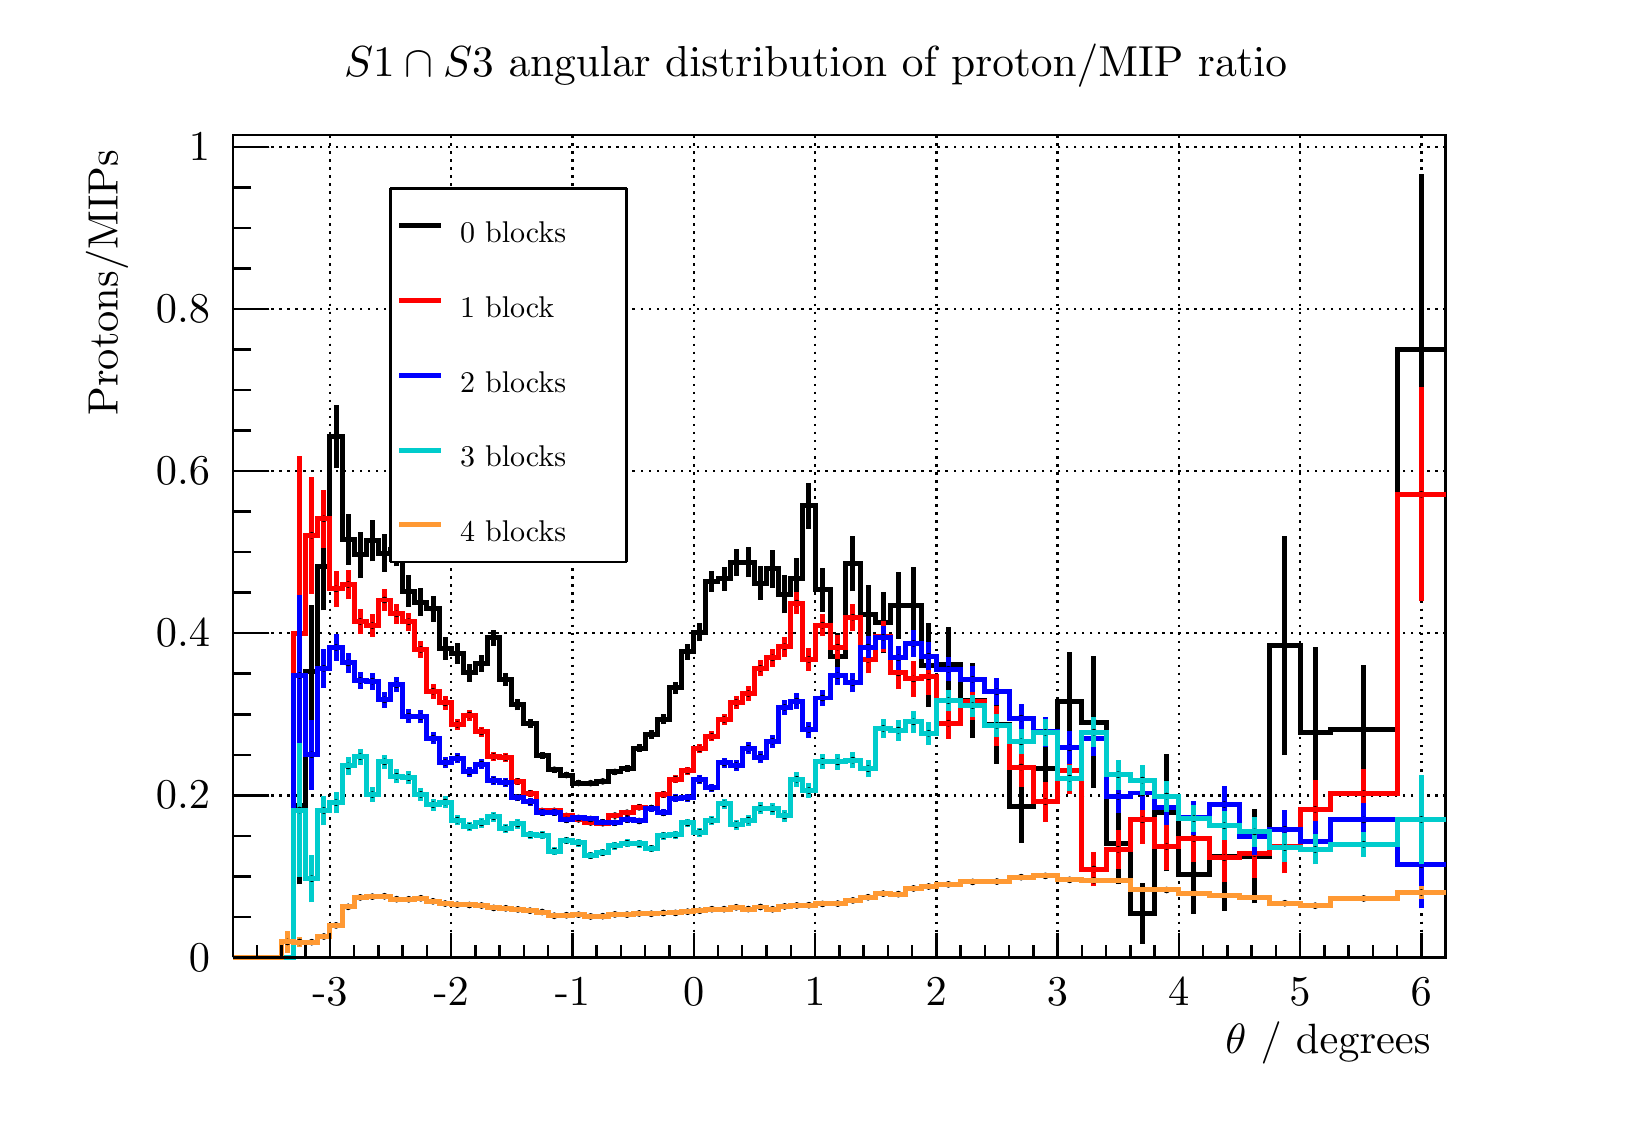
\begin{tikzpicture}
\pgfdeclareplotmark{cross} {
\pgfpathmoveto{\pgfpoint{-0.3\pgfplotmarksize}{\pgfplotmarksize}}
\pgfpathlineto{\pgfpoint{+0.3\pgfplotmarksize}{\pgfplotmarksize}}
\pgfpathlineto{\pgfpoint{+0.3\pgfplotmarksize}{0.3\pgfplotmarksize}}
\pgfpathlineto{\pgfpoint{+1\pgfplotmarksize}{0.3\pgfplotmarksize}}
\pgfpathlineto{\pgfpoint{+1\pgfplotmarksize}{-0.3\pgfplotmarksize}}
\pgfpathlineto{\pgfpoint{+0.3\pgfplotmarksize}{-0.3\pgfplotmarksize}}
\pgfpathlineto{\pgfpoint{+0.3\pgfplotmarksize}{-1.\pgfplotmarksize}}
\pgfpathlineto{\pgfpoint{-0.3\pgfplotmarksize}{-1.\pgfplotmarksize}}
\pgfpathlineto{\pgfpoint{-0.3\pgfplotmarksize}{-0.3\pgfplotmarksize}}
\pgfpathlineto{\pgfpoint{-1.\pgfplotmarksize}{-0.3\pgfplotmarksize}}
\pgfpathlineto{\pgfpoint{-1.\pgfplotmarksize}{0.3\pgfplotmarksize}}
\pgfpathlineto{\pgfpoint{-0.3\pgfplotmarksize}{0.3\pgfplotmarksize}}
\pgfpathclose
\pgfusepathqstroke
}
\pgfdeclareplotmark{cross*} {
\pgfpathmoveto{\pgfpoint{-0.3\pgfplotmarksize}{\pgfplotmarksize}}
\pgfpathlineto{\pgfpoint{+0.3\pgfplotmarksize}{\pgfplotmarksize}}
\pgfpathlineto{\pgfpoint{+0.3\pgfplotmarksize}{0.3\pgfplotmarksize}}
\pgfpathlineto{\pgfpoint{+1\pgfplotmarksize}{0.3\pgfplotmarksize}}
\pgfpathlineto{\pgfpoint{+1\pgfplotmarksize}{-0.3\pgfplotmarksize}}
\pgfpathlineto{\pgfpoint{+0.3\pgfplotmarksize}{-0.3\pgfplotmarksize}}
\pgfpathlineto{\pgfpoint{+0.3\pgfplotmarksize}{-1.\pgfplotmarksize}}
\pgfpathlineto{\pgfpoint{-0.3\pgfplotmarksize}{-1.\pgfplotmarksize}}
\pgfpathlineto{\pgfpoint{-0.3\pgfplotmarksize}{-0.3\pgfplotmarksize}}
\pgfpathlineto{\pgfpoint{-1.\pgfplotmarksize}{-0.3\pgfplotmarksize}}
\pgfpathlineto{\pgfpoint{-1.\pgfplotmarksize}{0.3\pgfplotmarksize}}
\pgfpathlineto{\pgfpoint{-0.3\pgfplotmarksize}{0.3\pgfplotmarksize}}
\pgfpathclose
\pgfusepathqfillstroke
}
\pgfdeclareplotmark{newstar} {
\pgfpathmoveto{\pgfqpoint{0pt}{\pgfplotmarksize}}
\pgfpathlineto{\pgfqpointpolar{44}{0.5\pgfplotmarksize}}
\pgfpathlineto{\pgfqpointpolar{18}{\pgfplotmarksize}}
\pgfpathlineto{\pgfqpointpolar{-20}{0.5\pgfplotmarksize}}
\pgfpathlineto{\pgfqpointpolar{-54}{\pgfplotmarksize}}
\pgfpathlineto{\pgfqpointpolar{-90}{0.5\pgfplotmarksize}}
\pgfpathlineto{\pgfqpointpolar{234}{\pgfplotmarksize}}
\pgfpathlineto{\pgfqpointpolar{198}{0.5\pgfplotmarksize}}
\pgfpathlineto{\pgfqpointpolar{162}{\pgfplotmarksize}}
\pgfpathlineto{\pgfqpointpolar{134}{0.5\pgfplotmarksize}}
\pgfpathclose
\pgfusepathqstroke
}
\pgfdeclareplotmark{newstar*} {
\pgfpathmoveto{\pgfqpoint{0pt}{\pgfplotmarksize}}
\pgfpathlineto{\pgfqpointpolar{44}{0.5\pgfplotmarksize}}
\pgfpathlineto{\pgfqpointpolar{18}{\pgfplotmarksize}}
\pgfpathlineto{\pgfqpointpolar{-20}{0.5\pgfplotmarksize}}
\pgfpathlineto{\pgfqpointpolar{-54}{\pgfplotmarksize}}
\pgfpathlineto{\pgfqpointpolar{-90}{0.5\pgfplotmarksize}}
\pgfpathlineto{\pgfqpointpolar{234}{\pgfplotmarksize}}
\pgfpathlineto{\pgfqpointpolar{198}{0.5\pgfplotmarksize}}
\pgfpathlineto{\pgfqpointpolar{162}{\pgfplotmarksize}}
\pgfpathlineto{\pgfqpointpolar{134}{0.5\pgfplotmarksize}}
\pgfpathclose
\pgfusepathqfillstroke
}
\definecolor{c}{rgb}{1,1,1};
\draw [color=c, fill=c] (0,0) rectangle (20,13.5632);
\draw [color=c, fill=c] (2.6,1.76322) rectangle (18,12.2069);
\definecolor{c}{rgb}{0,0,0};
\draw [c,line width=0.9] (2.6,1.76322) -- (2.6,12.2069) -- (18,12.2069) -- (18,1.76322) -- (2.6,1.76322);
\definecolor{c}{rgb}{1,1,1};
\draw [color=c, fill=c] (2.6,1.76322) rectangle (18,12.2069);
\definecolor{c}{rgb}{0,0,0};
\draw [c,line width=0.9] (2.6,1.76322) -- (2.6,12.2069) -- (18,12.2069) -- (18,1.76322) -- (2.6,1.76322);
\draw [c,line width=0.9] (2.6,1.76322) -- (18,1.76322);
\draw [c,dotted,line width=0.9] (3.832,12.2069) -- (3.832,1.76322);
\draw [c,dotted,line width=0.9] (5.372,12.2069) -- (5.372,1.76322);
\draw [c,dotted,line width=0.9] (6.912,12.2069) -- (6.912,1.76322);
\draw [c,dotted,line width=0.9] (8.452,12.2069) -- (8.452,1.76322);
\draw [c,dotted,line width=0.9] (9.992,12.2069) -- (9.992,1.76322);
\draw [c,dotted,line width=0.9] (11.532,12.2069) -- (11.532,1.76322);
\draw [c,dotted,line width=0.9] (13.072,12.2069) -- (13.072,1.76322);
\draw [c,dotted,line width=0.9] (14.612,12.2069) -- (14.612,1.76322);
\draw [c,dotted,line width=0.9] (16.152,12.2069) -- (16.152,1.76322);
\draw [c,dotted,line width=0.9] (17.692,12.2069) -- (17.692,1.76322);
\draw [c,dotted,line width=0.9] (3.832,12.2069) -- (3.832,1.76322);
\draw [c,dotted,line width=0.9] (17.692,12.2069) -- (17.692,1.76322);
\draw [c,line width=0.9] (2.6,1.76322) -- (2.6,12.2069);
\draw [c,dotted,line width=0.9] (18,1.76322) -- (2.6,1.76322);
\draw [c,dotted,line width=0.9] (18,3.82143) -- (2.6,3.82143);
\draw [c,dotted,line width=0.9] (18,5.87964) -- (2.6,5.87964);
\draw [c,dotted,line width=0.9] (18,7.93785) -- (2.6,7.93785);
\draw [c,dotted,line width=0.9] (18,9.99605) -- (2.6,9.99605);
\draw [c,dotted,line width=0.9] (18,12.0543) -- (2.6,12.0543);
\draw [c,dotted,line width=0.9] (18,12.0543) -- (2.6,12.0543);
\definecolor{c}{rgb}{0,0,0.6};
\draw [c,line width=0.9] (2.6,1.76322) -- (2.754,1.76322) -- (2.754,1.76322) -- (2.908,1.76322) -- (2.908,1.76322) -- (3.062,1.76322) -- (3.062,1.76322) -- (3.216,1.76322) -- (3.216,1.76322) -- (3.37,1.76322) -- (3.37,1.76322) -- (3.524,1.76322) --
 (3.524,1.76322) -- (3.678,1.76322) -- (3.678,1.76322) -- (3.832,1.76322) -- (3.832,1.76322) -- (3.986,1.76322) -- (3.986,1.76322) -- (4.14,1.76322) -- (4.14,1.76322) -- (4.294,1.76322) -- (4.294,1.76322) -- (4.448,1.76322) -- (4.448,1.76322) --
 (4.602,1.76322) -- (4.602,1.76322) -- (4.756,1.76322) -- (4.756,1.76322) -- (4.91,1.76322) -- (4.91,1.76322) -- (5.064,1.76322) -- (5.064,1.76322) -- (5.218,1.76322) -- (5.218,1.76322) -- (5.372,1.76322) -- (5.372,1.76322) -- (5.526,1.76322) --
 (5.526,1.76322) -- (5.68,1.76322) -- (5.68,1.76322) -- (5.834,1.76322) -- (5.834,1.76322) -- (5.988,1.76322) -- (5.988,1.76322) -- (6.142,1.76322) -- (6.142,1.76322) -- (6.296,1.76322) -- (6.296,1.76322) -- (6.45,1.76322) -- (6.45,1.76322) --
 (6.604,1.76322) -- (6.604,1.76322) -- (6.758,1.76322) -- (6.758,1.76322) -- (6.912,1.76322) -- (6.912,1.76322) -- (7.066,1.76322) -- (7.066,1.76322) -- (7.22,1.76322) -- (7.22,1.76322) -- (7.374,1.76322) -- (7.374,1.76322) -- (7.528,1.76322) --
 (7.528,1.76322) -- (7.682,1.76322) -- (7.682,1.76322) -- (7.836,1.76322) -- (7.836,1.76322) -- (7.99,1.76322) -- (7.99,1.76322) -- (8.144,1.76322) -- (8.144,1.76322) -- (8.298,1.76322) -- (8.298,1.76322) -- (8.452,1.76322) -- (8.452,1.76322) --
 (8.606,1.76322) -- (8.606,1.76322) -- (8.76,1.76322) -- (8.76,1.76322) -- (8.914,1.76322) -- (8.914,1.76322) -- (9.068,1.76322) -- (9.068,1.76322) -- (9.222,1.76322) -- (9.222,1.76322) -- (9.376,1.76322) -- (9.376,1.76322) -- (9.53,1.76322) --
 (9.53,1.76322) -- (9.684,1.76322) -- (9.684,1.76322) -- (9.838,1.76322) -- (9.838,1.76322) -- (9.992,1.76322) -- (9.992,1.76322) -- (10.1845,1.76322) -- (10.1845,1.76322) -- (10.377,1.76322) -- (10.377,1.76322) -- (10.5695,1.76322) --
 (10.5695,1.76322) -- (10.762,1.76322) -- (10.762,1.76322) -- (10.9545,1.76322) -- (10.9545,1.76322) -- (11.147,1.76322) -- (11.147,1.76322) -- (11.3395,1.76322) -- (11.3395,1.76322) -- (11.532,1.76322) -- (11.532,1.76322) -- (11.84,1.76322) --
 (11.84,1.76322) -- (12.148,1.76322) -- (12.148,1.76322) -- (12.456,1.76322) -- (12.456,1.76322) -- (12.764,1.76322) -- (12.764,1.76322) -- (13.072,1.76322) -- (13.072,1.76322) -- (13.38,1.76322) -- (13.38,1.76322) -- (13.688,1.76322) --
 (13.688,1.76322) -- (13.996,1.76322) -- (13.996,1.76322) -- (14.304,1.76322) -- (14.304,1.76322) -- (14.612,1.76322) -- (14.612,1.76322) -- (14.997,1.76322) -- (14.997,1.76322) -- (15.382,1.76322) -- (15.382,1.76322) -- (15.767,1.76322) --
 (15.767,1.76322) -- (16.152,1.76322) -- (16.152,1.76322) -- (16.537,1.76322) -- (16.537,1.76322) -- (17.384,1.76322) -- (17.384,1.76322) -- (18,1.76322);
\definecolor{c}{rgb}{0,0,0};
\draw [c,line width=0.9] (2.6,1.76322) -- (18,1.76322);
\draw [anchor= east] (18,0.678161) node[scale=1.5317, color=c, rotate=0]{$\theta$ / degrees};
\draw [c,line width=0.9] (3.832,2.07653) -- (3.832,1.76322);
\draw [c,line width=0.9] (4.14,1.91987) -- (4.14,1.76322);
\draw [c,line width=0.9] (4.448,1.91987) -- (4.448,1.76322);
\draw [c,line width=0.9] (4.756,1.91987) -- (4.756,1.76322);
\draw [c,line width=0.9] (5.064,1.91987) -- (5.064,1.76322);
\draw [c,line width=0.9] (5.372,2.07653) -- (5.372,1.76322);
\draw [c,line width=0.9] (5.68,1.91987) -- (5.68,1.76322);
\draw [c,line width=0.9] (5.988,1.91987) -- (5.988,1.76322);
\draw [c,line width=0.9] (6.296,1.91987) -- (6.296,1.76322);
\draw [c,line width=0.9] (6.604,1.91987) -- (6.604,1.76322);
\draw [c,line width=0.9] (6.912,2.07653) -- (6.912,1.76322);
\draw [c,line width=0.9] (7.22,1.91987) -- (7.22,1.76322);
\draw [c,line width=0.9] (7.528,1.91987) -- (7.528,1.76322);
\draw [c,line width=0.9] (7.836,1.91987) -- (7.836,1.76322);
\draw [c,line width=0.9] (8.144,1.91987) -- (8.144,1.76322);
\draw [c,line width=0.9] (8.452,2.07653) -- (8.452,1.76322);
\draw [c,line width=0.9] (8.76,1.91987) -- (8.76,1.76322);
\draw [c,line width=0.9] (9.068,1.91987) -- (9.068,1.76322);
\draw [c,line width=0.9] (9.376,1.91987) -- (9.376,1.76322);
\draw [c,line width=0.9] (9.684,1.91987) -- (9.684,1.76322);
\draw [c,line width=0.9] (9.992,2.07653) -- (9.992,1.76322);
\draw [c,line width=0.9] (10.3,1.91987) -- (10.3,1.76322);
\draw [c,line width=0.9] (10.608,1.91987) -- (10.608,1.76322);
\draw [c,line width=0.9] (10.916,1.91987) -- (10.916,1.76322);
\draw [c,line width=0.9] (11.224,1.91987) -- (11.224,1.76322);
\draw [c,line width=0.9] (11.532,2.07653) -- (11.532,1.76322);
\draw [c,line width=0.9] (11.84,1.91987) -- (11.84,1.76322);
\draw [c,line width=0.9] (12.148,1.91987) -- (12.148,1.76322);
\draw [c,line width=0.9] (12.456,1.91987) -- (12.456,1.76322);
\draw [c,line width=0.9] (12.764,1.91987) -- (12.764,1.76322);
\draw [c,line width=0.9] (13.072,2.07653) -- (13.072,1.76322);
\draw [c,line width=0.9] (13.38,1.91987) -- (13.38,1.76322);
\draw [c,line width=0.9] (13.688,1.91987) -- (13.688,1.76322);
\draw [c,line width=0.9] (13.996,1.91987) -- (13.996,1.76322);
\draw [c,line width=0.9] (14.304,1.91987) -- (14.304,1.76322);
\draw [c,line width=0.9] (14.612,2.07653) -- (14.612,1.76322);
\draw [c,line width=0.9] (14.92,1.91987) -- (14.92,1.76322);
\draw [c,line width=0.9] (15.228,1.91987) -- (15.228,1.76322);
\draw [c,line width=0.9] (15.536,1.91987) -- (15.536,1.76322);
\draw [c,line width=0.9] (15.844,1.91987) -- (15.844,1.76322);
\draw [c,line width=0.9] (16.152,2.07653) -- (16.152,1.76322);
\draw [c,line width=0.9] (16.46,1.91987) -- (16.46,1.76322);
\draw [c,line width=0.9] (16.768,1.91987) -- (16.768,1.76322);
\draw [c,line width=0.9] (17.076,1.91987) -- (17.076,1.76322);
\draw [c,line width=0.9] (17.384,1.91987) -- (17.384,1.76322);
\draw [c,line width=0.9] (17.692,2.07653) -- (17.692,1.76322);
\draw [c,line width=0.9] (3.832,2.07653) -- (3.832,1.76322);
\draw [c,line width=0.9] (3.524,1.91987) -- (3.524,1.76322);
\draw [c,line width=0.9] (3.216,1.91987) -- (3.216,1.76322);
\draw [c,line width=0.9] (2.908,1.91987) -- (2.908,1.76322);
\draw [c,line width=0.9] (17.692,2.07653) -- (17.692,1.76322);
\draw [anchor=base] (3.832,1.15287) node[scale=1.5317, color=c, rotate=0]{-3};
\draw [anchor=base] (5.372,1.15287) node[scale=1.5317, color=c, rotate=0]{-2};
\draw [anchor=base] (6.912,1.15287) node[scale=1.5317, color=c, rotate=0]{-1};
\draw [anchor=base] (8.452,1.15287) node[scale=1.5317, color=c, rotate=0]{0};
\draw [anchor=base] (9.992,1.15287) node[scale=1.5317, color=c, rotate=0]{1};
\draw [anchor=base] (11.532,1.15287) node[scale=1.5317, color=c, rotate=0]{2};
\draw [anchor=base] (13.072,1.15287) node[scale=1.5317, color=c, rotate=0]{3};
\draw [anchor=base] (14.612,1.15287) node[scale=1.5317, color=c, rotate=0]{4};
\draw [anchor=base] (16.152,1.15287) node[scale=1.5317, color=c, rotate=0]{5};
\draw [anchor=base] (17.692,1.15287) node[scale=1.5317, color=c, rotate=0]{6};
\draw [c,line width=0.9] (2.6,1.76322) -- (2.6,12.2069);
\draw [anchor= east] (1,12.2069) node[scale=1.5317, color=c, rotate=90]{  Protons/MIPs};
\draw [c,line width=0.9] (3.062,1.76322) -- (2.6,1.76322);
\draw [c,line width=0.9] (2.831,2.27777) -- (2.6,2.27777);
\draw [c,line width=0.9] (2.831,2.79232) -- (2.6,2.79232);
\draw [c,line width=0.9] (2.831,3.30687) -- (2.6,3.30687);
\draw [c,line width=0.9] (3.062,3.82143) -- (2.6,3.82143);
\draw [c,line width=0.9] (2.831,4.33598) -- (2.6,4.33598);
\draw [c,line width=0.9] (2.831,4.85053) -- (2.6,4.85053);
\draw [c,line width=0.9] (2.831,5.36508) -- (2.6,5.36508);
\draw [c,line width=0.9] (3.062,5.87964) -- (2.6,5.87964);
\draw [c,line width=0.9] (2.831,6.39419) -- (2.6,6.39419);
\draw [c,line width=0.9] (2.831,6.90874) -- (2.6,6.90874);
\draw [c,line width=0.9] (2.831,7.42329) -- (2.6,7.42329);
\draw [c,line width=0.9] (3.062,7.93785) -- (2.6,7.93785);
\draw [c,line width=0.9] (2.831,8.4524) -- (2.6,8.4524);
\draw [c,line width=0.9] (2.831,8.96695) -- (2.6,8.96695);
\draw [c,line width=0.9] (2.831,9.4815) -- (2.6,9.4815);
\draw [c,line width=0.9] (3.062,9.99605) -- (2.6,9.99605);
\draw [c,line width=0.9] (2.831,10.5106) -- (2.6,10.5106);
\draw [c,line width=0.9] (2.831,11.0252) -- (2.6,11.0252);
\draw [c,line width=0.9] (2.831,11.5397) -- (2.6,11.5397);
\draw [c,line width=0.9] (3.062,12.0543) -- (2.6,12.0543);
\draw [c,line width=0.9] (3.062,12.0543) -- (2.6,12.0543);
\draw [anchor= east] (2.5,1.76322) node[scale=1.5317, color=c, rotate=0]{0};
\draw [anchor= east] (2.5,3.82143) node[scale=1.5317, color=c, rotate=0]{0.2};
\draw [anchor= east] (2.5,5.87964) node[scale=1.5317, color=c, rotate=0]{0.4};
\draw [anchor= east] (2.5,7.93785) node[scale=1.5317, color=c, rotate=0]{0.6};
\draw [anchor= east] (2.5,9.99605) node[scale=1.5317, color=c, rotate=0]{0.8};
\draw [anchor= east] (2.5,12.0543) node[scale=1.5317, color=c, rotate=0]{1};
\draw [c,line width=1.8] (3.447,2.68861) -- (3.447,3.69279);
\draw [c,line width=1.8] (3.447,3.69279) -- (3.447,4.69697);
\foreach \P in {(3.447,3.69279)}{\draw[mark options={color=c,fill=c},mark size=2.402402pt,mark=*,mark size=1pt] plot coordinates {\P};}
\draw [c,line width=1.8] (3.601,4.55193) -- (3.601,5.39535);
\draw [c,line width=1.8] (3.601,5.39535) -- (3.601,6.23877);
\foreach \P in {(3.601,5.39535)}{\draw[mark options={color=c,fill=c},mark size=2.402402pt,mark=*,mark size=1pt] plot coordinates {\P};}
\draw [c,line width=1.8] (3.755,6.16937) -- (3.755,6.72713);
\draw [c,line width=1.8] (3.755,6.72713) -- (3.755,7.2849);
\foreach \P in {(3.755,6.72713)}{\draw[mark options={color=c,fill=c},mark size=2.402402pt,mark=*,mark size=1pt] plot coordinates {\P};}
\draw [c,line width=1.8] (3.909,7.97262) -- (3.909,8.37402);
\draw [c,line width=1.8] (3.909,8.37402) -- (3.909,8.77542);
\foreach \P in {(3.909,8.37402)}{\draw[mark options={color=c,fill=c},mark size=2.402402pt,mark=*,mark size=1pt] plot coordinates {\P};}
\draw [c,line width=1.8] (4.063,6.74812) -- (4.063,7.07209);
\draw [c,line width=1.8] (4.063,7.07209) -- (4.063,7.39606);
\foreach \P in {(4.063,7.07209)}{\draw[mark options={color=c,fill=c},mark size=2.402402pt,mark=*,mark size=1pt] plot coordinates {\P};}
\draw [c,line width=1.8] (4.217,6.57737) -- (4.217,6.87444);
\draw [c,line width=1.8] (4.217,6.87444) -- (4.217,7.17151);
\foreach \P in {(4.217,6.87444)}{\draw[mark options={color=c,fill=c},mark size=2.402402pt,mark=*,mark size=1pt] plot coordinates {\P};}
\draw [c,line width=1.8] (4.371,6.79338) -- (4.371,7.0535);
\draw [c,line width=1.8] (4.371,7.0535) -- (4.371,7.31362);
\foreach \P in {(4.371,7.0535)}{\draw[mark options={color=c,fill=c},mark size=2.402402pt,mark=*,mark size=1pt] plot coordinates {\P};}
\draw [c,line width=1.8] (4.525,6.65736) -- (4.525,6.89753);
\draw [c,line width=1.8] (4.525,6.89753) -- (4.525,7.1377);
\foreach \P in {(4.525,6.89753)}{\draw[mark options={color=c,fill=c},mark size=2.402402pt,mark=*,mark size=1pt] plot coordinates {\P};}
\draw [c,line width=1.8] (4.679,6.72958) -- (4.679,6.94472);
\draw [c,line width=1.8] (4.679,6.94472) -- (4.679,7.15986);
\foreach \P in {(4.679,6.94472)}{\draw[mark options={color=c,fill=c},mark size=2.402402pt,mark=*,mark size=1pt] plot coordinates {\P};}
\draw [c,line width=1.8] (4.833,6.21551) -- (4.833,6.41533);
\draw [c,line width=1.8] (4.833,6.41533) -- (4.833,6.61516);
\foreach \P in {(4.833,6.41533)}{\draw[mark options={color=c,fill=c},mark size=2.402402pt,mark=*,mark size=1pt] plot coordinates {\P};}
\draw [c,line width=1.8] (4.987,6.09559) -- (4.987,6.2725);
\draw [c,line width=1.8] (4.987,6.2725) -- (4.987,6.44941);
\foreach \P in {(4.987,6.2725)}{\draw[mark options={color=c,fill=c},mark size=2.402402pt,mark=*,mark size=1pt] plot coordinates {\P};}
\draw [c,line width=1.8] (5.141,6.02679) -- (5.141,6.18847);
\draw [c,line width=1.8] (5.141,6.18847) -- (5.141,6.35015);
\foreach \P in {(5.141,6.18847)}{\draw[mark options={color=c,fill=c},mark size=2.402402pt,mark=*,mark size=1pt] plot coordinates {\P};}
\draw [c,line width=1.8] (5.295,5.54014) -- (5.295,5.68527);
\draw [c,line width=1.8] (5.295,5.68527) -- (5.295,5.8304);
\foreach \P in {(5.295,5.68527)}{\draw[mark options={color=c,fill=c},mark size=2.402402pt,mark=*,mark size=1pt] plot coordinates {\P};}
\draw [c,line width=1.8] (5.449,5.49417) -- (5.449,5.62692);
\draw [c,line width=1.8] (5.449,5.62692) -- (5.449,5.75968);
\foreach \P in {(5.449,5.62692)}{\draw[mark options={color=c,fill=c},mark size=2.402402pt,mark=*,mark size=1pt] plot coordinates {\P};}
\draw [c,line width=1.8] (5.603,5.26127) -- (5.603,5.3782);
\draw [c,line width=1.8] (5.603,5.3782) -- (5.603,5.49514);
\foreach \P in {(5.603,5.3782)}{\draw[mark options={color=c,fill=c},mark size=2.402402pt,mark=*,mark size=1pt] plot coordinates {\P};}
\draw [c,line width=1.8] (5.757,5.38457) -- (5.757,5.4911);
\draw [c,line width=1.8] (5.757,5.4911) -- (5.757,5.59762);
\foreach \P in {(5.757,5.4911)}{\draw[mark options={color=c,fill=c},mark size=2.402402pt,mark=*,mark size=1pt] plot coordinates {\P};}
\draw [c,line width=1.8] (5.911,5.72283) -- (5.911,5.82056);
\draw [c,line width=1.8] (5.911,5.82056) -- (5.911,5.9183);
\foreach \P in {(5.911,5.82056)}{\draw[mark options={color=c,fill=c},mark size=2.402402pt,mark=*,mark size=1pt] plot coordinates {\P};}
\draw [c,line width=1.8] (6.065,5.20876) -- (6.065,5.29262);
\draw [c,line width=1.8] (6.065,5.29262) -- (6.065,5.37647);
\foreach \P in {(6.065,5.29262)}{\draw[mark options={color=c,fill=c},mark size=2.402402pt,mark=*,mark size=1pt] plot coordinates {\P};}
\draw [c,line width=1.8] (6.219,4.90059) -- (6.219,4.97013);
\draw [c,line width=1.8] (6.219,4.97013) -- (6.219,5.03967);
\foreach \P in {(6.219,4.97013)}{\draw[mark options={color=c,fill=c},mark size=2.402402pt,mark=*,mark size=1pt] plot coordinates {\P};}
\draw [c,line width=1.8] (6.373,4.67441) -- (6.373,4.73269);
\draw [c,line width=1.8] (6.373,4.73269) -- (6.373,4.79097);
\foreach \P in {(6.373,4.73269)}{\draw[mark options={color=c,fill=c},mark size=2.402402pt,mark=*,mark size=1pt] plot coordinates {\P};}
\draw [c,line width=1.8] (6.527,4.27936) -- (6.527,4.32689);
\draw [c,line width=1.8] (6.527,4.32689) -- (6.527,4.37441);
\foreach \P in {(6.527,4.32689)}{\draw[mark options={color=c,fill=c},mark size=2.402402pt,mark=*,mark size=1pt] plot coordinates {\P};}
\draw [c,line width=1.8] (6.681,4.10644) -- (6.681,4.14662);
\draw [c,line width=1.8] (6.681,4.14662) -- (6.681,4.18681);
\foreach \P in {(6.681,4.14662)}{\draw[mark options={color=c,fill=c},mark size=2.402402pt,mark=*,mark size=1pt] plot coordinates {\P};}
\draw [c,line width=1.8] (6.835,4.04256) -- (6.835,4.07876);
\draw [c,line width=1.8] (6.835,4.07876) -- (6.835,4.11496);
\foreach \P in {(6.835,4.07876)}{\draw[mark options={color=c,fill=c},mark size=2.402402pt,mark=*,mark size=1pt] plot coordinates {\P};}
\draw [c,line width=1.8] (6.989,3.94346) -- (6.989,3.97699);
\draw [c,line width=1.8] (6.989,3.97699) -- (6.989,4.01053);
\foreach \P in {(6.989,3.97699)}{\draw[mark options={color=c,fill=c},mark size=2.402402pt,mark=*,mark size=1pt] plot coordinates {\P};}
\draw [c,line width=1.8] (7.143,3.94258) -- (7.143,3.97579);
\draw [c,line width=1.8] (7.143,3.97579) -- (7.143,4.00901);
\foreach \P in {(7.143,3.97579)}{\draw[mark options={color=c,fill=c},mark size=2.402402pt,mark=*,mark size=1pt] plot coordinates {\P};}
\draw [c,line width=1.8] (7.297,3.96395) -- (7.297,3.99829);
\draw [c,line width=1.8] (7.297,3.99829) -- (7.297,4.03263);
\foreach \P in {(7.297,3.99829)}{\draw[mark options={color=c,fill=c},mark size=2.402402pt,mark=*,mark size=1pt] plot coordinates {\P};}
\draw [c,line width=1.8] (7.451,4.08086) -- (7.451,4.11859);
\draw [c,line width=1.8] (7.451,4.11859) -- (7.451,4.15633);
\foreach \P in {(7.451,4.11859)}{\draw[mark options={color=c,fill=c},mark size=2.402402pt,mark=*,mark size=1pt] plot coordinates {\P};}
\draw [c,line width=1.8] (7.605,4.11965) -- (7.605,4.1614);
\draw [c,line width=1.8] (7.605,4.1614) -- (7.605,4.20315);
\foreach \P in {(7.605,4.1614)}{\draw[mark options={color=c,fill=c},mark size=2.402402pt,mark=*,mark size=1pt] plot coordinates {\P};}
\draw [c,line width=1.8] (7.759,4.37305) -- (7.759,4.42142);
\draw [c,line width=1.8] (7.759,4.42142) -- (7.759,4.46979);
\foreach \P in {(7.759,4.42142)}{\draw[mark options={color=c,fill=c},mark size=2.402402pt,mark=*,mark size=1pt] plot coordinates {\P};}
\draw [c,line width=1.8] (7.913,4.53427) -- (7.913,4.5899);
\draw [c,line width=1.8] (7.913,4.5899) -- (7.913,4.64552);
\foreach \P in {(7.913,4.5899)}{\draw[mark options={color=c,fill=c},mark size=2.402402pt,mark=*,mark size=1pt] plot coordinates {\P};}
\draw [c,line width=1.8] (8.067,4.72215) -- (8.067,4.78731);
\draw [c,line width=1.8] (8.067,4.78731) -- (8.067,4.85247);
\foreach \P in {(8.067,4.78731)}{\draw[mark options={color=c,fill=c},mark size=2.402402pt,mark=*,mark size=1pt] plot coordinates {\P};}
\draw [c,line width=1.8] (8.221,5.10467) -- (8.221,5.18431);
\draw [c,line width=1.8] (8.221,5.18431) -- (8.221,5.26395);
\foreach \P in {(8.221,5.18431)}{\draw[mark options={color=c,fill=c},mark size=2.402402pt,mark=*,mark size=1pt] plot coordinates {\P};}
\draw [c,line width=1.8] (8.375,5.5447) -- (8.375,5.64191);
\draw [c,line width=1.8] (8.375,5.64191) -- (8.375,5.73912);
\foreach \P in {(8.375,5.64191)}{\draw[mark options={color=c,fill=c},mark size=2.402402pt,mark=*,mark size=1pt] plot coordinates {\P};}
\draw [c,line width=1.8] (8.529,5.77689) -- (8.529,5.89264);
\draw [c,line width=1.8] (8.529,5.89264) -- (8.529,6.00839);
\foreach \P in {(8.529,5.89264)}{\draw[mark options={color=c,fill=c},mark size=2.402402pt,mark=*,mark size=1pt] plot coordinates {\P};}
\draw [c,line width=1.8] (8.683,6.40553) -- (8.683,6.53755);
\draw [c,line width=1.8] (8.683,6.53755) -- (8.683,6.66958);
\foreach \P in {(8.683,6.53755)}{\draw[mark options={color=c,fill=c},mark size=2.402402pt,mark=*,mark size=1pt] plot coordinates {\P};}
\draw [c,line width=1.8] (8.837,6.41976) -- (8.837,6.57237);
\draw [c,line width=1.8] (8.837,6.57237) -- (8.837,6.72498);
\foreach \P in {(8.837,6.57237)}{\draw[mark options={color=c,fill=c},mark size=2.402402pt,mark=*,mark size=1pt] plot coordinates {\P};}
\draw [c,line width=1.8] (8.991,6.6065) -- (8.991,6.77768);
\draw [c,line width=1.8] (8.991,6.77768) -- (8.991,6.94886);
\foreach \P in {(8.991,6.77768)}{\draw[mark options={color=c,fill=c},mark size=2.402402pt,mark=*,mark size=1pt] plot coordinates {\P};}
\draw [c,line width=1.8] (9.145,6.59087) -- (9.145,6.78152);
\draw [c,line width=1.8] (9.145,6.78152) -- (9.145,6.97216);
\foreach \P in {(9.145,6.78152)}{\draw[mark options={color=c,fill=c},mark size=2.402402pt,mark=*,mark size=1pt] plot coordinates {\P};}
\draw [c,line width=1.8] (9.299,6.30591) -- (9.299,6.51695);
\draw [c,line width=1.8] (9.299,6.51695) -- (9.299,6.72799);
\foreach \P in {(9.299,6.51695)}{\draw[mark options={color=c,fill=c},mark size=2.402402pt,mark=*,mark size=1pt] plot coordinates {\P};}
\draw [c,line width=1.8] (9.453,6.45578) -- (9.453,6.69574);
\draw [c,line width=1.8] (9.453,6.69574) -- (9.453,6.93571);
\foreach \P in {(9.453,6.69574)}{\draw[mark options={color=c,fill=c},mark size=2.402402pt,mark=*,mark size=1pt] plot coordinates {\P};}
\draw [c,line width=1.8] (9.607,6.13276) -- (9.607,6.37565);
\draw [c,line width=1.8] (9.607,6.37565) -- (9.607,6.61853);
\foreach \P in {(9.607,6.37565)}{\draw[mark options={color=c,fill=c},mark size=2.402402pt,mark=*,mark size=1pt] plot coordinates {\P};}
\draw [c,line width=1.8] (9.761,6.30551) -- (9.761,6.57316);
\draw [c,line width=1.8] (9.761,6.57316) -- (9.761,6.84082);
\foreach \P in {(9.761,6.57316)}{\draw[mark options={color=c,fill=c},mark size=2.402402pt,mark=*,mark size=1pt] plot coordinates {\P};}
\draw [c,line width=1.8] (9.915,7.20652) -- (9.915,7.49921);
\draw [c,line width=1.8] (9.915,7.49921) -- (9.915,7.7919);
\foreach \P in {(9.915,7.49921)}{\draw[mark options={color=c,fill=c},mark size=2.402402pt,mark=*,mark size=1pt] plot coordinates {\P};}
\draw [c,line width=1.8] (10.0883,6.15266) -- (10.0883,6.43259);
\draw [c,line width=1.8] (10.0883,6.43259) -- (10.0883,6.71251);
\foreach \P in {(10.0883,6.43259)}{\draw[mark options={color=c,fill=c},mark size=2.402402pt,mark=*,mark size=1pt] plot coordinates {\P};}
\draw [c,line width=1.8] (10.2808,5.28593) -- (10.2808,5.58145);
\draw [c,line width=1.8] (10.2808,5.58145) -- (10.2808,5.87697);
\foreach \P in {(10.2808,5.58145)}{\draw[mark options={color=c,fill=c},mark size=2.402402pt,mark=*,mark size=1pt] plot coordinates {\P};}
\draw [c,line width=1.8] (10.4733,6.40986) -- (10.4733,6.76311);
\draw [c,line width=1.8] (10.4733,6.76311) -- (10.4733,7.11637);
\foreach \P in {(10.4733,6.76311)}{\draw[mark options={color=c,fill=c},mark size=2.402402pt,mark=*,mark size=1pt] plot coordinates {\P};}
\draw [c,line width=1.8] (10.6657,5.74025) -- (10.6657,6.11712);
\draw [c,line width=1.8] (10.6657,6.11712) -- (10.6657,6.49399);
\foreach \P in {(10.6657,6.11712)}{\draw[mark options={color=c,fill=c},mark size=2.402402pt,mark=*,mark size=1pt] plot coordinates {\P};}
\draw [c,line width=1.8] (10.8582,5.62308) -- (10.8582,6.01521);
\draw [c,line width=1.8] (10.8582,6.01521) -- (10.8582,6.40733);
\foreach \P in {(10.8582,6.01521)}{\draw[mark options={color=c,fill=c},mark size=2.402402pt,mark=*,mark size=1pt] plot coordinates {\P};}
\draw [c,line width=1.8] (11.0507,5.81087) -- (11.0507,6.2345);
\draw [c,line width=1.8] (11.0507,6.2345) -- (11.0507,6.65813);
\foreach \P in {(11.0507,6.2345)}{\draw[mark options={color=c,fill=c},mark size=2.402402pt,mark=*,mark size=1pt] plot coordinates {\P};}
\draw [c,line width=1.8] (11.2432,5.73374) -- (11.2432,6.22914);
\draw [c,line width=1.8] (11.2432,6.22914) -- (11.2432,6.72454);
\foreach \P in {(11.2432,6.22914)}{\draw[mark options={color=c,fill=c},mark size=2.402402pt,mark=*,mark size=1pt] plot coordinates {\P};}
\draw [c,line width=1.8] (11.4358,4.93997) -- (11.4358,5.47278);
\draw [c,line width=1.8] (11.4358,5.47278) -- (11.4358,6.00559);
\foreach \P in {(11.4358,5.47278)}{\draw[mark options={color=c,fill=c},mark size=2.402402pt,mark=*,mark size=1pt] plot coordinates {\P};}
\draw [c,line width=1.8] (11.686,5.00379) -- (11.686,5.47943);
\draw [c,line width=1.8] (11.686,5.47943) -- (11.686,5.95507);
\foreach \P in {(11.686,5.47943)}{\draw[mark options={color=c,fill=c},mark size=2.402402pt,mark=*,mark size=1pt] plot coordinates {\P};}
\draw [c,line width=1.8] (11.994,4.54734) -- (11.994,5.02375);
\draw [c,line width=1.8] (11.994,5.02375) -- (11.994,5.50015);
\foreach \P in {(11.994,5.02375)}{\draw[mark options={color=c,fill=c},mark size=2.402402pt,mark=*,mark size=1pt] plot coordinates {\P};}
\draw [c,line width=1.8] (12.302,4.22113) -- (12.302,4.72042);
\draw [c,line width=1.8] (12.302,4.72042) -- (12.302,5.2197);
\foreach \P in {(12.302,4.72042)}{\draw[mark options={color=c,fill=c},mark size=2.402402pt,mark=*,mark size=1pt] plot coordinates {\P};}
\draw [c,line width=1.8] (12.61,3.2212) -- (12.61,3.68421);
\draw [c,line width=1.8] (12.61,3.68421) -- (12.61,4.14723);
\foreach \P in {(12.61,3.68421)}{\draw[mark options={color=c,fill=c},mark size=2.402402pt,mark=*,mark size=1pt] plot coordinates {\P};}
\draw [c,line width=1.8] (12.918,3.60254) -- (12.918,4.16446);
\draw [c,line width=1.8] (12.918,4.16446) -- (12.918,4.72638);
\foreach \P in {(12.918,4.16446)}{\draw[mark options={color=c,fill=c},mark size=2.402402pt,mark=*,mark size=1pt] plot coordinates {\P};}
\draw [c,line width=1.8] (13.226,4.37942) -- (13.226,5.01302);
\draw [c,line width=1.8] (13.226,5.01302) -- (13.226,5.64662);
\foreach \P in {(13.226,5.01302)}{\draw[mark options={color=c,fill=c},mark size=2.402402pt,mark=*,mark size=1pt] plot coordinates {\P};}
\draw [c,line width=1.8] (13.534,3.91196) -- (13.534,4.75094);
\draw [c,line width=1.8] (13.534,4.75094) -- (13.534,5.58992);
\foreach \P in {(13.534,4.75094)}{\draw[mark options={color=c,fill=c},mark size=2.402402pt,mark=*,mark size=1pt] plot coordinates {\P};}
\draw [c,line width=1.8] (13.842,2.69897) -- (13.842,3.20396);
\draw [c,line width=1.8] (13.842,3.20396) -- (13.842,3.70896);
\foreach \P in {(13.842,3.20396)}{\draw[mark options={color=c,fill=c},mark size=2.402402pt,mark=*,mark size=1pt] plot coordinates {\P};}
\draw [c,line width=1.8] (14.15,1.93693) -- (14.15,2.31949);
\draw [c,line width=1.8] (14.15,2.31949) -- (14.15,2.70206);
\foreach \P in {(14.15,2.31949)}{\draw[mark options={color=c,fill=c},mark size=2.402402pt,mark=*,mark size=1pt] plot coordinates {\P};}
\draw [c,line width=1.8] (14.458,2.85605) -- (14.458,3.6009);
\draw [c,line width=1.8] (14.458,3.6009) -- (14.458,4.34576);
\foreach \P in {(14.458,3.6009)}{\draw[mark options={color=c,fill=c},mark size=2.402402pt,mark=*,mark size=1pt] plot coordinates {\P};}
\draw [c,line width=1.8] (14.8045,2.31876) -- (14.8045,2.81871);
\draw [c,line width=1.8] (14.8045,2.81871) -- (14.8045,3.31866);
\foreach \P in {(14.8045,2.81871)}{\draw[mark options={color=c,fill=c},mark size=2.402402pt,mark=*,mark size=1pt] plot coordinates {\P};}
\draw [c,line width=1.8] (15.1895,2.35487) -- (15.1895,3.0496);
\draw [c,line width=1.8] (15.1895,3.0496) -- (15.1895,3.74432);
\foreach \P in {(15.1895,3.0496)}{\draw[mark options={color=c,fill=c},mark size=2.402402pt,mark=*,mark size=1pt] plot coordinates {\P};}
\draw [c,line width=1.8] (15.5745,2.44795) -- (15.5745,3.0496);
\draw [c,line width=1.8] (15.5745,3.0496) -- (15.5745,3.65125);
\foreach \P in {(15.5745,3.0496)}{\draw[mark options={color=c,fill=c},mark size=2.402402pt,mark=*,mark size=1pt] plot coordinates {\P};}
\draw [c,line width=1.8] (15.9595,4.33272) -- (15.9595,5.72131);
\draw [c,line width=1.8] (15.9595,5.72131) -- (15.9595,7.1099);
\foreach \P in {(15.9595,5.72131)}{\draw[mark options={color=c,fill=c},mark size=2.402402pt,mark=*,mark size=1pt] plot coordinates {\P};}
\draw [c,line width=1.8] (16.3445,3.5354) -- (16.3445,4.62184);
\draw [c,line width=1.8] (16.3445,4.62184) -- (16.3445,5.70829);
\foreach \P in {(16.3445,4.62184)}{\draw[mark options={color=c,fill=c},mark size=2.402402pt,mark=*,mark size=1pt] plot coordinates {\P};}
\draw [c,line width=1.8] (16.9605,3.83964) -- (16.9605,4.65757);
\draw [c,line width=1.8] (16.9605,4.65757) -- (16.9605,5.47551);
\foreach \P in {(16.9605,4.65757)}{\draw[mark options={color=c,fill=c},mark size=2.402402pt,mark=*,mark size=1pt] plot coordinates {\P};}
\draw [c,line width=1.8] (17.692,7.25343) -- (17.692,9.4815);
\draw [c,line width=1.8] (17.692,9.4815) -- (17.692,11.7096);
\foreach \P in {(17.692,9.4815)}{\draw[mark options={color=c,fill=c},mark size=2.402402pt,mark=*,mark size=1pt] plot coordinates {\P};}
\draw [c,line width=1.8] (2.6,1.76322) -- (2.754,1.76322) -- (2.754,1.76322) -- (2.908,1.76322) -- (2.908,1.76322) -- (3.062,1.76322) -- (3.062,1.76322) -- (3.216,1.76322) -- (3.216,1.76322) -- (3.37,1.76322) -- (3.37,3.69279) -- (3.524,3.69279) --
 (3.524,5.39535) -- (3.678,5.39535) -- (3.678,6.72713) -- (3.832,6.72713) -- (3.832,8.37402) -- (3.986,8.37402) -- (3.986,7.07209) -- (4.14,7.07209) -- (4.14,6.87444) -- (4.294,6.87444) -- (4.294,7.0535) -- (4.448,7.0535) -- (4.448,6.89753) --
 (4.602,6.89753) -- (4.602,6.94472) -- (4.756,6.94472) -- (4.756,6.41533) -- (4.91,6.41533) -- (4.91,6.2725) -- (5.064,6.2725) -- (5.064,6.18847) -- (5.218,6.18847) -- (5.218,5.68527) -- (5.372,5.68527) -- (5.372,5.62692) -- (5.526,5.62692) --
 (5.526,5.3782) -- (5.68,5.3782) -- (5.68,5.4911) -- (5.834,5.4911) -- (5.834,5.82056) -- (5.988,5.82056) -- (5.988,5.29262) -- (6.142,5.29262) -- (6.142,4.97013) -- (6.296,4.97013) -- (6.296,4.73269) -- (6.45,4.73269) -- (6.45,4.32689) --
 (6.604,4.32689) -- (6.604,4.14662) -- (6.758,4.14662) -- (6.758,4.07876) -- (6.912,4.07876) -- (6.912,3.97699) -- (7.066,3.97699) -- (7.066,3.97579) -- (7.22,3.97579) -- (7.22,3.99829) -- (7.374,3.99829) -- (7.374,4.11859) -- (7.528,4.11859) --
 (7.528,4.1614) -- (7.682,4.1614) -- (7.682,4.42142) -- (7.836,4.42142) -- (7.836,4.5899) -- (7.99,4.5899) -- (7.99,4.78731) -- (8.144,4.78731) -- (8.144,5.18431) -- (8.298,5.18431) -- (8.298,5.64191) -- (8.452,5.64191) -- (8.452,5.89264) --
 (8.606,5.89264) -- (8.606,6.53755) -- (8.76,6.53755) -- (8.76,6.57237) -- (8.914,6.57237) -- (8.914,6.77768) -- (9.068,6.77768) -- (9.068,6.78152) -- (9.222,6.78152) -- (9.222,6.51695) -- (9.376,6.51695) -- (9.376,6.69574) -- (9.53,6.69574) --
 (9.53,6.37565) -- (9.684,6.37565) -- (9.684,6.57316) -- (9.838,6.57316) -- (9.838,7.49921) -- (9.992,7.49921) -- (9.992,6.43259) -- (10.1845,6.43259) -- (10.1845,5.58145) -- (10.377,5.58145) -- (10.377,6.76311) -- (10.5695,6.76311) --
 (10.5695,6.11712) -- (10.762,6.11712) -- (10.762,6.01521) -- (10.9545,6.01521) -- (10.9545,6.2345) -- (11.147,6.2345) -- (11.147,6.22914) -- (11.3395,6.22914) -- (11.3395,5.47278) -- (11.532,5.47278) -- (11.532,5.47943) -- (11.84,5.47943) --
 (11.84,5.02375) -- (12.148,5.02375) -- (12.148,4.72042) -- (12.456,4.72042) -- (12.456,3.68421) -- (12.764,3.68421) -- (12.764,4.16446) -- (13.072,4.16446) -- (13.072,5.01302) -- (13.38,5.01302) -- (13.38,4.75094) -- (13.688,4.75094) --
 (13.688,3.20396) -- (13.996,3.20396) -- (13.996,2.31949) -- (14.304,2.31949) -- (14.304,3.6009) -- (14.612,3.6009) -- (14.612,2.81871) -- (14.997,2.81871) -- (14.997,3.0496) -- (15.382,3.0496) -- (15.382,3.0496) -- (15.767,3.0496) --
 (15.767,5.72131) -- (16.152,5.72131) -- (16.152,4.62184) -- (16.537,4.62184) -- (16.537,4.65757) -- (17.384,4.65757) -- (17.384,9.4815) -- (18,9.4815);
\definecolor{c}{rgb}{1,0,0};
\draw [c,line width=1.8] (3.447,3.62498) -- (3.447,5.87964);
\draw [c,line width=1.8] (3.447,5.87964) -- (3.447,8.13429);
\definecolor{c}{rgb}{0,0,0};
\foreach \P in {(3.447,5.87964)}{\draw[mark options={color=c,fill=c},mark size=2.402402pt,mark=*,mark size=1pt] plot coordinates {\P};}
\definecolor{c}{rgb}{1,0,0};
\draw [c,line width=1.8] (3.601,6.38109) -- (3.601,7.12314);
\draw [c,line width=1.8] (3.601,7.12314) -- (3.601,7.86518);
\definecolor{c}{rgb}{0,0,0};
\foreach \P in {(3.601,7.12314)}{\draw[mark options={color=c,fill=c},mark size=2.402402pt,mark=*,mark size=1pt] plot coordinates {\P};}
\definecolor{c}{rgb}{1,0,0};
\draw [c,line width=1.8] (3.755,6.96495) -- (3.755,7.33311);
\draw [c,line width=1.8] (3.755,7.33311) -- (3.755,7.70128);
\definecolor{c}{rgb}{0,0,0};
\foreach \P in {(3.755,7.33311)}{\draw[mark options={color=c,fill=c},mark size=2.402402pt,mark=*,mark size=1pt] plot coordinates {\P};}
\definecolor{c}{rgb}{1,0,0};
\draw [c,line width=1.8] (3.909,6.21299) -- (3.909,6.44285);
\draw [c,line width=1.8] (3.909,6.44285) -- (3.909,6.67271);
\definecolor{c}{rgb}{0,0,0};
\foreach \P in {(3.909,6.44285)}{\draw[mark options={color=c,fill=c},mark size=2.402402pt,mark=*,mark size=1pt] plot coordinates {\P};}
\definecolor{c}{rgb}{1,0,0};
\draw [c,line width=1.8] (4.063,6.30926) -- (4.063,6.49793);
\draw [c,line width=1.8] (4.063,6.49793) -- (4.063,6.68661);
\definecolor{c}{rgb}{0,0,0};
\foreach \P in {(4.063,6.49793)}{\draw[mark options={color=c,fill=c},mark size=2.402402pt,mark=*,mark size=1pt] plot coordinates {\P};}
\definecolor{c}{rgb}{1,0,0};
\draw [c,line width=1.8] (4.217,5.8712) -- (4.217,6.02878);
\draw [c,line width=1.8] (4.217,6.02878) -- (4.217,6.18637);
\definecolor{c}{rgb}{0,0,0};
\foreach \P in {(4.217,6.02878)}{\draw[mark options={color=c,fill=c},mark size=2.402402pt,mark=*,mark size=1pt] plot coordinates {\P};}
\definecolor{c}{rgb}{1,0,0};
\draw [c,line width=1.8] (4.371,5.83603) -- (4.371,5.97681);
\draw [c,line width=1.8] (4.371,5.97681) -- (4.371,6.1176);
\definecolor{c}{rgb}{0,0,0};
\foreach \P in {(4.371,5.97681)}{\draw[mark options={color=c,fill=c},mark size=2.402402pt,mark=*,mark size=1pt] plot coordinates {\P};}
\definecolor{c}{rgb}{1,0,0};
\draw [c,line width=1.8] (4.525,6.16628) -- (4.525,6.30168);
\draw [c,line width=1.8] (4.525,6.30168) -- (4.525,6.43709);
\definecolor{c}{rgb}{0,0,0};
\foreach \P in {(4.525,6.30168)}{\draw[mark options={color=c,fill=c},mark size=2.402402pt,mark=*,mark size=1pt] plot coordinates {\P};}
\definecolor{c}{rgb}{1,0,0};
\draw [c,line width=1.8] (4.679,6.00084) -- (4.679,6.12627);
\draw [c,line width=1.8] (4.679,6.12627) -- (4.679,6.2517);
\definecolor{c}{rgb}{0,0,0};
\foreach \P in {(4.679,6.12627)}{\draw[mark options={color=c,fill=c},mark size=2.402402pt,mark=*,mark size=1pt] plot coordinates {\P};}
\definecolor{c}{rgb}{1,0,0};
\draw [c,line width=1.8] (4.833,5.91062) -- (4.833,6.02619);
\draw [c,line width=1.8] (4.833,6.02619) -- (4.833,6.14176);
\definecolor{c}{rgb}{0,0,0};
\foreach \P in {(4.833,6.02619)}{\draw[mark options={color=c,fill=c},mark size=2.402402pt,mark=*,mark size=1pt] plot coordinates {\P};}
\definecolor{c}{rgb}{1,0,0};
\draw [c,line width=1.8] (4.987,5.56967) -- (4.987,5.67346);
\draw [c,line width=1.8] (4.987,5.67346) -- (4.987,5.77725);
\definecolor{c}{rgb}{0,0,0};
\foreach \P in {(4.987,5.67346)}{\draw[mark options={color=c,fill=c},mark size=2.402402pt,mark=*,mark size=1pt] plot coordinates {\P};}
\definecolor{c}{rgb}{1,0,0};
\draw [c,line width=1.8] (5.141,5.05058) -- (5.141,5.14259);
\draw [c,line width=1.8] (5.141,5.14259) -- (5.141,5.2346);
\definecolor{c}{rgb}{0,0,0};
\foreach \P in {(5.141,5.14259)}{\draw[mark options={color=c,fill=c},mark size=2.402402pt,mark=*,mark size=1pt] plot coordinates {\P};}
\definecolor{c}{rgb}{1,0,0};
\draw [c,line width=1.8] (5.295,4.90965) -- (5.295,4.99372);
\draw [c,line width=1.8] (5.295,4.99372) -- (5.295,5.07779);
\definecolor{c}{rgb}{0,0,0};
\foreach \P in {(5.295,4.99372)}{\draw[mark options={color=c,fill=c},mark size=2.402402pt,mark=*,mark size=1pt] plot coordinates {\P};}
\definecolor{c}{rgb}{1,0,0};
\draw [c,line width=1.8] (5.449,4.64718) -- (5.449,4.72077);
\draw [c,line width=1.8] (5.449,4.72077) -- (5.449,4.79436);
\definecolor{c}{rgb}{0,0,0};
\foreach \P in {(5.449,4.72077)}{\draw[mark options={color=c,fill=c},mark size=2.402402pt,mark=*,mark size=1pt] plot coordinates {\P};}
\definecolor{c}{rgb}{1,0,0};
\draw [c,line width=1.8] (5.603,4.7711) -- (5.603,4.84066);
\draw [c,line width=1.8] (5.603,4.84066) -- (5.603,4.91022);
\definecolor{c}{rgb}{0,0,0};
\foreach \P in {(5.603,4.84066)}{\draw[mark options={color=c,fill=c},mark size=2.402402pt,mark=*,mark size=1pt] plot coordinates {\P};}
\definecolor{c}{rgb}{1,0,0};
\draw [c,line width=1.8] (5.757,4.56397) -- (5.757,4.62722);
\draw [c,line width=1.8] (5.757,4.62722) -- (5.757,4.69046);
\definecolor{c}{rgb}{0,0,0};
\foreach \P in {(5.757,4.62722)}{\draw[mark options={color=c,fill=c},mark size=2.402402pt,mark=*,mark size=1pt] plot coordinates {\P};}
\definecolor{c}{rgb}{1,0,0};
\draw [c,line width=1.8] (5.911,4.25845) -- (5.911,4.31533);
\draw [c,line width=1.8] (5.911,4.31533) -- (5.911,4.37221);
\definecolor{c}{rgb}{0,0,0};
\foreach \P in {(5.911,4.31533)}{\draw[mark options={color=c,fill=c},mark size=2.402402pt,mark=*,mark size=1pt] plot coordinates {\P};}
\definecolor{c}{rgb}{1,0,0};
\draw [c,line width=1.8] (6.065,4.24658) -- (6.065,4.29943);
\draw [c,line width=1.8] (6.065,4.29943) -- (6.065,4.35229);
\definecolor{c}{rgb}{0,0,0};
\foreach \P in {(6.065,4.29943)}{\draw[mark options={color=c,fill=c},mark size=2.402402pt,mark=*,mark size=1pt] plot coordinates {\P};}
\definecolor{c}{rgb}{1,0,0};
\draw [c,line width=1.8] (6.219,3.95134) -- (6.219,3.99852);
\draw [c,line width=1.8] (6.219,3.99852) -- (6.219,4.0457);
\definecolor{c}{rgb}{0,0,0};
\foreach \P in {(6.219,3.99852)}{\draw[mark options={color=c,fill=c},mark size=2.402402pt,mark=*,mark size=1pt] plot coordinates {\P};}
\definecolor{c}{rgb}{1,0,0};
\draw [c,line width=1.8] (6.373,3.80375) -- (6.373,3.84648);
\draw [c,line width=1.8] (6.373,3.84648) -- (6.373,3.88921);
\definecolor{c}{rgb}{0,0,0};
\foreach \P in {(6.373,3.84648)}{\draw[mark options={color=c,fill=c},mark size=2.402402pt,mark=*,mark size=1pt] plot coordinates {\P};}
\definecolor{c}{rgb}{1,0,0};
\draw [c,line width=1.8] (6.527,3.58419) -- (6.527,3.62272);
\draw [c,line width=1.8] (6.527,3.62272) -- (6.527,3.66124);
\definecolor{c}{rgb}{0,0,0};
\foreach \P in {(6.527,3.62272)}{\draw[mark options={color=c,fill=c},mark size=2.402402pt,mark=*,mark size=1pt] plot coordinates {\P};}
\definecolor{c}{rgb}{1,0,0};
\draw [c,line width=1.8] (6.681,3.587) -- (6.681,3.62412);
\draw [c,line width=1.8] (6.681,3.62412) -- (6.681,3.66125);
\definecolor{c}{rgb}{0,0,0};
\foreach \P in {(6.681,3.62412)}{\draw[mark options={color=c,fill=c},mark size=2.402402pt,mark=*,mark size=1pt] plot coordinates {\P};}
\definecolor{c}{rgb}{1,0,0};
\draw [c,line width=1.8] (6.835,3.52437) -- (6.835,3.55964);
\draw [c,line width=1.8] (6.835,3.55964) -- (6.835,3.59491);
\definecolor{c}{rgb}{0,0,0};
\foreach \P in {(6.835,3.55964)}{\draw[mark options={color=c,fill=c},mark size=2.402402pt,mark=*,mark size=1pt] plot coordinates {\P};}
\definecolor{c}{rgb}{1,0,0};
\draw [c,line width=1.8] (6.989,3.48088) -- (6.989,3.51514);
\draw [c,line width=1.8] (6.989,3.51514) -- (6.989,3.54941);
\definecolor{c}{rgb}{0,0,0};
\foreach \P in {(6.989,3.51514)}{\draw[mark options={color=c,fill=c},mark size=2.402402pt,mark=*,mark size=1pt] plot coordinates {\P};}
\definecolor{c}{rgb}{1,0,0};
\draw [c,line width=1.8] (7.143,3.4423) -- (7.143,3.47589);
\draw [c,line width=1.8] (7.143,3.47589) -- (7.143,3.50948);
\definecolor{c}{rgb}{0,0,0};
\foreach \P in {(7.143,3.47589)}{\draw[mark options={color=c,fill=c},mark size=2.402402pt,mark=*,mark size=1pt] plot coordinates {\P};}
\definecolor{c}{rgb}{1,0,0};
\draw [c,line width=1.8] (7.297,3.43243) -- (7.297,3.46629);
\draw [c,line width=1.8] (7.297,3.46629) -- (7.297,3.50015);
\definecolor{c}{rgb}{0,0,0};
\foreach \P in {(7.297,3.46629)}{\draw[mark options={color=c,fill=c},mark size=2.402402pt,mark=*,mark size=1pt] plot coordinates {\P};}
\definecolor{c}{rgb}{1,0,0};
\draw [c,line width=1.8] (7.451,3.52893) -- (7.451,3.56394);
\draw [c,line width=1.8] (7.451,3.56394) -- (7.451,3.59896);
\definecolor{c}{rgb}{0,0,0};
\foreach \P in {(7.451,3.56394)}{\draw[mark options={color=c,fill=c},mark size=2.402402pt,mark=*,mark size=1pt] plot coordinates {\P};}
\definecolor{c}{rgb}{1,0,0};
\draw [c,line width=1.8] (7.605,3.56435) -- (7.605,3.60069);
\draw [c,line width=1.8] (7.605,3.60069) -- (7.605,3.63702);
\definecolor{c}{rgb}{0,0,0};
\foreach \P in {(7.605,3.60069)}{\draw[mark options={color=c,fill=c},mark size=2.402402pt,mark=*,mark size=1pt] plot coordinates {\P};}
\definecolor{c}{rgb}{1,0,0};
\draw [c,line width=1.8] (7.759,3.63032) -- (7.759,3.66821);
\draw [c,line width=1.8] (7.759,3.66821) -- (7.759,3.70611);
\definecolor{c}{rgb}{0,0,0};
\foreach \P in {(7.759,3.66821)}{\draw[mark options={color=c,fill=c},mark size=2.402402pt,mark=*,mark size=1pt] plot coordinates {\P};}
\definecolor{c}{rgb}{1,0,0};
\draw [c,line width=1.8] (7.913,3.61503) -- (7.913,3.65461);
\draw [c,line width=1.8] (7.913,3.65461) -- (7.913,3.69419);
\definecolor{c}{rgb}{0,0,0};
\foreach \P in {(7.913,3.65461)}{\draw[mark options={color=c,fill=c},mark size=2.402402pt,mark=*,mark size=1pt] plot coordinates {\P};}
\definecolor{c}{rgb}{1,0,0};
\draw [c,line width=1.8] (8.067,3.78889) -- (8.067,3.83199);
\draw [c,line width=1.8] (8.067,3.83199) -- (8.067,3.87509);
\definecolor{c}{rgb}{0,0,0};
\foreach \P in {(8.067,3.83199)}{\draw[mark options={color=c,fill=c},mark size=2.402402pt,mark=*,mark size=1pt] plot coordinates {\P};}
\definecolor{c}{rgb}{1,0,0};
\draw [c,line width=1.8] (8.221,3.97891) -- (8.221,4.02648);
\draw [c,line width=1.8] (8.221,4.02648) -- (8.221,4.07405);
\definecolor{c}{rgb}{0,0,0};
\foreach \P in {(8.221,4.02648)}{\draw[mark options={color=c,fill=c},mark size=2.402402pt,mark=*,mark size=1pt] plot coordinates {\P};}
\definecolor{c}{rgb}{1,0,0};
\draw [c,line width=1.8] (8.375,4.0789) -- (8.375,4.13107);
\draw [c,line width=1.8] (8.375,4.13107) -- (8.375,4.18324);
\definecolor{c}{rgb}{0,0,0};
\foreach \P in {(8.375,4.13107)}{\draw[mark options={color=c,fill=c},mark size=2.402402pt,mark=*,mark size=1pt] plot coordinates {\P};}
\definecolor{c}{rgb}{1,0,0};
\draw [c,line width=1.8] (8.529,4.35289) -- (8.529,4.41148);
\draw [c,line width=1.8] (8.529,4.41148) -- (8.529,4.47008);
\definecolor{c}{rgb}{0,0,0};
\foreach \P in {(8.529,4.41148)}{\draw[mark options={color=c,fill=c},mark size=2.402402pt,mark=*,mark size=1pt] plot coordinates {\P};}
\definecolor{c}{rgb}{1,0,0};
\draw [c,line width=1.8] (8.683,4.50547) -- (8.683,4.57024);
\draw [c,line width=1.8] (8.683,4.57024) -- (8.683,4.63501);
\definecolor{c}{rgb}{0,0,0};
\foreach \P in {(8.683,4.57024)}{\draw[mark options={color=c,fill=c},mark size=2.402402pt,mark=*,mark size=1pt] plot coordinates {\P};}
\definecolor{c}{rgb}{1,0,0};
\draw [c,line width=1.8] (8.837,4.71066) -- (8.837,4.78355);
\draw [c,line width=1.8] (8.837,4.78355) -- (8.837,4.85644);
\definecolor{c}{rgb}{0,0,0};
\foreach \P in {(8.837,4.78355)}{\draw[mark options={color=c,fill=c},mark size=2.402402pt,mark=*,mark size=1pt] plot coordinates {\P};}
\definecolor{c}{rgb}{1,0,0};
\draw [c,line width=1.8] (8.991,4.91726) -- (8.991,5.00078);
\draw [c,line width=1.8] (8.991,5.00078) -- (8.991,5.0843);
\definecolor{c}{rgb}{0,0,0};
\foreach \P in {(8.991,5.00078)}{\draw[mark options={color=c,fill=c},mark size=2.402402pt,mark=*,mark size=1pt] plot coordinates {\P};}
\definecolor{c}{rgb}{1,0,0};
\draw [c,line width=1.8] (9.145,5.02271) -- (9.145,5.11388);
\draw [c,line width=1.8] (9.145,5.11388) -- (9.145,5.20504);
\definecolor{c}{rgb}{0,0,0};
\foreach \P in {(9.145,5.11388)}{\draw[mark options={color=c,fill=c},mark size=2.402402pt,mark=*,mark size=1pt] plot coordinates {\P};}
\definecolor{c}{rgb}{1,0,0};
\draw [c,line width=1.8] (9.299,5.33166) -- (9.299,5.43385);
\draw [c,line width=1.8] (9.299,5.43385) -- (9.299,5.53604);
\definecolor{c}{rgb}{0,0,0};
\foreach \P in {(9.299,5.43385)}{\draw[mark options={color=c,fill=c},mark size=2.402402pt,mark=*,mark size=1pt] plot coordinates {\P};}
\definecolor{c}{rgb}{1,0,0};
\draw [c,line width=1.8] (9.453,5.45305) -- (9.453,5.56762);
\draw [c,line width=1.8] (9.453,5.56762) -- (9.453,5.68219);
\definecolor{c}{rgb}{0,0,0};
\foreach \P in {(9.453,5.56762)}{\draw[mark options={color=c,fill=c},mark size=2.402402pt,mark=*,mark size=1pt] plot coordinates {\P};}
\definecolor{c}{rgb}{1,0,0};
\draw [c,line width=1.8] (9.607,5.58155) -- (9.607,5.70856);
\draw [c,line width=1.8] (9.607,5.70856) -- (9.607,5.83557);
\definecolor{c}{rgb}{0,0,0};
\foreach \P in {(9.607,5.70856)}{\draw[mark options={color=c,fill=c},mark size=2.402402pt,mark=*,mark size=1pt] plot coordinates {\P};}
\definecolor{c}{rgb}{1,0,0};
\draw [c,line width=1.8] (9.761,6.12144) -- (9.761,6.26307);
\draw [c,line width=1.8] (9.761,6.26307) -- (9.761,6.40471);
\definecolor{c}{rgb}{0,0,0};
\foreach \P in {(9.761,6.26307)}{\draw[mark options={color=c,fill=c},mark size=2.402402pt,mark=*,mark size=1pt] plot coordinates {\P};}
\definecolor{c}{rgb}{1,0,0};
\draw [c,line width=1.8] (9.915,5.40206) -- (9.915,5.54682);
\draw [c,line width=1.8] (9.915,5.54682) -- (9.915,5.69158);
\definecolor{c}{rgb}{0,0,0};
\foreach \P in {(9.915,5.54682)}{\draw[mark options={color=c,fill=c},mark size=2.402402pt,mark=*,mark size=1pt] plot coordinates {\P};}
\definecolor{c}{rgb}{1,0,0};
\draw [c,line width=1.8] (10.0883,5.83835) -- (10.0883,5.98099);
\draw [c,line width=1.8] (10.0883,5.98099) -- (10.0883,6.12363);
\definecolor{c}{rgb}{0,0,0};
\foreach \P in {(10.0883,5.98099)}{\draw[mark options={color=c,fill=c},mark size=2.402402pt,mark=*,mark size=1pt] plot coordinates {\P};}
\definecolor{c}{rgb}{1,0,0};
\draw [c,line width=1.8] (10.2808,5.54882) -- (10.2808,5.70261);
\draw [c,line width=1.8] (10.2808,5.70261) -- (10.2808,5.85639);
\definecolor{c}{rgb}{0,0,0};
\foreach \P in {(10.2808,5.70261)}{\draw[mark options={color=c,fill=c},mark size=2.402402pt,mark=*,mark size=1pt] plot coordinates {\P};}
\definecolor{c}{rgb}{1,0,0};
\draw [c,line width=1.8] (10.4733,5.91277) -- (10.4733,6.08292);
\draw [c,line width=1.8] (10.4733,6.08292) -- (10.4733,6.25306);
\definecolor{c}{rgb}{0,0,0};
\foreach \P in {(10.4733,6.08292)}{\draw[mark options={color=c,fill=c},mark size=2.402402pt,mark=*,mark size=1pt] plot coordinates {\P};}
\definecolor{c}{rgb}{1,0,0};
\draw [c,line width=1.8] (10.6657,5.36942) -- (10.6657,5.54767);
\draw [c,line width=1.8] (10.6657,5.54767) -- (10.6657,5.72592);
\definecolor{c}{rgb}{0,0,0};
\foreach \P in {(10.6657,5.54767)}{\draw[mark options={color=c,fill=c},mark size=2.402402pt,mark=*,mark size=1pt] plot coordinates {\P};}
\definecolor{c}{rgb}{1,0,0};
\draw [c,line width=1.8] (10.8582,5.64192) -- (10.8582,5.83872);
\draw [c,line width=1.8] (10.8582,5.83872) -- (10.8582,6.03553);
\definecolor{c}{rgb}{0,0,0};
\foreach \P in {(10.8582,5.83872)}{\draw[mark options={color=c,fill=c},mark size=2.402402pt,mark=*,mark size=1pt] plot coordinates {\P};}
\definecolor{c}{rgb}{1,0,0};
\draw [c,line width=1.8] (11.0507,5.16542) -- (11.0507,5.37543);
\draw [c,line width=1.8] (11.0507,5.37543) -- (11.0507,5.58544);
\definecolor{c}{rgb}{0,0,0};
\foreach \P in {(11.0507,5.37543)}{\draw[mark options={color=c,fill=c},mark size=2.402402pt,mark=*,mark size=1pt] plot coordinates {\P};}
\definecolor{c}{rgb}{1,0,0};
\draw [c,line width=1.8] (11.2432,5.07004) -- (11.2432,5.29865);
\draw [c,line width=1.8] (11.2432,5.29865) -- (11.2432,5.52726);
\definecolor{c}{rgb}{0,0,0};
\foreach \P in {(11.2432,5.29865)}{\draw[mark options={color=c,fill=c},mark size=2.402402pt,mark=*,mark size=1pt] plot coordinates {\P};}
\definecolor{c}{rgb}{1,0,0};
\draw [c,line width=1.8] (11.4358,5.09272) -- (11.4358,5.3264);
\draw [c,line width=1.8] (11.4358,5.3264) -- (11.4358,5.56009);
\definecolor{c}{rgb}{0,0,0};
\foreach \P in {(11.4358,5.3264)}{\draw[mark options={color=c,fill=c},mark size=2.402402pt,mark=*,mark size=1pt] plot coordinates {\P};}
\definecolor{c}{rgb}{1,0,0};
\draw [c,line width=1.8] (11.686,4.54256) -- (11.686,4.73658);
\draw [c,line width=1.8] (11.686,4.73658) -- (11.686,4.9306);
\definecolor{c}{rgb}{0,0,0};
\foreach \P in {(11.686,4.73658)}{\draw[mark options={color=c,fill=c},mark size=2.402402pt,mark=*,mark size=1pt] plot coordinates {\P};}
\definecolor{c}{rgb}{1,0,0};
\draw [c,line width=1.8] (11.994,4.7801) -- (11.994,5.017);
\draw [c,line width=1.8] (11.994,5.017) -- (11.994,5.25391);
\definecolor{c}{rgb}{0,0,0};
\foreach \P in {(11.994,5.017)}{\draw[mark options={color=c,fill=c},mark size=2.402402pt,mark=*,mark size=1pt] plot coordinates {\P};}
\definecolor{c}{rgb}{1,0,0};
\draw [c,line width=1.8] (12.302,4.44721) -- (12.302,4.70352);
\draw [c,line width=1.8] (12.302,4.70352) -- (12.302,4.95983);
\definecolor{c}{rgb}{0,0,0};
\foreach \P in {(12.302,4.70352)}{\draw[mark options={color=c,fill=c},mark size=2.402402pt,mark=*,mark size=1pt] plot coordinates {\P};}
\definecolor{c}{rgb}{1,0,0};
\draw [c,line width=1.8] (12.61,3.92785) -- (12.61,4.18058);
\draw [c,line width=1.8] (12.61,4.18058) -- (12.61,4.4333);
\definecolor{c}{rgb}{0,0,0};
\foreach \P in {(12.61,4.18058)}{\draw[mark options={color=c,fill=c},mark size=2.402402pt,mark=*,mark size=1pt] plot coordinates {\P};}
\definecolor{c}{rgb}{1,0,0};
\draw [c,line width=1.8] (12.918,3.4868) -- (12.918,3.74071);
\draw [c,line width=1.8] (12.918,3.74071) -- (12.918,3.99462);
\definecolor{c}{rgb}{0,0,0};
\foreach \P in {(12.918,3.74071)}{\draw[mark options={color=c,fill=c},mark size=2.402402pt,mark=*,mark size=1pt] plot coordinates {\P};}
\definecolor{c}{rgb}{1,0,0};
\draw [c,line width=1.8] (13.226,3.84295) -- (13.226,4.13107);
\draw [c,line width=1.8] (13.226,4.13107) -- (13.226,4.41919);
\definecolor{c}{rgb}{0,0,0};
\foreach \P in {(13.226,4.13107)}{\draw[mark options={color=c,fill=c},mark size=2.402402pt,mark=*,mark size=1pt] plot coordinates {\P};}
\definecolor{c}{rgb}{1,0,0};
\draw [c,line width=1.8] (13.534,2.6642) -- (13.534,2.88499);
\draw [c,line width=1.8] (13.534,2.88499) -- (13.534,3.10578);
\definecolor{c}{rgb}{0,0,0};
\foreach \P in {(13.534,2.88499)}{\draw[mark options={color=c,fill=c},mark size=2.402402pt,mark=*,mark size=1pt] plot coordinates {\P};}
\definecolor{c}{rgb}{1,0,0};
\draw [c,line width=1.8] (13.842,2.88484) -- (13.842,3.13536);
\draw [c,line width=1.8] (13.842,3.13536) -- (13.842,3.38587);
\definecolor{c}{rgb}{0,0,0};
\foreach \P in {(13.842,3.13536)}{\draw[mark options={color=c,fill=c},mark size=2.402402pt,mark=*,mark size=1pt] plot coordinates {\P};}
\definecolor{c}{rgb}{1,0,0};
\draw [c,line width=1.8] (14.15,3.20432) -- (14.15,3.51075);
\draw [c,line width=1.8] (14.15,3.51075) -- (14.15,3.81719);
\definecolor{c}{rgb}{0,0,0};
\foreach \P in {(14.15,3.51075)}{\draw[mark options={color=c,fill=c},mark size=2.402402pt,mark=*,mark size=1pt] plot coordinates {\P};}
\definecolor{c}{rgb}{1,0,0};
\draw [c,line width=1.8] (14.458,2.87006) -- (14.458,3.16991);
\draw [c,line width=1.8] (14.458,3.16991) -- (14.458,3.46976);
\definecolor{c}{rgb}{0,0,0};
\foreach \P in {(14.458,3.16991)}{\draw[mark options={color=c,fill=c},mark size=2.402402pt,mark=*,mark size=1pt] plot coordinates {\P};}
\definecolor{c}{rgb}{1,0,0};
\draw [c,line width=1.8] (14.8045,2.97531) -- (14.8045,3.27257);
\draw [c,line width=1.8] (14.8045,3.27257) -- (14.8045,3.56983);
\definecolor{c}{rgb}{0,0,0};
\foreach \P in {(14.8045,3.27257)}{\draw[mark options={color=c,fill=c},mark size=2.402402pt,mark=*,mark size=1pt] plot coordinates {\P};}
\definecolor{c}{rgb}{1,0,0};
\draw [c,line width=1.8] (15.1895,2.72256) -- (15.1895,3.02851);
\draw [c,line width=1.8] (15.1895,3.02851) -- (15.1895,3.33447);
\definecolor{c}{rgb}{0,0,0};
\foreach \P in {(15.1895,3.02851)}{\draw[mark options={color=c,fill=c},mark size=2.402402pt,mark=*,mark size=1pt] plot coordinates {\P};}
\definecolor{c}{rgb}{1,0,0};
\draw [c,line width=1.8] (15.5745,2.77296) -- (15.5745,3.08047);
\draw [c,line width=1.8] (15.5745,3.08047) -- (15.5745,3.38799);
\definecolor{c}{rgb}{0,0,0};
\foreach \P in {(15.5745,3.08047)}{\draw[mark options={color=c,fill=c},mark size=2.402402pt,mark=*,mark size=1pt] plot coordinates {\P};}
\definecolor{c}{rgb}{1,0,0};
\draw [c,line width=1.8] (15.9595,2.82982) -- (15.9595,3.16654);
\draw [c,line width=1.8] (15.9595,3.16654) -- (15.9595,3.50327);
\definecolor{c}{rgb}{0,0,0};
\foreach \P in {(15.9595,3.16654)}{\draw[mark options={color=c,fill=c},mark size=2.402402pt,mark=*,mark size=1pt] plot coordinates {\P};}
\definecolor{c}{rgb}{1,0,0};
\draw [c,line width=1.8] (16.3445,3.2717) -- (16.3445,3.64245);
\draw [c,line width=1.8] (16.3445,3.64245) -- (16.3445,4.01321);
\definecolor{c}{rgb}{0,0,0};
\foreach \P in {(16.3445,3.64245)}{\draw[mark options={color=c,fill=c},mark size=2.402402pt,mark=*,mark size=1pt] plot coordinates {\P};}
\definecolor{c}{rgb}{1,0,0};
\draw [c,line width=1.8] (16.9605,3.53472) -- (16.9605,3.84455);
\draw [c,line width=1.8] (16.9605,3.84455) -- (16.9605,4.15438);
\definecolor{c}{rgb}{0,0,0};
\foreach \P in {(16.9605,3.84455)}{\draw[mark options={color=c,fill=c},mark size=2.402402pt,mark=*,mark size=1pt] plot coordinates {\P};}
\definecolor{c}{rgb}{1,0,0};
\draw [c,line width=1.8] (17.692,6.28272) -- (17.692,7.64382);
\draw [c,line width=1.8] (17.692,7.64382) -- (17.692,9.00491);
\definecolor{c}{rgb}{0,0,0};
\foreach \P in {(17.692,7.64382)}{\draw[mark options={color=c,fill=c},mark size=2.402402pt,mark=*,mark size=1pt] plot coordinates {\P};}
\definecolor{c}{rgb}{1,0,0};
\draw [c,line width=1.8] (2.6,1.76322) -- (2.754,1.76322) -- (2.754,1.76322) -- (2.908,1.76322) -- (2.908,1.76322) -- (3.062,1.76322) -- (3.062,1.76322) -- (3.216,1.76322) -- (3.216,1.76322) -- (3.37,1.76322) -- (3.37,5.87964) -- (3.524,5.87964) --
 (3.524,7.12314) -- (3.678,7.12314) -- (3.678,7.33311) -- (3.832,7.33311) -- (3.832,6.44285) -- (3.986,6.44285) -- (3.986,6.49793) -- (4.14,6.49793) -- (4.14,6.02878) -- (4.294,6.02878) -- (4.294,5.97681) -- (4.448,5.97681) -- (4.448,6.30168) --
 (4.602,6.30168) -- (4.602,6.12627) -- (4.756,6.12627) -- (4.756,6.02619) -- (4.91,6.02619) -- (4.91,5.67346) -- (5.064,5.67346) -- (5.064,5.14259) -- (5.218,5.14259) -- (5.218,4.99372) -- (5.372,4.99372) -- (5.372,4.72077) -- (5.526,4.72077) --
 (5.526,4.84066) -- (5.68,4.84066) -- (5.68,4.62722) -- (5.834,4.62722) -- (5.834,4.31533) -- (5.988,4.31533) -- (5.988,4.29943) -- (6.142,4.29943) -- (6.142,3.99852) -- (6.296,3.99852) -- (6.296,3.84648) -- (6.45,3.84648) -- (6.45,3.62272) --
 (6.604,3.62272) -- (6.604,3.62412) -- (6.758,3.62412) -- (6.758,3.55964) -- (6.912,3.55964) -- (6.912,3.51514) -- (7.066,3.51514) -- (7.066,3.47589) -- (7.22,3.47589) -- (7.22,3.46629) -- (7.374,3.46629) -- (7.374,3.56394) -- (7.528,3.56394) --
 (7.528,3.60069) -- (7.682,3.60069) -- (7.682,3.66821) -- (7.836,3.66821) -- (7.836,3.65461) -- (7.99,3.65461) -- (7.99,3.83199) -- (8.144,3.83199) -- (8.144,4.02648) -- (8.298,4.02648) -- (8.298,4.13107) -- (8.452,4.13107) -- (8.452,4.41148) --
 (8.606,4.41148) -- (8.606,4.57024) -- (8.76,4.57024) -- (8.76,4.78355) -- (8.914,4.78355) -- (8.914,5.00078) -- (9.068,5.00078) -- (9.068,5.11388) -- (9.222,5.11388) -- (9.222,5.43385) -- (9.376,5.43385) -- (9.376,5.56762) -- (9.53,5.56762) --
 (9.53,5.70856) -- (9.684,5.70856) -- (9.684,6.26307) -- (9.838,6.26307) -- (9.838,5.54682) -- (9.992,5.54682) -- (9.992,5.98099) -- (10.1845,5.98099) -- (10.1845,5.70261) -- (10.377,5.70261) -- (10.377,6.08292) -- (10.5695,6.08292) --
 (10.5695,5.54767) -- (10.762,5.54767) -- (10.762,5.83872) -- (10.9545,5.83872) -- (10.9545,5.37543) -- (11.147,5.37543) -- (11.147,5.29865) -- (11.3395,5.29865) -- (11.3395,5.3264) -- (11.532,5.3264) -- (11.532,4.73658) -- (11.84,4.73658) --
 (11.84,5.017) -- (12.148,5.017) -- (12.148,4.70352) -- (12.456,4.70352) -- (12.456,4.18058) -- (12.764,4.18058) -- (12.764,3.74071) -- (13.072,3.74071) -- (13.072,4.13107) -- (13.38,4.13107) -- (13.38,2.88499) -- (13.688,2.88499) -- (13.688,3.13536)
 -- (13.996,3.13536) -- (13.996,3.51075) -- (14.304,3.51075) -- (14.304,3.16991) -- (14.612,3.16991) -- (14.612,3.27257) -- (14.997,3.27257) -- (14.997,3.02851) -- (15.382,3.02851) -- (15.382,3.08047) -- (15.767,3.08047) -- (15.767,3.16654) --
 (16.152,3.16654) -- (16.152,3.64245) -- (16.537,3.64245) -- (16.537,3.84455) -- (17.384,3.84455) -- (17.384,7.64382) -- (18,7.64382);
\definecolor{c}{rgb}{0,0,1};
\draw [c,line width=1.8] (3.447,4.32069) -- (3.447,5.34271);
\draw [c,line width=1.8] (3.447,5.34271) -- (3.447,6.36473);
\definecolor{c}{rgb}{0,0,0};
\foreach \P in {(3.447,5.34271)}{\draw[mark options={color=c,fill=c},mark size=2.402402pt,mark=*,mark size=1pt] plot coordinates {\P};}
\definecolor{c}{rgb}{0,0,1};
\draw [c,line width=1.8] (3.601,3.89036) -- (3.601,4.33598);
\draw [c,line width=1.8] (3.601,4.33598) -- (3.601,4.78159);
\definecolor{c}{rgb}{0,0,0};
\foreach \P in {(3.601,4.33598)}{\draw[mark options={color=c,fill=c},mark size=2.402402pt,mark=*,mark size=1pt] plot coordinates {\P};}
\definecolor{c}{rgb}{0,0,1};
\draw [c,line width=1.8] (3.755,5.18693) -- (3.755,5.43309);
\draw [c,line width=1.8] (3.755,5.43309) -- (3.755,5.67925);
\definecolor{c}{rgb}{0,0,0};
\foreach \P in {(3.755,5.43309)}{\draw[mark options={color=c,fill=c},mark size=2.402402pt,mark=*,mark size=1pt] plot coordinates {\P};}
\definecolor{c}{rgb}{0,0,1};
\draw [c,line width=1.8] (3.909,5.52814) -- (3.909,5.69838);
\draw [c,line width=1.8] (3.909,5.69838) -- (3.909,5.86862);
\definecolor{c}{rgb}{0,0,0};
\foreach \P in {(3.909,5.69838)}{\draw[mark options={color=c,fill=c},mark size=2.402402pt,mark=*,mark size=1pt] plot coordinates {\P};}
\definecolor{c}{rgb}{0,0,1};
\draw [c,line width=1.8] (4.063,5.37092) -- (4.063,5.50213);
\draw [c,line width=1.8] (4.063,5.50213) -- (4.063,5.63334);
\definecolor{c}{rgb}{0,0,0};
\foreach \P in {(4.063,5.50213)}{\draw[mark options={color=c,fill=c},mark size=2.402402pt,mark=*,mark size=1pt] plot coordinates {\P};}
\definecolor{c}{rgb}{0,0,1};
\draw [c,line width=1.8] (4.217,5.16836) -- (4.217,5.28055);
\draw [c,line width=1.8] (4.217,5.28055) -- (4.217,5.39274);
\definecolor{c}{rgb}{0,0,0};
\foreach \P in {(4.217,5.28055)}{\draw[mark options={color=c,fill=c},mark size=2.402402pt,mark=*,mark size=1pt] plot coordinates {\P};}
\definecolor{c}{rgb}{0,0,1};
\draw [c,line width=1.8] (4.371,5.16389) -- (4.371,5.2703);
\draw [c,line width=1.8] (4.371,5.2703) -- (4.371,5.37672);
\definecolor{c}{rgb}{0,0,0};
\foreach \P in {(4.371,5.2703)}{\draw[mark options={color=c,fill=c},mark size=2.402402pt,mark=*,mark size=1pt] plot coordinates {\P};}
\definecolor{c}{rgb}{0,0,1};
\draw [c,line width=1.8] (4.525,4.93454) -- (4.525,5.03364);
\draw [c,line width=1.8] (4.525,5.03364) -- (4.525,5.13274);
\definecolor{c}{rgb}{0,0,0};
\foreach \P in {(4.525,5.03364)}{\draw[mark options={color=c,fill=c},mark size=2.402402pt,mark=*,mark size=1pt] plot coordinates {\P};}
\definecolor{c}{rgb}{0,0,1};
\draw [c,line width=1.8] (4.679,5.12815) -- (4.679,5.22464);
\draw [c,line width=1.8] (4.679,5.22464) -- (4.679,5.32113);
\definecolor{c}{rgb}{0,0,0};
\foreach \P in {(4.679,5.22464)}{\draw[mark options={color=c,fill=c},mark size=2.402402pt,mark=*,mark size=1pt] plot coordinates {\P};}
\definecolor{c}{rgb}{0,0,1};
\draw [c,line width=1.8] (4.833,4.73837) -- (4.833,4.82663);
\draw [c,line width=1.8] (4.833,4.82663) -- (4.833,4.9149);
\definecolor{c}{rgb}{0,0,0};
\foreach \P in {(4.833,4.82663)}{\draw[mark options={color=c,fill=c},mark size=2.402402pt,mark=*,mark size=1pt] plot coordinates {\P};}
\definecolor{c}{rgb}{0,0,1};
\draw [c,line width=1.8] (4.987,4.73425) -- (4.987,4.81812);
\draw [c,line width=1.8] (4.987,4.81812) -- (4.987,4.90198);
\definecolor{c}{rgb}{0,0,0};
\foreach \P in {(4.987,4.81812)}{\draw[mark options={color=c,fill=c},mark size=2.402402pt,mark=*,mark size=1pt] plot coordinates {\P};}
\definecolor{c}{rgb}{0,0,1};
\draw [c,line width=1.8] (5.141,4.47019) -- (5.141,4.5466);
\draw [c,line width=1.8] (5.141,4.5466) -- (5.141,4.62301);
\definecolor{c}{rgb}{0,0,0};
\foreach \P in {(5.141,4.5466)}{\draw[mark options={color=c,fill=c},mark size=2.402402pt,mark=*,mark size=1pt] plot coordinates {\P};}
\definecolor{c}{rgb}{0,0,1};
\draw [c,line width=1.8] (5.295,4.1694) -- (5.295,4.23809);
\draw [c,line width=1.8] (5.295,4.23809) -- (5.295,4.30678);
\definecolor{c}{rgb}{0,0,0};
\foreach \P in {(5.295,4.23809)}{\draw[mark options={color=c,fill=c},mark size=2.402402pt,mark=*,mark size=1pt] plot coordinates {\P};}
\definecolor{c}{rgb}{0,0,1};
\draw [c,line width=1.8] (5.449,4.22626) -- (5.449,4.29191);
\draw [c,line width=1.8] (5.449,4.29191) -- (5.449,4.35757);
\definecolor{c}{rgb}{0,0,0};
\foreach \P in {(5.449,4.29191)}{\draw[mark options={color=c,fill=c},mark size=2.402402pt,mark=*,mark size=1pt] plot coordinates {\P};}
\definecolor{c}{rgb}{0,0,1};
\draw [c,line width=1.8] (5.603,4.05539) -- (5.603,4.11739);
\draw [c,line width=1.8] (5.603,4.11739) -- (5.603,4.17939);
\definecolor{c}{rgb}{0,0,0};
\foreach \P in {(5.603,4.11739)}{\draw[mark options={color=c,fill=c},mark size=2.402402pt,mark=*,mark size=1pt] plot coordinates {\P};}
\definecolor{c}{rgb}{0,0,1};
\draw [c,line width=1.8] (5.757,4.15734) -- (5.757,4.21807);
\draw [c,line width=1.8] (5.757,4.21807) -- (5.757,4.27881);
\definecolor{c}{rgb}{0,0,0};
\foreach \P in {(5.757,4.21807)}{\draw[mark options={color=c,fill=c},mark size=2.402402pt,mark=*,mark size=1pt] plot coordinates {\P};}
\definecolor{c}{rgb}{0,0,1};
\draw [c,line width=1.8] (5.911,3.95383) -- (5.911,4.01025);
\draw [c,line width=1.8] (5.911,4.01025) -- (5.911,4.06667);
\definecolor{c}{rgb}{0,0,0};
\foreach \P in {(5.911,4.01025)}{\draw[mark options={color=c,fill=c},mark size=2.402402pt,mark=*,mark size=1pt] plot coordinates {\P};}
\definecolor{c}{rgb}{0,0,1};
\draw [c,line width=1.8] (6.065,3.92905) -- (6.065,3.98329);
\draw [c,line width=1.8] (6.065,3.98329) -- (6.065,4.03752);
\definecolor{c}{rgb}{0,0,0};
\foreach \P in {(6.065,3.98329)}{\draw[mark options={color=c,fill=c},mark size=2.402402pt,mark=*,mark size=1pt] plot coordinates {\P};}
\definecolor{c}{rgb}{0,0,1};
\draw [c,line width=1.8] (6.219,3.74353) -- (6.219,3.79381);
\draw [c,line width=1.8] (6.219,3.79381) -- (6.219,3.8441);
\definecolor{c}{rgb}{0,0,0};
\foreach \P in {(6.219,3.79381)}{\draw[mark options={color=c,fill=c},mark size=2.402402pt,mark=*,mark size=1pt] plot coordinates {\P};}
\definecolor{c}{rgb}{0,0,1};
\draw [c,line width=1.8] (6.373,3.68975) -- (6.373,3.73735);
\draw [c,line width=1.8] (6.373,3.73735) -- (6.373,3.78495);
\definecolor{c}{rgb}{0,0,0};
\foreach \P in {(6.373,3.73735)}{\draw[mark options={color=c,fill=c},mark size=2.402402pt,mark=*,mark size=1pt] plot coordinates {\P};}
\definecolor{c}{rgb}{0,0,1};
\draw [c,line width=1.8] (6.527,3.55723) -- (6.527,3.60165);
\draw [c,line width=1.8] (6.527,3.60165) -- (6.527,3.64607);
\definecolor{c}{rgb}{0,0,0};
\foreach \P in {(6.527,3.60165)}{\draw[mark options={color=c,fill=c},mark size=2.402402pt,mark=*,mark size=1pt] plot coordinates {\P};}
\definecolor{c}{rgb}{0,0,1};
\draw [c,line width=1.8] (6.681,3.5579) -- (6.681,3.60135);
\draw [c,line width=1.8] (6.681,3.60135) -- (6.681,3.6448);
\definecolor{c}{rgb}{0,0,0};
\foreach \P in {(6.681,3.60135)}{\draw[mark options={color=c,fill=c},mark size=2.402402pt,mark=*,mark size=1pt] plot coordinates {\P};}
\definecolor{c}{rgb}{0,0,1};
\draw [c,line width=1.8] (6.835,3.46777) -- (6.835,3.50925);
\draw [c,line width=1.8] (6.835,3.50925) -- (6.835,3.55074);
\definecolor{c}{rgb}{0,0,0};
\foreach \P in {(6.835,3.50925)}{\draw[mark options={color=c,fill=c},mark size=2.402402pt,mark=*,mark size=1pt] plot coordinates {\P};}
\definecolor{c}{rgb}{0,0,1};
\draw [c,line width=1.8] (6.989,3.49331) -- (6.989,3.53461);
\draw [c,line width=1.8] (6.989,3.53461) -- (6.989,3.57591);
\definecolor{c}{rgb}{0,0,0};
\foreach \P in {(6.989,3.53461)}{\draw[mark options={color=c,fill=c},mark size=2.402402pt,mark=*,mark size=1pt] plot coordinates {\P};}
\definecolor{c}{rgb}{0,0,1};
\draw [c,line width=1.8] (7.143,3.47973) -- (7.143,3.52114);
\draw [c,line width=1.8] (7.143,3.52114) -- (7.143,3.56256);
\definecolor{c}{rgb}{0,0,0};
\foreach \P in {(7.143,3.52114)}{\draw[mark options={color=c,fill=c},mark size=2.402402pt,mark=*,mark size=1pt] plot coordinates {\P};}
\definecolor{c}{rgb}{0,0,1};
\draw [c,line width=1.8] (7.297,3.43792) -- (7.297,3.47859);
\draw [c,line width=1.8] (7.297,3.47859) -- (7.297,3.51925);
\definecolor{c}{rgb}{0,0,0};
\foreach \P in {(7.297,3.47859)}{\draw[mark options={color=c,fill=c},mark size=2.402402pt,mark=*,mark size=1pt] plot coordinates {\P};}
\definecolor{c}{rgb}{0,0,1};
\draw [c,line width=1.8] (7.451,3.43237) -- (7.451,3.47284);
\draw [c,line width=1.8] (7.451,3.47284) -- (7.451,3.51331);
\definecolor{c}{rgb}{0,0,0};
\foreach \P in {(7.451,3.47284)}{\draw[mark options={color=c,fill=c},mark size=2.402402pt,mark=*,mark size=1pt] plot coordinates {\P};}
\definecolor{c}{rgb}{0,0,1};
\draw [c,line width=1.8] (7.605,3.4715) -- (7.605,3.51304);
\draw [c,line width=1.8] (7.605,3.51304) -- (7.605,3.55458);
\definecolor{c}{rgb}{0,0,0};
\foreach \P in {(7.605,3.51304)}{\draw[mark options={color=c,fill=c},mark size=2.402402pt,mark=*,mark size=1pt] plot coordinates {\P};}
\definecolor{c}{rgb}{0,0,1};
\draw [c,line width=1.8] (7.759,3.45333) -- (7.759,3.49535);
\draw [c,line width=1.8] (7.759,3.49535) -- (7.759,3.53737);
\definecolor{c}{rgb}{0,0,0};
\foreach \P in {(7.759,3.49535)}{\draw[mark options={color=c,fill=c},mark size=2.402402pt,mark=*,mark size=1pt] plot coordinates {\P};}
\definecolor{c}{rgb}{0,0,1};
\draw [c,line width=1.8] (7.913,3.61498) -- (7.913,3.65968);
\draw [c,line width=1.8] (7.913,3.65968) -- (7.913,3.70439);
\definecolor{c}{rgb}{0,0,0};
\foreach \P in {(7.913,3.65968)}{\draw[mark options={color=c,fill=c},mark size=2.402402pt,mark=*,mark size=1pt] plot coordinates {\P};}
\definecolor{c}{rgb}{0,0,1};
\draw [c,line width=1.8] (8.067,3.5535) -- (8.067,3.59791);
\draw [c,line width=1.8] (8.067,3.59791) -- (8.067,3.64233);
\definecolor{c}{rgb}{0,0,0};
\foreach \P in {(8.067,3.59791)}{\draw[mark options={color=c,fill=c},mark size=2.402402pt,mark=*,mark size=1pt] plot coordinates {\P};}
\definecolor{c}{rgb}{0,0,1};
\draw [c,line width=1.8] (8.221,3.7382) -- (8.221,3.78646);
\draw [c,line width=1.8] (8.221,3.78646) -- (8.221,3.83473);
\definecolor{c}{rgb}{0,0,0};
\foreach \P in {(8.221,3.78646)}{\draw[mark options={color=c,fill=c},mark size=2.402402pt,mark=*,mark size=1pt] plot coordinates {\P};}
\definecolor{c}{rgb}{0,0,1};
\draw [c,line width=1.8] (8.375,3.7394) -- (8.375,3.7889);
\draw [c,line width=1.8] (8.375,3.7889) -- (8.375,3.8384);
\definecolor{c}{rgb}{0,0,0};
\foreach \P in {(8.375,3.7889)}{\draw[mark options={color=c,fill=c},mark size=2.402402pt,mark=*,mark size=1pt] plot coordinates {\P};}
\definecolor{c}{rgb}{0,0,1};
\draw [c,line width=1.8] (8.529,3.96406) -- (8.529,4.01886);
\draw [c,line width=1.8] (8.529,4.01886) -- (8.529,4.07366);
\definecolor{c}{rgb}{0,0,0};
\foreach \P in {(8.529,4.01886)}{\draw[mark options={color=c,fill=c},mark size=2.402402pt,mark=*,mark size=1pt] plot coordinates {\P};}
\definecolor{c}{rgb}{0,0,1};
\draw [c,line width=1.8] (8.683,3.85847) -- (8.683,3.9147);
\draw [c,line width=1.8] (8.683,3.9147) -- (8.683,3.97092);
\definecolor{c}{rgb}{0,0,0};
\foreach \P in {(8.683,3.9147)}{\draw[mark options={color=c,fill=c},mark size=2.402402pt,mark=*,mark size=1pt] plot coordinates {\P};}
\definecolor{c}{rgb}{0,0,1};
\draw [c,line width=1.8] (8.837,4.1694) -- (8.837,4.23239);
\draw [c,line width=1.8] (8.837,4.23239) -- (8.837,4.29538);
\definecolor{c}{rgb}{0,0,0};
\foreach \P in {(8.837,4.23239)}{\draw[mark options={color=c,fill=c},mark size=2.402402pt,mark=*,mark size=1pt] plot coordinates {\P};}
\definecolor{c}{rgb}{0,0,1};
\draw [c,line width=1.8] (8.991,4.13309) -- (8.991,4.19988);
\draw [c,line width=1.8] (8.991,4.19988) -- (8.991,4.26666);
\definecolor{c}{rgb}{0,0,0};
\foreach \P in {(8.991,4.19988)}{\draw[mark options={color=c,fill=c},mark size=2.402402pt,mark=*,mark size=1pt] plot coordinates {\P};}
\definecolor{c}{rgb}{0,0,1};
\draw [c,line width=1.8] (9.145,4.34521) -- (9.145,4.41853);
\draw [c,line width=1.8] (9.145,4.41853) -- (9.145,4.49186);
\definecolor{c}{rgb}{0,0,0};
\foreach \P in {(9.145,4.41853)}{\draw[mark options={color=c,fill=c},mark size=2.402402pt,mark=*,mark size=1pt] plot coordinates {\P};}
\definecolor{c}{rgb}{0,0,1};
\draw [c,line width=1.8] (9.299,4.22761) -- (9.299,4.30571);
\draw [c,line width=1.8] (9.299,4.30571) -- (9.299,4.38381);
\definecolor{c}{rgb}{0,0,0};
\foreach \P in {(9.299,4.30571)}{\draw[mark options={color=c,fill=c},mark size=2.402402pt,mark=*,mark size=1pt] plot coordinates {\P};}
\definecolor{c}{rgb}{0,0,1};
\draw [c,line width=1.8] (9.453,4.42326) -- (9.453,4.5068);
\draw [c,line width=1.8] (9.453,4.5068) -- (9.453,4.59034);
\definecolor{c}{rgb}{0,0,0};
\foreach \P in {(9.453,4.5068)}{\draw[mark options={color=c,fill=c},mark size=2.402402pt,mark=*,mark size=1pt] plot coordinates {\P};}
\definecolor{c}{rgb}{0,0,1};
\draw [c,line width=1.8] (9.607,4.84381) -- (9.607,4.93773);
\draw [c,line width=1.8] (9.607,4.93773) -- (9.607,5.03165);
\definecolor{c}{rgb}{0,0,0};
\foreach \P in {(9.607,4.93773)}{\draw[mark options={color=c,fill=c},mark size=2.402402pt,mark=*,mark size=1pt] plot coordinates {\P};}
\definecolor{c}{rgb}{0,0,1};
\draw [c,line width=1.8] (9.761,4.91637) -- (9.761,5.01817);
\draw [c,line width=1.8] (9.761,5.01817) -- (9.761,5.11997);
\definecolor{c}{rgb}{0,0,0};
\foreach \P in {(9.761,5.01817)}{\draw[mark options={color=c,fill=c},mark size=2.402402pt,mark=*,mark size=1pt] plot coordinates {\P};}
\definecolor{c}{rgb}{0,0,1};
\draw [c,line width=1.8] (9.915,4.55528) -- (9.915,4.6568);
\draw [c,line width=1.8] (9.915,4.6568) -- (9.915,4.75832);
\definecolor{c}{rgb}{0,0,0};
\foreach \P in {(9.915,4.6568)}{\draw[mark options={color=c,fill=c},mark size=2.402402pt,mark=*,mark size=1pt] plot coordinates {\P};}
\definecolor{c}{rgb}{0,0,1};
\draw [c,line width=1.8] (10.0883,4.95477) -- (10.0883,5.05691);
\draw [c,line width=1.8] (10.0883,5.05691) -- (10.0883,5.15906);
\definecolor{c}{rgb}{0,0,0};
\foreach \P in {(10.0883,5.05691)}{\draw[mark options={color=c,fill=c},mark size=2.402402pt,mark=*,mark size=1pt] plot coordinates {\P};}
\definecolor{c}{rgb}{0,0,1};
\draw [c,line width=1.8] (10.2808,5.22671) -- (10.2808,5.33985);
\draw [c,line width=1.8] (10.2808,5.33985) -- (10.2808,5.45299);
\definecolor{c}{rgb}{0,0,0};
\foreach \P in {(10.2808,5.33985)}{\draw[mark options={color=c,fill=c},mark size=2.402402pt,mark=*,mark size=1pt] plot coordinates {\P};}
\definecolor{c}{rgb}{0,0,1};
\draw [c,line width=1.8] (10.4733,5.12971) -- (10.4733,5.25084);
\draw [c,line width=1.8] (10.4733,5.25084) -- (10.4733,5.37198);
\definecolor{c}{rgb}{0,0,0};
\foreach \P in {(10.4733,5.25084)}{\draw[mark options={color=c,fill=c},mark size=2.402402pt,mark=*,mark size=1pt] plot coordinates {\P};}
\definecolor{c}{rgb}{0,0,1};
\draw [c,line width=1.8] (10.6657,5.56564) -- (10.6657,5.7038);
\draw [c,line width=1.8] (10.6657,5.7038) -- (10.6657,5.84196);
\definecolor{c}{rgb}{0,0,0};
\foreach \P in {(10.6657,5.7038)}{\draw[mark options={color=c,fill=c},mark size=2.402402pt,mark=*,mark size=1pt] plot coordinates {\P};}
\definecolor{c}{rgb}{0,0,1};
\draw [c,line width=1.8] (10.8582,5.68462) -- (10.8582,5.82789);
\draw [c,line width=1.8] (10.8582,5.82789) -- (10.8582,5.97116);
\definecolor{c}{rgb}{0,0,0};
\foreach \P in {(10.8582,5.82789)}{\draw[mark options={color=c,fill=c},mark size=2.402402pt,mark=*,mark size=1pt] plot coordinates {\P};}
\definecolor{c}{rgb}{0,0,1};
\draw [c,line width=1.8] (11.0507,5.41665) -- (11.0507,5.56767);
\draw [c,line width=1.8] (11.0507,5.56767) -- (11.0507,5.71869);
\definecolor{c}{rgb}{0,0,0};
\foreach \P in {(11.0507,5.56767)}{\draw[mark options={color=c,fill=c},mark size=2.402402pt,mark=*,mark size=1pt] plot coordinates {\P};}
\definecolor{c}{rgb}{0,0,1};
\draw [c,line width=1.8] (11.2432,5.5828) -- (11.2432,5.75057);
\draw [c,line width=1.8] (11.2432,5.75057) -- (11.2432,5.91834);
\definecolor{c}{rgb}{0,0,0};
\foreach \P in {(11.2432,5.75057)}{\draw[mark options={color=c,fill=c},mark size=2.402402pt,mark=*,mark size=1pt] plot coordinates {\P};}
\definecolor{c}{rgb}{0,0,1};
\draw [c,line width=1.8] (11.4358,5.41147) -- (11.4358,5.58707);
\draw [c,line width=1.8] (11.4358,5.58707) -- (11.4358,5.76267);
\definecolor{c}{rgb}{0,0,0};
\foreach \P in {(11.4358,5.58707)}{\draw[mark options={color=c,fill=c},mark size=2.402402pt,mark=*,mark size=1pt] plot coordinates {\P};}
\definecolor{c}{rgb}{0,0,1};
\draw [c,line width=1.8] (11.686,5.27236) -- (11.686,5.42226);
\draw [c,line width=1.8] (11.686,5.42226) -- (11.686,5.57215);
\definecolor{c}{rgb}{0,0,0};
\foreach \P in {(11.686,5.42226)}{\draw[mark options={color=c,fill=c},mark size=2.402402pt,mark=*,mark size=1pt] plot coordinates {\P};}
\definecolor{c}{rgb}{0,0,1};
\draw [c,line width=1.8] (11.994,5.13015) -- (11.994,5.29457);
\draw [c,line width=1.8] (11.994,5.29457) -- (11.994,5.45899);
\definecolor{c}{rgb}{0,0,0};
\foreach \P in {(11.994,5.29457)}{\draw[mark options={color=c,fill=c},mark size=2.402402pt,mark=*,mark size=1pt] plot coordinates {\P};}
\definecolor{c}{rgb}{0,0,1};
\draw [c,line width=1.8] (12.302,4.96416) -- (12.302,5.13669);
\draw [c,line width=1.8] (12.302,5.13669) -- (12.302,5.30921);
\definecolor{c}{rgb}{0,0,0};
\foreach \P in {(12.302,5.13669)}{\draw[mark options={color=c,fill=c},mark size=2.402402pt,mark=*,mark size=1pt] plot coordinates {\P};}
\definecolor{c}{rgb}{0,0,1};
\draw [c,line width=1.8] (12.61,4.62085) -- (12.61,4.80167);
\draw [c,line width=1.8] (12.61,4.80167) -- (12.61,4.98249);
\definecolor{c}{rgb}{0,0,0};
\foreach \P in {(12.61,4.80167)}{\draw[mark options={color=c,fill=c},mark size=2.402402pt,mark=*,mark size=1pt] plot coordinates {\P};}
\definecolor{c}{rgb}{0,0,1};
\draw [c,line width=1.8] (12.918,4.43655) -- (12.918,4.62774);
\draw [c,line width=1.8] (12.918,4.62774) -- (12.918,4.81892);
\definecolor{c}{rgb}{0,0,0};
\foreach \P in {(12.918,4.62774)}{\draw[mark options={color=c,fill=c},mark size=2.402402pt,mark=*,mark size=1pt] plot coordinates {\P};}
\definecolor{c}{rgb}{0,0,1};
\draw [c,line width=1.8] (13.226,4.2155) -- (13.226,4.4247);
\draw [c,line width=1.8] (13.226,4.4247) -- (13.226,4.63389);
\definecolor{c}{rgb}{0,0,0};
\foreach \P in {(13.226,4.4247)}{\draw[mark options={color=c,fill=c},mark size=2.402402pt,mark=*,mark size=1pt] plot coordinates {\P};}
\definecolor{c}{rgb}{0,0,1};
\draw [c,line width=1.8] (13.534,4.31513) -- (13.534,4.546);
\draw [c,line width=1.8] (13.534,4.546) -- (13.534,4.77687);
\definecolor{c}{rgb}{0,0,0};
\foreach \P in {(13.534,4.546)}{\draw[mark options={color=c,fill=c},mark size=2.402402pt,mark=*,mark size=1pt] plot coordinates {\P};}
\definecolor{c}{rgb}{0,0,1};
\draw [c,line width=1.8] (13.842,3.60163) -- (13.842,3.80611);
\draw [c,line width=1.8] (13.842,3.80611) -- (13.842,4.01058);
\definecolor{c}{rgb}{0,0,0};
\foreach \P in {(13.842,3.80611)}{\draw[mark options={color=c,fill=c},mark size=2.402402pt,mark=*,mark size=1pt] plot coordinates {\P};}
\definecolor{c}{rgb}{0,0,1};
\draw [c,line width=1.8] (14.15,3.63079) -- (14.15,3.85042);
\draw [c,line width=1.8] (14.15,3.85042) -- (14.15,4.07004);
\definecolor{c}{rgb}{0,0,0};
\foreach \P in {(14.15,3.85042)}{\draw[mark options={color=c,fill=c},mark size=2.402402pt,mark=*,mark size=1pt] plot coordinates {\P};}
\definecolor{c}{rgb}{0,0,1};
\draw [c,line width=1.8] (14.458,3.44688) -- (14.458,3.66897);
\draw [c,line width=1.8] (14.458,3.66897) -- (14.458,3.89105);
\definecolor{c}{rgb}{0,0,0};
\foreach \P in {(14.458,3.66897)}{\draw[mark options={color=c,fill=c},mark size=2.402402pt,mark=*,mark size=1pt] plot coordinates {\P};}
\definecolor{c}{rgb}{0,0,1};
\draw [c,line width=1.8] (14.8045,3.32183) -- (14.8045,3.53539);
\draw [c,line width=1.8] (14.8045,3.53539) -- (14.8045,3.74896);
\definecolor{c}{rgb}{0,0,0};
\foreach \P in {(14.8045,3.53539)}{\draw[mark options={color=c,fill=c},mark size=2.402402pt,mark=*,mark size=1pt] plot coordinates {\P};}
\definecolor{c}{rgb}{0,0,1};
\draw [c,line width=1.8] (15.1895,3.46407) -- (15.1895,3.70423);
\draw [c,line width=1.8] (15.1895,3.70423) -- (15.1895,3.9444);
\definecolor{c}{rgb}{0,0,0};
\foreach \P in {(15.1895,3.70423)}{\draw[mark options={color=c,fill=c},mark size=2.402402pt,mark=*,mark size=1pt] plot coordinates {\P};}
\definecolor{c}{rgb}{0,0,1};
\draw [c,line width=1.8] (15.5745,3.06575) -- (15.5745,3.29858);
\draw [c,line width=1.8] (15.5745,3.29858) -- (15.5745,3.5314);
\definecolor{c}{rgb}{0,0,0};
\foreach \P in {(15.5745,3.29858)}{\draw[mark options={color=c,fill=c},mark size=2.402402pt,mark=*,mark size=1pt] plot coordinates {\P};}
\definecolor{c}{rgb}{0,0,1};
\draw [c,line width=1.8] (15.9595,3.14498) -- (15.9595,3.39043);
\draw [c,line width=1.8] (15.9595,3.39043) -- (15.9595,3.63589);
\definecolor{c}{rgb}{0,0,0};
\foreach \P in {(15.9595,3.39043)}{\draw[mark options={color=c,fill=c},mark size=2.402402pt,mark=*,mark size=1pt] plot coordinates {\P};}
\definecolor{c}{rgb}{0,0,1};
\draw [c,line width=1.8] (16.3445,2.99081) -- (16.3445,3.2404);
\draw [c,line width=1.8] (16.3445,3.2404) -- (16.3445,3.48999);
\definecolor{c}{rgb}{0,0,0};
\foreach \P in {(16.3445,3.2404)}{\draw[mark options={color=c,fill=c},mark size=2.402402pt,mark=*,mark size=1pt] plot coordinates {\P};}
\definecolor{c}{rgb}{0,0,1};
\draw [c,line width=1.8] (16.9605,3.29965) -- (16.9605,3.50848);
\draw [c,line width=1.8] (16.9605,3.50848) -- (16.9605,3.71731);
\definecolor{c}{rgb}{0,0,0};
\foreach \P in {(16.9605,3.50848)}{\draw[mark options={color=c,fill=c},mark size=2.402402pt,mark=*,mark size=1pt] plot coordinates {\P};}
\definecolor{c}{rgb}{0,0,1};
\draw [c,line width=1.8] (17.692,2.3859) -- (17.692,2.93934);
\draw [c,line width=1.8] (17.692,2.93934) -- (17.692,3.49277);
\definecolor{c}{rgb}{0,0,0};
\foreach \P in {(17.692,2.93934)}{\draw[mark options={color=c,fill=c},mark size=2.402402pt,mark=*,mark size=1pt] plot coordinates {\P};}
\definecolor{c}{rgb}{0,0,1};
\draw [c,line width=1.8] (2.6,1.76322) -- (2.754,1.76322) -- (2.754,1.76322) -- (2.908,1.76322) -- (2.908,1.76322) -- (3.062,1.76322) -- (3.062,1.76322) -- (3.216,1.76322) -- (3.216,1.76322) -- (3.37,1.76322) -- (3.37,5.34271) -- (3.524,5.34271) --
 (3.524,4.33598) -- (3.678,4.33598) -- (3.678,5.43309) -- (3.832,5.43309) -- (3.832,5.69838) -- (3.986,5.69838) -- (3.986,5.50213) -- (4.14,5.50213) -- (4.14,5.28055) -- (4.294,5.28055) -- (4.294,5.2703) -- (4.448,5.2703) -- (4.448,5.03364) --
 (4.602,5.03364) -- (4.602,5.22464) -- (4.756,5.22464) -- (4.756,4.82663) -- (4.91,4.82663) -- (4.91,4.81812) -- (5.064,4.81812) -- (5.064,4.5466) -- (5.218,4.5466) -- (5.218,4.23809) -- (5.372,4.23809) -- (5.372,4.29191) -- (5.526,4.29191) --
 (5.526,4.11739) -- (5.68,4.11739) -- (5.68,4.21807) -- (5.834,4.21807) -- (5.834,4.01025) -- (5.988,4.01025) -- (5.988,3.98329) -- (6.142,3.98329) -- (6.142,3.79381) -- (6.296,3.79381) -- (6.296,3.73735) -- (6.45,3.73735) -- (6.45,3.60165) --
 (6.604,3.60165) -- (6.604,3.60135) -- (6.758,3.60135) -- (6.758,3.50925) -- (6.912,3.50925) -- (6.912,3.53461) -- (7.066,3.53461) -- (7.066,3.52114) -- (7.22,3.52114) -- (7.22,3.47859) -- (7.374,3.47859) -- (7.374,3.47284) -- (7.528,3.47284) --
 (7.528,3.51304) -- (7.682,3.51304) -- (7.682,3.49535) -- (7.836,3.49535) -- (7.836,3.65968) -- (7.99,3.65968) -- (7.99,3.59791) -- (8.144,3.59791) -- (8.144,3.78646) -- (8.298,3.78646) -- (8.298,3.7889) -- (8.452,3.7889) -- (8.452,4.01886) --
 (8.606,4.01886) -- (8.606,3.9147) -- (8.76,3.9147) -- (8.76,4.23239) -- (8.914,4.23239) -- (8.914,4.19988) -- (9.068,4.19988) -- (9.068,4.41853) -- (9.222,4.41853) -- (9.222,4.30571) -- (9.376,4.30571) -- (9.376,4.5068) -- (9.53,4.5068) --
 (9.53,4.93773) -- (9.684,4.93773) -- (9.684,5.01817) -- (9.838,5.01817) -- (9.838,4.6568) -- (9.992,4.6568) -- (9.992,5.05691) -- (10.1845,5.05691) -- (10.1845,5.33985) -- (10.377,5.33985) -- (10.377,5.25084) -- (10.5695,5.25084) -- (10.5695,5.7038)
 -- (10.762,5.7038) -- (10.762,5.82789) -- (10.9545,5.82789) -- (10.9545,5.56767) -- (11.147,5.56767) -- (11.147,5.75057) -- (11.3395,5.75057) -- (11.3395,5.58707) -- (11.532,5.58707) -- (11.532,5.42226) -- (11.84,5.42226) -- (11.84,5.29457) --
 (12.148,5.29457) -- (12.148,5.13669) -- (12.456,5.13669) -- (12.456,4.80167) -- (12.764,4.80167) -- (12.764,4.62774) -- (13.072,4.62774) -- (13.072,4.4247) -- (13.38,4.4247) -- (13.38,4.546) -- (13.688,4.546) -- (13.688,3.80611) -- (13.996,3.80611)
 -- (13.996,3.85042) -- (14.304,3.85042) -- (14.304,3.66897) -- (14.612,3.66897) -- (14.612,3.53539) -- (14.997,3.53539) -- (14.997,3.70423) -- (15.382,3.70423) -- (15.382,3.29858) -- (15.767,3.29858) -- (15.767,3.39043) -- (16.152,3.39043) --
 (16.152,3.2404) -- (16.537,3.2404) -- (16.537,3.50848) -- (17.384,3.50848) -- (17.384,2.93934) -- (18,2.93934);
\definecolor{c}{rgb}{0,0.8,0.8};
\draw [c,line width=1.8] (3.447,2.78808) -- (3.447,3.63432);
\draw [c,line width=1.8] (3.447,3.63432) -- (3.447,4.48055);
\definecolor{c}{rgb}{0,0,0};
\foreach \P in {(3.447,3.63432)}{\draw[mark options={color=c,fill=c},mark size=2.402402pt,mark=*,mark size=1pt] plot coordinates {\P};}
\definecolor{c}{rgb}{0,0.8,0.8};
\draw [c,line width=1.8] (3.601,2.46213) -- (3.601,2.76235);
\draw [c,line width=1.8] (3.601,2.76235) -- (3.601,3.06257);
\definecolor{c}{rgb}{0,0,0};
\foreach \P in {(3.601,2.76235)}{\draw[mark options={color=c,fill=c},mark size=2.402402pt,mark=*,mark size=1pt] plot coordinates {\P};}
\definecolor{c}{rgb}{0,0.8,0.8};
\draw [c,line width=1.8] (3.755,3.43804) -- (3.755,3.62788);
\draw [c,line width=1.8] (3.755,3.62788) -- (3.755,3.81772);
\definecolor{c}{rgb}{0,0,0};
\foreach \P in {(3.755,3.62788)}{\draw[mark options={color=c,fill=c},mark size=2.402402pt,mark=*,mark size=1pt] plot coordinates {\P};}
\definecolor{c}{rgb}{0,0.8,0.8};
\draw [c,line width=1.8] (3.909,3.59617) -- (3.909,3.72868);
\draw [c,line width=1.8] (3.909,3.72868) -- (3.909,3.86118);
\definecolor{c}{rgb}{0,0,0};
\foreach \P in {(3.909,3.72868)}{\draw[mark options={color=c,fill=c},mark size=2.402402pt,mark=*,mark size=1pt] plot coordinates {\P};}
\definecolor{c}{rgb}{0,0.8,0.8};
\draw [c,line width=1.8] (4.063,4.07897) -- (4.063,4.19384);
\draw [c,line width=1.8] (4.063,4.19384) -- (4.063,4.30871);
\definecolor{c}{rgb}{0,0,0};
\foreach \P in {(4.063,4.19384)}{\draw[mark options={color=c,fill=c},mark size=2.402402pt,mark=*,mark size=1pt] plot coordinates {\P};}
\definecolor{c}{rgb}{0,0.8,0.8};
\draw [c,line width=1.8] (4.217,4.20934) -- (4.217,4.31243);
\draw [c,line width=1.8] (4.217,4.31243) -- (4.217,4.41552);
\definecolor{c}{rgb}{0,0,0};
\foreach \P in {(4.217,4.31243)}{\draw[mark options={color=c,fill=c},mark size=2.402402pt,mark=*,mark size=1pt] plot coordinates {\P};}
\definecolor{c}{rgb}{0,0.8,0.8};
\draw [c,line width=1.8] (4.371,3.73968) -- (4.371,3.83039);
\draw [c,line width=1.8] (4.371,3.83039) -- (4.371,3.9211);
\definecolor{c}{rgb}{0,0,0};
\foreach \P in {(4.371,3.83039)}{\draw[mark options={color=c,fill=c},mark size=2.402402pt,mark=*,mark size=1pt] plot coordinates {\P};}
\definecolor{c}{rgb}{0,0.8,0.8};
\draw [c,line width=1.8] (4.525,4.15361) -- (4.525,4.24617);
\draw [c,line width=1.8] (4.525,4.24617) -- (4.525,4.33872);
\definecolor{c}{rgb}{0,0,0};
\foreach \P in {(4.525,4.24617)}{\draw[mark options={color=c,fill=c},mark size=2.402402pt,mark=*,mark size=1pt] plot coordinates {\P};}
\definecolor{c}{rgb}{0,0.8,0.8};
\draw [c,line width=1.8] (4.679,3.9734) -- (4.679,4.06315);
\draw [c,line width=1.8] (4.679,4.06315) -- (4.679,4.15289);
\definecolor{c}{rgb}{0,0,0};
\foreach \P in {(4.679,4.06315)}{\draw[mark options={color=c,fill=c},mark size=2.402402pt,mark=*,mark size=1pt] plot coordinates {\P};}
\definecolor{c}{rgb}{0,0.8,0.8};
\draw [c,line width=1.8] (4.833,3.96) -- (4.833,4.04554);
\draw [c,line width=1.8] (4.833,4.04554) -- (4.833,4.13108);
\definecolor{c}{rgb}{0,0,0};
\foreach \P in {(4.833,4.04554)}{\draw[mark options={color=c,fill=c},mark size=2.402402pt,mark=*,mark size=1pt] plot coordinates {\P};}
\definecolor{c}{rgb}{0,0.8,0.8};
\draw [c,line width=1.8] (4.987,3.75202) -- (4.987,3.83236);
\draw [c,line width=1.8] (4.987,3.83236) -- (4.987,3.91269);
\definecolor{c}{rgb}{0,0,0};
\foreach \P in {(4.987,3.83236)}{\draw[mark options={color=c,fill=c},mark size=2.402402pt,mark=*,mark size=1pt] plot coordinates {\P};}
\definecolor{c}{rgb}{0,0.8,0.8};
\draw [c,line width=1.8] (5.141,3.62689) -- (5.141,3.70227);
\draw [c,line width=1.8] (5.141,3.70227) -- (5.141,3.77765);
\definecolor{c}{rgb}{0,0,0};
\foreach \P in {(5.141,3.70227)}{\draw[mark options={color=c,fill=c},mark size=2.402402pt,mark=*,mark size=1pt] plot coordinates {\P};}
\definecolor{c}{rgb}{0,0.8,0.8};
\draw [c,line width=1.8] (5.295,3.66401) -- (5.295,3.7357);
\draw [c,line width=1.8] (5.295,3.7357) -- (5.295,3.80738);
\definecolor{c}{rgb}{0,0,0};
\foreach \P in {(5.295,3.7357)}{\draw[mark options={color=c,fill=c},mark size=2.402402pt,mark=*,mark size=1pt] plot coordinates {\P};}
\definecolor{c}{rgb}{0,0.8,0.8};
\draw [c,line width=1.8] (5.449,3.43963) -- (5.449,3.50487);
\draw [c,line width=1.8] (5.449,3.50487) -- (5.449,3.57011);
\definecolor{c}{rgb}{0,0,0};
\foreach \P in {(5.449,3.50487)}{\draw[mark options={color=c,fill=c},mark size=2.402402pt,mark=*,mark size=1pt] plot coordinates {\P};}
\definecolor{c}{rgb}{0,0.8,0.8};
\draw [c,line width=1.8] (5.603,3.3627) -- (5.603,3.42553);
\draw [c,line width=1.8] (5.603,3.42553) -- (5.603,3.48836);
\definecolor{c}{rgb}{0,0,0};
\foreach \P in {(5.603,3.42553)}{\draw[mark options={color=c,fill=c},mark size=2.402402pt,mark=*,mark size=1pt] plot coordinates {\P};}
\definecolor{c}{rgb}{0,0.8,0.8};
\draw [c,line width=1.8] (5.757,3.40871) -- (5.757,3.47074);
\draw [c,line width=1.8] (5.757,3.47074) -- (5.757,3.53277);
\definecolor{c}{rgb}{0,0,0};
\foreach \P in {(5.757,3.47074)}{\draw[mark options={color=c,fill=c},mark size=2.402402pt,mark=*,mark size=1pt] plot coordinates {\P};}
\definecolor{c}{rgb}{0,0.8,0.8};
\draw [c,line width=1.8] (5.911,3.4866) -- (5.911,3.54886);
\draw [c,line width=1.8] (5.911,3.54886) -- (5.911,3.61111);
\definecolor{c}{rgb}{0,0,0};
\foreach \P in {(5.911,3.54886)}{\draw[mark options={color=c,fill=c},mark size=2.402402pt,mark=*,mark size=1pt] plot coordinates {\P};}
\definecolor{c}{rgb}{0,0.8,0.8};
\draw [c,line width=1.8] (6.065,3.3406) -- (6.065,3.39913);
\draw [c,line width=1.8] (6.065,3.39913) -- (6.065,3.45766);
\definecolor{c}{rgb}{0,0,0};
\foreach \P in {(6.065,3.39913)}{\draw[mark options={color=c,fill=c},mark size=2.402402pt,mark=*,mark size=1pt] plot coordinates {\P};}
\definecolor{c}{rgb}{0,0.8,0.8};
\draw [c,line width=1.8] (6.219,3.399) -- (6.219,3.45723);
\draw [c,line width=1.8] (6.219,3.45723) -- (6.219,3.51546);
\definecolor{c}{rgb}{0,0,0};
\foreach \P in {(6.219,3.45723)}{\draw[mark options={color=c,fill=c},mark size=2.402402pt,mark=*,mark size=1pt] plot coordinates {\P};}
\definecolor{c}{rgb}{0,0.8,0.8};
\draw [c,line width=1.8] (6.373,3.26407) -- (6.373,3.31858);
\draw [c,line width=1.8] (6.373,3.31858) -- (6.373,3.37309);
\definecolor{c}{rgb}{0,0,0};
\foreach \P in {(6.373,3.31858)}{\draw[mark options={color=c,fill=c},mark size=2.402402pt,mark=*,mark size=1pt] plot coordinates {\P};}
\definecolor{c}{rgb}{0,0.8,0.8};
\draw [c,line width=1.8] (6.527,3.26268) -- (6.527,3.31574);
\draw [c,line width=1.8] (6.527,3.31574) -- (6.527,3.3688);
\definecolor{c}{rgb}{0,0,0};
\foreach \P in {(6.527,3.31574)}{\draw[mark options={color=c,fill=c},mark size=2.402402pt,mark=*,mark size=1pt] plot coordinates {\P};}
\definecolor{c}{rgb}{0,0.8,0.8};
\draw [c,line width=1.8] (6.681,3.06454) -- (6.681,3.1129);
\draw [c,line width=1.8] (6.681,3.1129) -- (6.681,3.16125);
\definecolor{c}{rgb}{0,0,0};
\foreach \P in {(6.681,3.1129)}{\draw[mark options={color=c,fill=c},mark size=2.402402pt,mark=*,mark size=1pt] plot coordinates {\P};}
\definecolor{c}{rgb}{0,0.8,0.8};
\draw [c,line width=1.8] (6.835,3.19731) -- (6.835,3.24758);
\draw [c,line width=1.8] (6.835,3.24758) -- (6.835,3.29785);
\definecolor{c}{rgb}{0,0,0};
\foreach \P in {(6.835,3.24758)}{\draw[mark options={color=c,fill=c},mark size=2.402402pt,mark=*,mark size=1pt] plot coordinates {\P};}
\definecolor{c}{rgb}{0,0.8,0.8};
\draw [c,line width=1.8] (6.989,3.16785) -- (6.989,3.21654);
\draw [c,line width=1.8] (6.989,3.21654) -- (6.989,3.26523);
\definecolor{c}{rgb}{0,0,0};
\foreach \P in {(6.989,3.21654)}{\draw[mark options={color=c,fill=c},mark size=2.402402pt,mark=*,mark size=1pt] plot coordinates {\P};}
\definecolor{c}{rgb}{0,0.8,0.8};
\draw [c,line width=1.8] (7.143,3.0089) -- (7.143,3.05471);
\draw [c,line width=1.8] (7.143,3.05471) -- (7.143,3.10052);
\definecolor{c}{rgb}{0,0,0};
\foreach \P in {(7.143,3.05471)}{\draw[mark options={color=c,fill=c},mark size=2.402402pt,mark=*,mark size=1pt] plot coordinates {\P};}
\definecolor{c}{rgb}{0,0.8,0.8};
\draw [c,line width=1.8] (7.297,3.04583) -- (7.297,3.09205);
\draw [c,line width=1.8] (7.297,3.09205) -- (7.297,3.13826);
\definecolor{c}{rgb}{0,0,0};
\foreach \P in {(7.297,3.09205)}{\draw[mark options={color=c,fill=c},mark size=2.402402pt,mark=*,mark size=1pt] plot coordinates {\P};}
\definecolor{c}{rgb}{0,0.8,0.8};
\draw [c,line width=1.8] (7.451,3.13185) -- (7.451,3.17999);
\draw [c,line width=1.8] (7.451,3.17999) -- (7.451,3.22813);
\definecolor{c}{rgb}{0,0,0};
\foreach \P in {(7.451,3.17999)}{\draw[mark options={color=c,fill=c},mark size=2.402402pt,mark=*,mark size=1pt] plot coordinates {\P};}
\definecolor{c}{rgb}{0,0.8,0.8};
\draw [c,line width=1.8] (7.605,3.16483) -- (7.605,3.21383);
\draw [c,line width=1.8] (7.605,3.21383) -- (7.605,3.26282);
\definecolor{c}{rgb}{0,0,0};
\foreach \P in {(7.605,3.21383)}{\draw[mark options={color=c,fill=c},mark size=2.402402pt,mark=*,mark size=1pt] plot coordinates {\P};}
\definecolor{c}{rgb}{0,0.8,0.8};
\draw [c,line width=1.8] (7.759,3.15518) -- (7.759,3.20476);
\draw [c,line width=1.8] (7.759,3.20476) -- (7.759,3.25434);
\definecolor{c}{rgb}{0,0,0};
\foreach \P in {(7.759,3.20476)}{\draw[mark options={color=c,fill=c},mark size=2.402402pt,mark=*,mark size=1pt] plot coordinates {\P};}
\definecolor{c}{rgb}{0,0.8,0.8};
\draw [c,line width=1.8] (7.913,3.0983) -- (7.913,3.14695);
\draw [c,line width=1.8] (7.913,3.14695) -- (7.913,3.19561);
\definecolor{c}{rgb}{0,0,0};
\foreach \P in {(7.913,3.14695)}{\draw[mark options={color=c,fill=c},mark size=2.402402pt,mark=*,mark size=1pt] plot coordinates {\P};}
\definecolor{c}{rgb}{0,0.8,0.8};
\draw [c,line width=1.8] (8.067,3.25705) -- (8.067,3.30926);
\draw [c,line width=1.8] (8.067,3.30926) -- (8.067,3.36148);
\definecolor{c}{rgb}{0,0,0};
\foreach \P in {(8.067,3.30926)}{\draw[mark options={color=c,fill=c},mark size=2.402402pt,mark=*,mark size=1pt] plot coordinates {\P};}
\definecolor{c}{rgb}{0,0.8,0.8};
\draw [c,line width=1.8] (8.221,3.2651) -- (8.221,3.3182);
\draw [c,line width=1.8] (8.221,3.3182) -- (8.221,3.37129);
\definecolor{c}{rgb}{0,0,0};
\foreach \P in {(8.221,3.3182)}{\draw[mark options={color=c,fill=c},mark size=2.402402pt,mark=*,mark size=1pt] plot coordinates {\P};}
\definecolor{c}{rgb}{0,0.8,0.8};
\draw [c,line width=1.8] (8.375,3.41281) -- (8.375,3.46968);
\draw [c,line width=1.8] (8.375,3.46968) -- (8.375,3.52656);
\definecolor{c}{rgb}{0,0,0};
\foreach \P in {(8.375,3.46968)}{\draw[mark options={color=c,fill=c},mark size=2.402402pt,mark=*,mark size=1pt] plot coordinates {\P};}
\definecolor{c}{rgb}{0,0.8,0.8};
\draw [c,line width=1.8] (8.529,3.29534) -- (8.529,3.3513);
\draw [c,line width=1.8] (8.529,3.3513) -- (8.529,3.40726);
\definecolor{c}{rgb}{0,0,0};
\foreach \P in {(8.529,3.3513)}{\draw[mark options={color=c,fill=c},mark size=2.402402pt,mark=*,mark size=1pt] plot coordinates {\P};}
\definecolor{c}{rgb}{0,0.8,0.8};
\draw [c,line width=1.8] (8.683,3.43912) -- (8.683,3.50074);
\draw [c,line width=1.8] (8.683,3.50074) -- (8.683,3.56235);
\definecolor{c}{rgb}{0,0,0};
\foreach \P in {(8.683,3.50074)}{\draw[mark options={color=c,fill=c},mark size=2.402402pt,mark=*,mark size=1pt] plot coordinates {\P};}
\definecolor{c}{rgb}{0,0.8,0.8};
\draw [c,line width=1.8] (8.837,3.64648) -- (8.837,3.71322);
\draw [c,line width=1.8] (8.837,3.71322) -- (8.837,3.77996);
\definecolor{c}{rgb}{0,0,0};
\foreach \P in {(8.837,3.71322)}{\draw[mark options={color=c,fill=c},mark size=2.402402pt,mark=*,mark size=1pt] plot coordinates {\P};}
\definecolor{c}{rgb}{0,0.8,0.8};
\draw [c,line width=1.8] (8.991,3.38473) -- (8.991,3.44931);
\draw [c,line width=1.8] (8.991,3.44931) -- (8.991,3.51388);
\definecolor{c}{rgb}{0,0,0};
\foreach \P in {(8.991,3.44931)}{\draw[mark options={color=c,fill=c},mark size=2.402402pt,mark=*,mark size=1pt] plot coordinates {\P};}
\definecolor{c}{rgb}{0,0.8,0.8};
\draw [c,line width=1.8] (9.145,3.43631) -- (9.145,3.50508);
\draw [c,line width=1.8] (9.145,3.50508) -- (9.145,3.57385);
\definecolor{c}{rgb}{0,0,0};
\foreach \P in {(9.145,3.50508)}{\draw[mark options={color=c,fill=c},mark size=2.402402pt,mark=*,mark size=1pt] plot coordinates {\P};}
\definecolor{c}{rgb}{0,0.8,0.8};
\draw [c,line width=1.8] (9.299,3.58017) -- (9.299,3.6552);
\draw [c,line width=1.8] (9.299,3.6552) -- (9.299,3.73022);
\definecolor{c}{rgb}{0,0,0};
\foreach \P in {(9.299,3.6552)}{\draw[mark options={color=c,fill=c},mark size=2.402402pt,mark=*,mark size=1pt] plot coordinates {\P};}
\definecolor{c}{rgb}{0,0.8,0.8};
\draw [c,line width=1.8] (9.453,3.57172) -- (9.453,3.6492);
\draw [c,line width=1.8] (9.453,3.6492) -- (9.453,3.72667);
\definecolor{c}{rgb}{0,0,0};
\foreach \P in {(9.453,3.6492)}{\draw[mark options={color=c,fill=c},mark size=2.402402pt,mark=*,mark size=1pt] plot coordinates {\P};}
\definecolor{c}{rgb}{0,0.8,0.8};
\draw [c,line width=1.8] (9.607,3.47918) -- (9.607,3.55938);
\draw [c,line width=1.8] (9.607,3.55938) -- (9.607,3.63958);
\definecolor{c}{rgb}{0,0,0};
\foreach \P in {(9.607,3.55938)}{\draw[mark options={color=c,fill=c},mark size=2.402402pt,mark=*,mark size=1pt] plot coordinates {\P};}
\definecolor{c}{rgb}{0,0.8,0.8};
\draw [c,line width=1.8] (9.761,3.93116) -- (9.761,4.02439);
\draw [c,line width=1.8] (9.761,4.02439) -- (9.761,4.11762);
\definecolor{c}{rgb}{0,0,0};
\foreach \P in {(9.761,4.02439)}{\draw[mark options={color=c,fill=c},mark size=2.402402pt,mark=*,mark size=1pt] plot coordinates {\P};}
\definecolor{c}{rgb}{0,0.8,0.8};
\draw [c,line width=1.8] (9.915,3.7881) -- (9.915,3.88121);
\draw [c,line width=1.8] (9.915,3.88121) -- (9.915,3.97431);
\definecolor{c}{rgb}{0,0,0};
\foreach \P in {(9.915,3.88121)}{\draw[mark options={color=c,fill=c},mark size=2.402402pt,mark=*,mark size=1pt] plot coordinates {\P};}
\definecolor{c}{rgb}{0,0.8,0.8};
\draw [c,line width=1.8] (10.0883,4.15807) -- (10.0883,4.25193);
\draw [c,line width=1.8] (10.0883,4.25193) -- (10.0883,4.3458);
\definecolor{c}{rgb}{0,0,0};
\foreach \P in {(10.0883,4.25193)}{\draw[mark options={color=c,fill=c},mark size=2.402402pt,mark=*,mark size=1pt] plot coordinates {\P};}
\definecolor{c}{rgb}{0,0.8,0.8};
\draw [c,line width=1.8] (10.2808,4.14641) -- (10.2808,4.24617);
\draw [c,line width=1.8] (10.2808,4.24617) -- (10.2808,4.34593);
\definecolor{c}{rgb}{0,0,0};
\foreach \P in {(10.2808,4.24617)}{\draw[mark options={color=c,fill=c},mark size=2.402402pt,mark=*,mark size=1pt] plot coordinates {\P};}
\definecolor{c}{rgb}{0,0.8,0.8};
\draw [c,line width=1.8] (10.4733,4.16304) -- (10.4733,4.26786);
\draw [c,line width=1.8] (10.4733,4.26786) -- (10.4733,4.37267);
\definecolor{c}{rgb}{0,0,0};
\foreach \P in {(10.4733,4.26786)}{\draw[mark options={color=c,fill=c},mark size=2.402402pt,mark=*,mark size=1pt] plot coordinates {\P};}
\definecolor{c}{rgb}{0,0.8,0.8};
\draw [c,line width=1.8] (10.6657,4.04983) -- (10.6657,4.15985);
\draw [c,line width=1.8] (10.6657,4.15985) -- (10.6657,4.26988);
\definecolor{c}{rgb}{0,0,0};
\foreach \P in {(10.6657,4.15985)}{\draw[mark options={color=c,fill=c},mark size=2.402402pt,mark=*,mark size=1pt] plot coordinates {\P};}
\definecolor{c}{rgb}{0,0.8,0.8};
\draw [c,line width=1.8] (10.8582,4.54604) -- (10.8582,4.67059);
\draw [c,line width=1.8] (10.8582,4.67059) -- (10.8582,4.79513);
\definecolor{c}{rgb}{0,0,0};
\foreach \P in {(10.8582,4.67059)}{\draw[mark options={color=c,fill=c},mark size=2.402402pt,mark=*,mark size=1pt] plot coordinates {\P};}
\definecolor{c}{rgb}{0,0.8,0.8};
\draw [c,line width=1.8] (11.0507,4.51444) -- (11.0507,4.64816);
\draw [c,line width=1.8] (11.0507,4.64816) -- (11.0507,4.78187);
\definecolor{c}{rgb}{0,0,0};
\foreach \P in {(11.0507,4.64816)}{\draw[mark options={color=c,fill=c},mark size=2.402402pt,mark=*,mark size=1pt] plot coordinates {\P};}
\definecolor{c}{rgb}{0,0.8,0.8};
\draw [c,line width=1.8] (11.2432,4.61504) -- (11.2432,4.7548);
\draw [c,line width=1.8] (11.2432,4.7548) -- (11.2432,4.89456);
\definecolor{c}{rgb}{0,0,0};
\foreach \P in {(11.2432,4.7548)}{\draw[mark options={color=c,fill=c},mark size=2.402402pt,mark=*,mark size=1pt] plot coordinates {\P};}
\definecolor{c}{rgb}{0,0.8,0.8};
\draw [c,line width=1.8] (11.4358,4.46036) -- (11.4358,4.60877);
\draw [c,line width=1.8] (11.4358,4.60877) -- (11.4358,4.75717);
\definecolor{c}{rgb}{0,0,0};
\foreach \P in {(11.4358,4.60877)}{\draw[mark options={color=c,fill=c},mark size=2.402402pt,mark=*,mark size=1pt] plot coordinates {\P};}
\definecolor{c}{rgb}{0,0.8,0.8};
\draw [c,line width=1.8] (11.686,4.89294) -- (11.686,5.02398);
\draw [c,line width=1.8] (11.686,5.02398) -- (11.686,5.15502);
\definecolor{c}{rgb}{0,0,0};
\foreach \P in {(11.686,5.02398)}{\draw[mark options={color=c,fill=c},mark size=2.402402pt,mark=*,mark size=1pt] plot coordinates {\P};}
\definecolor{c}{rgb}{0,0.8,0.8};
\draw [c,line width=1.8] (11.994,4.8202) -- (11.994,4.9607);
\draw [c,line width=1.8] (11.994,4.9607) -- (11.994,5.1012);
\definecolor{c}{rgb}{0,0,0};
\foreach \P in {(11.994,4.9607)}{\draw[mark options={color=c,fill=c},mark size=2.402402pt,mark=*,mark size=1pt] plot coordinates {\P};}
\definecolor{c}{rgb}{0,0.8,0.8};
\draw [c,line width=1.8] (12.302,4.56078) -- (12.302,4.70953);
\draw [c,line width=1.8] (12.302,4.70953) -- (12.302,4.85828);
\definecolor{c}{rgb}{0,0,0};
\foreach \P in {(12.302,4.70953)}{\draw[mark options={color=c,fill=c},mark size=2.402402pt,mark=*,mark size=1pt] plot coordinates {\P};}
\definecolor{c}{rgb}{0,0.8,0.8};
\draw [c,line width=1.8] (12.61,4.34116) -- (12.61,4.50074);
\draw [c,line width=1.8] (12.61,4.50074) -- (12.61,4.66032);
\definecolor{c}{rgb}{0,0,0};
\foreach \P in {(12.61,4.50074)}{\draw[mark options={color=c,fill=c},mark size=2.402402pt,mark=*,mark size=1pt] plot coordinates {\P};}
\definecolor{c}{rgb}{0,0.8,0.8};
\draw [c,line width=1.8] (12.918,4.45059) -- (12.918,4.62106);
\draw [c,line width=1.8] (12.918,4.62106) -- (12.918,4.79153);
\definecolor{c}{rgb}{0,0,0};
\foreach \P in {(12.918,4.62106)}{\draw[mark options={color=c,fill=c},mark size=2.402402pt,mark=*,mark size=1pt] plot coordinates {\P};}
\definecolor{c}{rgb}{0,0.8,0.8};
\draw [c,line width=1.8] (13.226,3.8762) -- (13.226,4.03855);
\draw [c,line width=1.8] (13.226,4.03855) -- (13.226,4.2009);
\definecolor{c}{rgb}{0,0,0};
\foreach \P in {(13.226,4.03855)}{\draw[mark options={color=c,fill=c},mark size=2.402402pt,mark=*,mark size=1pt] plot coordinates {\P};}
\definecolor{c}{rgb}{0,0.8,0.8};
\draw [c,line width=1.8] (13.534,4.4319) -- (13.534,4.62282);
\draw [c,line width=1.8] (13.534,4.62282) -- (13.534,4.81374);
\definecolor{c}{rgb}{0,0,0};
\foreach \P in {(13.534,4.62282)}{\draw[mark options={color=c,fill=c},mark size=2.402402pt,mark=*,mark size=1pt] plot coordinates {\P};}
\definecolor{c}{rgb}{0,0.8,0.8};
\draw [c,line width=1.8] (13.842,3.89331) -- (13.842,4.08375);
\draw [c,line width=1.8] (13.842,4.08375) -- (13.842,4.27419);
\definecolor{c}{rgb}{0,0,0};
\foreach \P in {(13.842,4.08375)}{\draw[mark options={color=c,fill=c},mark size=2.402402pt,mark=*,mark size=1pt] plot coordinates {\P};}
\definecolor{c}{rgb}{0,0.8,0.8};
\draw [c,line width=1.8] (14.15,3.82637) -- (14.15,4.01438);
\draw [c,line width=1.8] (14.15,4.01438) -- (14.15,4.2024);
\definecolor{c}{rgb}{0,0,0};
\foreach \P in {(14.15,4.01438)}{\draw[mark options={color=c,fill=c},mark size=2.402402pt,mark=*,mark size=1pt] plot coordinates {\P};}
\definecolor{c}{rgb}{0,0.8,0.8};
\draw [c,line width=1.8] (14.458,3.61543) -- (14.458,3.81201);
\draw [c,line width=1.8] (14.458,3.81201) -- (14.458,4.00858);
\definecolor{c}{rgb}{0,0,0};
\foreach \P in {(14.458,3.81201)}{\draw[mark options={color=c,fill=c},mark size=2.402402pt,mark=*,mark size=1pt] plot coordinates {\P};}
\definecolor{c}{rgb}{0,0.8,0.8};
\draw [c,line width=1.8] (14.8045,3.35316) -- (14.8045,3.52623);
\draw [c,line width=1.8] (14.8045,3.52623) -- (14.8045,3.69929);
\definecolor{c}{rgb}{0,0,0};
\foreach \P in {(14.8045,3.52623)}{\draw[mark options={color=c,fill=c},mark size=2.402402pt,mark=*,mark size=1pt] plot coordinates {\P};}
\definecolor{c}{rgb}{0,0.8,0.8};
\draw [c,line width=1.8] (15.1895,3.25542) -- (15.1895,3.4358);
\draw [c,line width=1.8] (15.1895,3.4358) -- (15.1895,3.61619);
\definecolor{c}{rgb}{0,0,0};
\foreach \P in {(15.1895,3.4358)}{\draw[mark options={color=c,fill=c},mark size=2.402402pt,mark=*,mark size=1pt] plot coordinates {\P};}
\definecolor{c}{rgb}{0,0.8,0.8};
\draw [c,line width=1.8] (15.5745,3.16611) -- (15.5745,3.35684);
\draw [c,line width=1.8] (15.5745,3.35684) -- (15.5745,3.54758);
\definecolor{c}{rgb}{0,0,0};
\foreach \P in {(15.5745,3.35684)}{\draw[mark options={color=c,fill=c},mark size=2.402402pt,mark=*,mark size=1pt] plot coordinates {\P};}
\definecolor{c}{rgb}{0,0.8,0.8};
\draw [c,line width=1.8] (15.9595,2.97431) -- (15.9595,3.15767);
\draw [c,line width=1.8] (15.9595,3.15767) -- (15.9595,3.34103);
\definecolor{c}{rgb}{0,0,0};
\foreach \P in {(15.9595,3.15767)}{\draw[mark options={color=c,fill=c},mark size=2.402402pt,mark=*,mark size=1pt] plot coordinates {\P};}
\definecolor{c}{rgb}{0,0.8,0.8};
\draw [c,line width=1.8] (16.3445,2.94317) -- (16.3445,3.13333);
\draw [c,line width=1.8] (16.3445,3.13333) -- (16.3445,3.32349);
\definecolor{c}{rgb}{0,0,0};
\foreach \P in {(16.3445,3.13333)}{\draw[mark options={color=c,fill=c},mark size=2.402402pt,mark=*,mark size=1pt] plot coordinates {\P};}
\definecolor{c}{rgb}{0,0.8,0.8};
\draw [c,line width=1.8] (16.9605,3.04067) -- (16.9605,3.19871);
\draw [c,line width=1.8] (16.9605,3.19871) -- (16.9605,3.35674);
\definecolor{c}{rgb}{0,0,0};
\foreach \P in {(16.9605,3.19871)}{\draw[mark options={color=c,fill=c},mark size=2.402402pt,mark=*,mark size=1pt] plot coordinates {\P};}
\definecolor{c}{rgb}{0,0.8,0.8};
\draw [c,line width=1.8] (17.692,2.95074) -- (17.692,3.51489);
\draw [c,line width=1.8] (17.692,3.51489) -- (17.692,4.07903);
\definecolor{c}{rgb}{0,0,0};
\foreach \P in {(17.692,3.51489)}{\draw[mark options={color=c,fill=c},mark size=2.402402pt,mark=*,mark size=1pt] plot coordinates {\P};}
\definecolor{c}{rgb}{0,0.8,0.8};
\draw [c,line width=1.8] (2.6,1.76322) -- (2.754,1.76322) -- (2.754,1.76322) -- (2.908,1.76322) -- (2.908,1.76322) -- (3.062,1.76322) -- (3.062,1.76322) -- (3.216,1.76322) -- (3.216,1.76322) -- (3.37,1.76322) -- (3.37,3.63432) -- (3.524,3.63432) --
 (3.524,2.76235) -- (3.678,2.76235) -- (3.678,3.62788) -- (3.832,3.62788) -- (3.832,3.72868) -- (3.986,3.72868) -- (3.986,4.19384) -- (4.14,4.19384) -- (4.14,4.31243) -- (4.294,4.31243) -- (4.294,3.83039) -- (4.448,3.83039) -- (4.448,4.24617) --
 (4.602,4.24617) -- (4.602,4.06315) -- (4.756,4.06315) -- (4.756,4.04554) -- (4.91,4.04554) -- (4.91,3.83236) -- (5.064,3.83236) -- (5.064,3.70227) -- (5.218,3.70227) -- (5.218,3.7357) -- (5.372,3.7357) -- (5.372,3.50487) -- (5.526,3.50487) --
 (5.526,3.42553) -- (5.68,3.42553) -- (5.68,3.47074) -- (5.834,3.47074) -- (5.834,3.54886) -- (5.988,3.54886) -- (5.988,3.39913) -- (6.142,3.39913) -- (6.142,3.45723) -- (6.296,3.45723) -- (6.296,3.31858) -- (6.45,3.31858) -- (6.45,3.31574) --
 (6.604,3.31574) -- (6.604,3.1129) -- (6.758,3.1129) -- (6.758,3.24758) -- (6.912,3.24758) -- (6.912,3.21654) -- (7.066,3.21654) -- (7.066,3.05471) -- (7.22,3.05471) -- (7.22,3.09205) -- (7.374,3.09205) -- (7.374,3.17999) -- (7.528,3.17999) --
 (7.528,3.21383) -- (7.682,3.21383) -- (7.682,3.20476) -- (7.836,3.20476) -- (7.836,3.14695) -- (7.99,3.14695) -- (7.99,3.30926) -- (8.144,3.30926) -- (8.144,3.3182) -- (8.298,3.3182) -- (8.298,3.46968) -- (8.452,3.46968) -- (8.452,3.3513) --
 (8.606,3.3513) -- (8.606,3.50074) -- (8.76,3.50074) -- (8.76,3.71322) -- (8.914,3.71322) -- (8.914,3.44931) -- (9.068,3.44931) -- (9.068,3.50508) -- (9.222,3.50508) -- (9.222,3.6552) -- (9.376,3.6552) -- (9.376,3.6492) -- (9.53,3.6492) --
 (9.53,3.55938) -- (9.684,3.55938) -- (9.684,4.02439) -- (9.838,4.02439) -- (9.838,3.88121) -- (9.992,3.88121) -- (9.992,4.25193) -- (10.1845,4.25193) -- (10.1845,4.24617) -- (10.377,4.24617) -- (10.377,4.26786) -- (10.5695,4.26786) --
 (10.5695,4.15985) -- (10.762,4.15985) -- (10.762,4.67059) -- (10.9545,4.67059) -- (10.9545,4.64816) -- (11.147,4.64816) -- (11.147,4.7548) -- (11.3395,4.7548) -- (11.3395,4.60877) -- (11.532,4.60877) -- (11.532,5.02398) -- (11.84,5.02398) --
 (11.84,4.9607) -- (12.148,4.9607) -- (12.148,4.70953) -- (12.456,4.70953) -- (12.456,4.50074) -- (12.764,4.50074) -- (12.764,4.62106) -- (13.072,4.62106) -- (13.072,4.03855) -- (13.38,4.03855) -- (13.38,4.62282) -- (13.688,4.62282) --
 (13.688,4.08375) -- (13.996,4.08375) -- (13.996,4.01438) -- (14.304,4.01438) -- (14.304,3.81201) -- (14.612,3.81201) -- (14.612,3.52623) -- (14.997,3.52623) -- (14.997,3.4358) -- (15.382,3.4358) -- (15.382,3.35684) -- (15.767,3.35684) --
 (15.767,3.15767) -- (16.152,3.15767) -- (16.152,3.13333) -- (16.537,3.13333) -- (16.537,3.19871) -- (17.384,3.19871) -- (17.384,3.51489) -- (18,3.51489);
\definecolor{c}{rgb}{1,0.6,0.2};
\draw [c,line width=1.8] (3.293,1.82196) -- (3.293,1.95924);
\draw [c,line width=1.8] (3.293,1.95924) -- (3.293,2.09652);
\definecolor{c}{rgb}{0,0,0};
\foreach \P in {(3.293,1.95924)}{\draw[mark options={color=c,fill=c},mark size=2.402402pt,mark=*,mark size=1pt] plot coordinates {\P};}
\definecolor{c}{rgb}{1,0.6,0.2};
\draw [c,line width=1.8] (3.447,1.89963) -- (3.447,1.95772);
\draw [c,line width=1.8] (3.447,1.95772) -- (3.447,2.01581);
\definecolor{c}{rgb}{0,0,0};
\foreach \P in {(3.447,1.95772)}{\draw[mark options={color=c,fill=c},mark size=2.402402pt,mark=*,mark size=1pt] plot coordinates {\P};}
\definecolor{c}{rgb}{1,0.6,0.2};
\draw [c,line width=1.8] (3.601,1.92996) -- (3.601,1.95622);
\draw [c,line width=1.8] (3.601,1.95622) -- (3.601,1.98248);
\definecolor{c}{rgb}{0,0,0};
\foreach \P in {(3.601,1.95622)}{\draw[mark options={color=c,fill=c},mark size=2.402402pt,mark=*,mark size=1pt] plot coordinates {\P};}
\definecolor{c}{rgb}{1,0.6,0.2};
\draw [c,line width=1.8] (3.755,2.01142) -- (3.755,2.02809);
\draw [c,line width=1.8] (3.755,2.02809) -- (3.755,2.04475);
\definecolor{c}{rgb}{0,0,0};
\foreach \P in {(3.755,2.02809)}{\draw[mark options={color=c,fill=c},mark size=2.402402pt,mark=*,mark size=1pt] plot coordinates {\P};}
\definecolor{c}{rgb}{1,0.6,0.2};
\draw [c,line width=1.8] (3.909,2.15478) -- (3.909,2.16916);
\draw [c,line width=1.8] (3.909,2.16916) -- (3.909,2.18353);
\definecolor{c}{rgb}{0,0,0};
\foreach \P in {(3.909,2.16916)}{\draw[mark options={color=c,fill=c},mark size=2.402402pt,mark=*,mark size=1pt] plot coordinates {\P};}
\definecolor{c}{rgb}{1,0.6,0.2};
\draw [c,line width=1.8] (4.063,2.39031) -- (4.063,2.40513);
\draw [c,line width=1.8] (4.063,2.40513) -- (4.063,2.41996);
\definecolor{c}{rgb}{0,0,0};
\foreach \P in {(4.063,2.40513)}{\draw[mark options={color=c,fill=c},mark size=2.402402pt,mark=*,mark size=1pt] plot coordinates {\P};}
\definecolor{c}{rgb}{1,0.6,0.2};
\draw [c,line width=1.8] (4.217,2.51014) -- (4.217,2.52474);
\draw [c,line width=1.8] (4.217,2.52474) -- (4.217,2.53933);
\definecolor{c}{rgb}{0,0,0};
\foreach \P in {(4.217,2.52474)}{\draw[mark options={color=c,fill=c},mark size=2.402402pt,mark=*,mark size=1pt] plot coordinates {\P};}
\definecolor{c}{rgb}{1,0.6,0.2};
\draw [c,line width=1.8] (4.371,2.52034) -- (4.371,2.53456);
\draw [c,line width=1.8] (4.371,2.53456) -- (4.371,2.54877);
\definecolor{c}{rgb}{0,0,0};
\foreach \P in {(4.371,2.53456)}{\draw[mark options={color=c,fill=c},mark size=2.402402pt,mark=*,mark size=1pt] plot coordinates {\P};}
\definecolor{c}{rgb}{1,0.6,0.2};
\draw [c,line width=1.8] (4.525,2.52535) -- (4.525,2.5391);
\draw [c,line width=1.8] (4.525,2.5391) -- (4.525,2.55284);
\definecolor{c}{rgb}{0,0,0};
\foreach \P in {(4.525,2.5391)}{\draw[mark options={color=c,fill=c},mark size=2.402402pt,mark=*,mark size=1pt] plot coordinates {\P};}
\definecolor{c}{rgb}{1,0.6,0.2};
\draw [c,line width=1.8] (4.679,2.48868) -- (4.679,2.50197);
\draw [c,line width=1.8] (4.679,2.50197) -- (4.679,2.51527);
\definecolor{c}{rgb}{0,0,0};
\foreach \P in {(4.679,2.50197)}{\draw[mark options={color=c,fill=c},mark size=2.402402pt,mark=*,mark size=1pt] plot coordinates {\P};}
\definecolor{c}{rgb}{1,0.6,0.2};
\draw [c,line width=1.8] (4.833,2.48764) -- (4.833,2.50072);
\draw [c,line width=1.8] (4.833,2.50072) -- (4.833,2.51381);
\definecolor{c}{rgb}{0,0,0};
\foreach \P in {(4.833,2.50072)}{\draw[mark options={color=c,fill=c},mark size=2.402402pt,mark=*,mark size=1pt] plot coordinates {\P};}
\definecolor{c}{rgb}{1,0.6,0.2};
\draw [c,line width=1.8] (4.987,2.50082) -- (4.987,2.51366);
\draw [c,line width=1.8] (4.987,2.51366) -- (4.987,2.52651);
\definecolor{c}{rgb}{0,0,0};
\foreach \P in {(4.987,2.51366)}{\draw[mark options={color=c,fill=c},mark size=2.402402pt,mark=*,mark size=1pt] plot coordinates {\P};}
\definecolor{c}{rgb}{1,0.6,0.2};
\draw [c,line width=1.8] (5.141,2.46316) -- (5.141,2.47535);
\draw [c,line width=1.8] (5.141,2.47535) -- (5.141,2.48753);
\definecolor{c}{rgb}{0,0,0};
\foreach \P in {(5.141,2.47535)}{\draw[mark options={color=c,fill=c},mark size=2.402402pt,mark=*,mark size=1pt] plot coordinates {\P};}
\definecolor{c}{rgb}{1,0.6,0.2};
\draw [c,line width=1.8] (5.295,2.43516) -- (5.295,2.44671);
\draw [c,line width=1.8] (5.295,2.44671) -- (5.295,2.45826);
\definecolor{c}{rgb}{0,0,0};
\foreach \P in {(5.295,2.44671)}{\draw[mark options={color=c,fill=c},mark size=2.402402pt,mark=*,mark size=1pt] plot coordinates {\P};}
\definecolor{c}{rgb}{1,0.6,0.2};
\draw [c,line width=1.8] (5.449,2.42106) -- (5.449,2.43223);
\draw [c,line width=1.8] (5.449,2.43223) -- (5.449,2.4434);
\definecolor{c}{rgb}{0,0,0};
\foreach \P in {(5.449,2.43223)}{\draw[mark options={color=c,fill=c},mark size=2.402402pt,mark=*,mark size=1pt] plot coordinates {\P};}
\definecolor{c}{rgb}{1,0.6,0.2};
\draw [c,line width=1.8] (5.603,2.41747) -- (5.603,2.42844);
\draw [c,line width=1.8] (5.603,2.42844) -- (5.603,2.43941);
\definecolor{c}{rgb}{0,0,0};
\foreach \P in {(5.603,2.42844)}{\draw[mark options={color=c,fill=c},mark size=2.402402pt,mark=*,mark size=1pt] plot coordinates {\P};}
\definecolor{c}{rgb}{1,0.6,0.2};
\draw [c,line width=1.8] (5.757,2.41097) -- (5.757,2.42179);
\draw [c,line width=1.8] (5.757,2.42179) -- (5.757,2.43261);
\definecolor{c}{rgb}{0,0,0};
\foreach \P in {(5.757,2.42179)}{\draw[mark options={color=c,fill=c},mark size=2.402402pt,mark=*,mark size=1pt] plot coordinates {\P};}
\definecolor{c}{rgb}{1,0.6,0.2};
\draw [c,line width=1.8] (5.911,2.38089) -- (5.911,2.39133);
\draw [c,line width=1.8] (5.911,2.39133) -- (5.911,2.40177);
\definecolor{c}{rgb}{0,0,0};
\foreach \P in {(5.911,2.39133)}{\draw[mark options={color=c,fill=c},mark size=2.402402pt,mark=*,mark size=1pt] plot coordinates {\P};}
\definecolor{c}{rgb}{1,0.6,0.2};
\draw [c,line width=1.8] (6.065,2.37598) -- (6.065,2.38628);
\draw [c,line width=1.8] (6.065,2.38628) -- (6.065,2.39658);
\definecolor{c}{rgb}{0,0,0};
\foreach \P in {(6.065,2.38628)}{\draw[mark options={color=c,fill=c},mark size=2.402402pt,mark=*,mark size=1pt] plot coordinates {\P};}
\definecolor{c}{rgb}{1,0.6,0.2};
\draw [c,line width=1.8] (6.219,2.36229) -- (6.219,2.37225);
\draw [c,line width=1.8] (6.219,2.37225) -- (6.219,2.38222);
\definecolor{c}{rgb}{0,0,0};
\foreach \P in {(6.219,2.37225)}{\draw[mark options={color=c,fill=c},mark size=2.402402pt,mark=*,mark size=1pt] plot coordinates {\P};}
\definecolor{c}{rgb}{1,0.6,0.2};
\draw [c,line width=1.8] (6.373,2.34656) -- (6.373,2.35612);
\draw [c,line width=1.8] (6.373,2.35612) -- (6.373,2.36567);
\definecolor{c}{rgb}{0,0,0};
\foreach \P in {(6.373,2.35612)}{\draw[mark options={color=c,fill=c},mark size=2.402402pt,mark=*,mark size=1pt] plot coordinates {\P};}
\definecolor{c}{rgb}{1,0.6,0.2};
\draw [c,line width=1.8] (6.527,2.32945) -- (6.527,2.33869);
\draw [c,line width=1.8] (6.527,2.33869) -- (6.527,2.34792);
\definecolor{c}{rgb}{0,0,0};
\foreach \P in {(6.527,2.33869)}{\draw[mark options={color=c,fill=c},mark size=2.402402pt,mark=*,mark size=1pt] plot coordinates {\P};}
\definecolor{c}{rgb}{1,0.6,0.2};
\draw [c,line width=1.8] (6.681,2.28319) -- (6.681,2.2919);
\draw [c,line width=1.8] (6.681,2.2919) -- (6.681,2.30061);
\definecolor{c}{rgb}{0,0,0};
\foreach \P in {(6.681,2.2919)}{\draw[mark options={color=c,fill=c},mark size=2.402402pt,mark=*,mark size=1pt] plot coordinates {\P};}
\definecolor{c}{rgb}{1,0.6,0.2};
\draw [c,line width=1.8] (6.835,2.28949) -- (6.835,2.29808);
\draw [c,line width=1.8] (6.835,2.29808) -- (6.835,2.30667);
\definecolor{c}{rgb}{0,0,0};
\foreach \P in {(6.835,2.29808)}{\draw[mark options={color=c,fill=c},mark size=2.402402pt,mark=*,mark size=1pt] plot coordinates {\P};}
\definecolor{c}{rgb}{1,0.6,0.2};
\draw [c,line width=1.8] (6.989,2.29699) -- (6.989,2.30563);
\draw [c,line width=1.8] (6.989,2.30563) -- (6.989,2.31427);
\definecolor{c}{rgb}{0,0,0};
\foreach \P in {(6.989,2.30563)}{\draw[mark options={color=c,fill=c},mark size=2.402402pt,mark=*,mark size=1pt] plot coordinates {\P};}
\definecolor{c}{rgb}{1,0.6,0.2};
\draw [c,line width=1.8] (7.143,2.27421) -- (7.143,2.28255);
\draw [c,line width=1.8] (7.143,2.28255) -- (7.143,2.29089);
\definecolor{c}{rgb}{0,0,0};
\foreach \P in {(7.143,2.28255)}{\draw[mark options={color=c,fill=c},mark size=2.402402pt,mark=*,mark size=1pt] plot coordinates {\P};}
\definecolor{c}{rgb}{1,0.6,0.2};
\draw [c,line width=1.8] (7.297,2.27781) -- (7.297,2.2863);
\draw [c,line width=1.8] (7.297,2.2863) -- (7.297,2.29479);
\definecolor{c}{rgb}{0,0,0};
\foreach \P in {(7.297,2.2863)}{\draw[mark options={color=c,fill=c},mark size=2.402402pt,mark=*,mark size=1pt] plot coordinates {\P};}
\definecolor{c}{rgb}{1,0.6,0.2};
\draw [c,line width=1.8] (7.451,2.30008) -- (7.451,2.30879);
\draw [c,line width=1.8] (7.451,2.30879) -- (7.451,2.31749);
\definecolor{c}{rgb}{0,0,0};
\foreach \P in {(7.451,2.30879)}{\draw[mark options={color=c,fill=c},mark size=2.402402pt,mark=*,mark size=1pt] plot coordinates {\P};}
\definecolor{c}{rgb}{1,0.6,0.2};
\draw [c,line width=1.8] (7.605,2.29732) -- (7.605,2.30611);
\draw [c,line width=1.8] (7.605,2.30611) -- (7.605,2.31489);
\definecolor{c}{rgb}{0,0,0};
\foreach \P in {(7.605,2.30611)}{\draw[mark options={color=c,fill=c},mark size=2.402402pt,mark=*,mark size=1pt] plot coordinates {\P};}
\definecolor{c}{rgb}{1,0.6,0.2};
\draw [c,line width=1.8] (7.759,2.31192) -- (7.759,2.32085);
\draw [c,line width=1.8] (7.759,2.32085) -- (7.759,2.32979);
\definecolor{c}{rgb}{0,0,0};
\foreach \P in {(7.759,2.32085)}{\draw[mark options={color=c,fill=c},mark size=2.402402pt,mark=*,mark size=1pt] plot coordinates {\P};}
\definecolor{c}{rgb}{1,0.6,0.2};
\draw [c,line width=1.8] (7.913,2.30787) -- (7.913,2.31684);
\draw [c,line width=1.8] (7.913,2.31684) -- (7.913,2.32582);
\definecolor{c}{rgb}{0,0,0};
\foreach \P in {(7.913,2.31684)}{\draw[mark options={color=c,fill=c},mark size=2.402402pt,mark=*,mark size=1pt] plot coordinates {\P};}
\definecolor{c}{rgb}{1,0.6,0.2};
\draw [c,line width=1.8] (8.067,2.3175) -- (8.067,2.32665);
\draw [c,line width=1.8] (8.067,2.32665) -- (8.067,2.33581);
\definecolor{c}{rgb}{0,0,0};
\foreach \P in {(8.067,2.32665)}{\draw[mark options={color=c,fill=c},mark size=2.402402pt,mark=*,mark size=1pt] plot coordinates {\P};}
\definecolor{c}{rgb}{1,0.6,0.2};
\draw [c,line width=1.8] (8.221,2.31885) -- (8.221,2.32808);
\draw [c,line width=1.8] (8.221,2.32808) -- (8.221,2.33732);
\definecolor{c}{rgb}{0,0,0};
\foreach \P in {(8.221,2.32808)}{\draw[mark options={color=c,fill=c},mark size=2.402402pt,mark=*,mark size=1pt] plot coordinates {\P};}
\definecolor{c}{rgb}{1,0.6,0.2};
\draw [c,line width=1.8] (8.375,2.33374) -- (8.375,2.34334);
\draw [c,line width=1.8] (8.375,2.34334) -- (8.375,2.35294);
\definecolor{c}{rgb}{0,0,0};
\foreach \P in {(8.375,2.34334)}{\draw[mark options={color=c,fill=c},mark size=2.402402pt,mark=*,mark size=1pt] plot coordinates {\P};}
\definecolor{c}{rgb}{1,0.6,0.2};
\draw [c,line width=1.8] (8.529,2.34547) -- (8.529,2.3553);
\draw [c,line width=1.8] (8.529,2.3553) -- (8.529,2.36514);
\definecolor{c}{rgb}{0,0,0};
\foreach \P in {(8.529,2.3553)}{\draw[mark options={color=c,fill=c},mark size=2.402402pt,mark=*,mark size=1pt] plot coordinates {\P};}
\definecolor{c}{rgb}{1,0.6,0.2};
\draw [c,line width=1.8] (8.683,2.36454) -- (8.683,2.3749);
\draw [c,line width=1.8] (8.683,2.3749) -- (8.683,2.38526);
\definecolor{c}{rgb}{0,0,0};
\foreach \P in {(8.683,2.3749)}{\draw[mark options={color=c,fill=c},mark size=2.402402pt,mark=*,mark size=1pt] plot coordinates {\P};}
\definecolor{c}{rgb}{1,0.6,0.2};
\draw [c,line width=1.8] (8.837,2.36452) -- (8.837,2.37509);
\draw [c,line width=1.8] (8.837,2.37509) -- (8.837,2.38565);
\definecolor{c}{rgb}{0,0,0};
\foreach \P in {(8.837,2.37509)}{\draw[mark options={color=c,fill=c},mark size=2.402402pt,mark=*,mark size=1pt] plot coordinates {\P};}
\definecolor{c}{rgb}{1,0.6,0.2};
\draw [c,line width=1.8] (8.991,2.38766) -- (8.991,2.39876);
\draw [c,line width=1.8] (8.991,2.39876) -- (8.991,2.40985);
\definecolor{c}{rgb}{0,0,0};
\foreach \P in {(8.991,2.39876)}{\draw[mark options={color=c,fill=c},mark size=2.402402pt,mark=*,mark size=1pt] plot coordinates {\P};}
\definecolor{c}{rgb}{1,0.6,0.2};
\draw [c,line width=1.8] (9.145,2.36468) -- (9.145,2.376);
\draw [c,line width=1.8] (9.145,2.376) -- (9.145,2.38732);
\definecolor{c}{rgb}{0,0,0};
\foreach \P in {(9.145,2.376)}{\draw[mark options={color=c,fill=c},mark size=2.402402pt,mark=*,mark size=1pt] plot coordinates {\P};}
\definecolor{c}{rgb}{1,0.6,0.2};
\draw [c,line width=1.8] (9.299,2.3908) -- (9.299,2.40271);
\draw [c,line width=1.8] (9.299,2.40271) -- (9.299,2.41462);
\definecolor{c}{rgb}{0,0,0};
\foreach \P in {(9.299,2.40271)}{\draw[mark options={color=c,fill=c},mark size=2.402402pt,mark=*,mark size=1pt] plot coordinates {\P};}
\definecolor{c}{rgb}{1,0.6,0.2};
\draw [c,line width=1.8] (9.453,2.36134) -- (9.453,2.37347);
\draw [c,line width=1.8] (9.453,2.37347) -- (9.453,2.38559);
\definecolor{c}{rgb}{0,0,0};
\foreach \P in {(9.453,2.37347)}{\draw[mark options={color=c,fill=c},mark size=2.402402pt,mark=*,mark size=1pt] plot coordinates {\P};}
\definecolor{c}{rgb}{1,0.6,0.2};
\draw [c,line width=1.8] (9.607,2.39733) -- (9.607,2.41024);
\draw [c,line width=1.8] (9.607,2.41024) -- (9.607,2.42314);
\definecolor{c}{rgb}{0,0,0};
\foreach \P in {(9.607,2.41024)}{\draw[mark options={color=c,fill=c},mark size=2.402402pt,mark=*,mark size=1pt] plot coordinates {\P};}
\definecolor{c}{rgb}{1,0.6,0.2};
\draw [c,line width=1.8] (9.761,2.40893) -- (9.761,2.42227);
\draw [c,line width=1.8] (9.761,2.42227) -- (9.761,2.4356);
\definecolor{c}{rgb}{0,0,0};
\foreach \P in {(9.761,2.42227)}{\draw[mark options={color=c,fill=c},mark size=2.402402pt,mark=*,mark size=1pt] plot coordinates {\P};}
\definecolor{c}{rgb}{1,0.6,0.2};
\draw [c,line width=1.8] (9.915,2.41172) -- (9.915,2.4258);
\draw [c,line width=1.8] (9.915,2.4258) -- (9.915,2.43989);
\definecolor{c}{rgb}{0,0,0};
\foreach \P in {(9.915,2.4258)}{\draw[mark options={color=c,fill=c},mark size=2.402402pt,mark=*,mark size=1pt] plot coordinates {\P};}
\definecolor{c}{rgb}{1,0.6,0.2};
\draw [c,line width=1.8] (10.0883,2.42899) -- (10.0883,2.44222);
\draw [c,line width=1.8] (10.0883,2.44222) -- (10.0883,2.45545);
\definecolor{c}{rgb}{0,0,0};
\foreach \P in {(10.0883,2.44222)}{\draw[mark options={color=c,fill=c},mark size=2.402402pt,mark=*,mark size=1pt] plot coordinates {\P};}
\definecolor{c}{rgb}{1,0.6,0.2};
\draw [c,line width=1.8] (10.2808,2.43218) -- (10.2808,2.44602);
\draw [c,line width=1.8] (10.2808,2.44602) -- (10.2808,2.45986);
\definecolor{c}{rgb}{0,0,0};
\foreach \P in {(10.2808,2.44602)}{\draw[mark options={color=c,fill=c},mark size=2.402402pt,mark=*,mark size=1pt] plot coordinates {\P};}
\definecolor{c}{rgb}{1,0.6,0.2};
\draw [c,line width=1.8] (10.4733,2.47161) -- (10.4733,2.48652);
\draw [c,line width=1.8] (10.4733,2.48652) -- (10.4733,2.50144);
\definecolor{c}{rgb}{0,0,0};
\foreach \P in {(10.4733,2.48652)}{\draw[mark options={color=c,fill=c},mark size=2.402402pt,mark=*,mark size=1pt] plot coordinates {\P};}
\definecolor{c}{rgb}{1,0.6,0.2};
\draw [c,line width=1.8] (10.6657,2.51064) -- (10.6657,2.52668);
\draw [c,line width=1.8] (10.6657,2.52668) -- (10.6657,2.54271);
\definecolor{c}{rgb}{0,0,0};
\foreach \P in {(10.6657,2.52668)}{\draw[mark options={color=c,fill=c},mark size=2.402402pt,mark=*,mark size=1pt] plot coordinates {\P};}
\definecolor{c}{rgb}{1,0.6,0.2};
\draw [c,line width=1.8] (10.8582,2.55578) -- (10.8582,2.57305);
\draw [c,line width=1.8] (10.8582,2.57305) -- (10.8582,2.59032);
\definecolor{c}{rgb}{0,0,0};
\foreach \P in {(10.8582,2.57305)}{\draw[mark options={color=c,fill=c},mark size=2.402402pt,mark=*,mark size=1pt] plot coordinates {\P};}
\definecolor{c}{rgb}{1,0.6,0.2};
\draw [c,line width=1.8] (11.0507,2.54778) -- (11.0507,2.56577);
\draw [c,line width=1.8] (11.0507,2.56577) -- (11.0507,2.58376);
\definecolor{c}{rgb}{0,0,0};
\foreach \P in {(11.0507,2.56577)}{\draw[mark options={color=c,fill=c},mark size=2.402402pt,mark=*,mark size=1pt] plot coordinates {\P};}
\definecolor{c}{rgb}{1,0.6,0.2};
\draw [c,line width=1.8] (11.2432,2.61904) -- (11.2432,2.63846);
\draw [c,line width=1.8] (11.2432,2.63846) -- (11.2432,2.65788);
\definecolor{c}{rgb}{0,0,0};
\foreach \P in {(11.2432,2.63846)}{\draw[mark options={color=c,fill=c},mark size=2.402402pt,mark=*,mark size=1pt] plot coordinates {\P};}
\definecolor{c}{rgb}{1,0.6,0.2};
\draw [c,line width=1.8] (11.4358,2.64235) -- (11.4358,2.66316);
\draw [c,line width=1.8] (11.4358,2.66316) -- (11.4358,2.68397);
\definecolor{c}{rgb}{0,0,0};
\foreach \P in {(11.4358,2.66316)}{\draw[mark options={color=c,fill=c},mark size=2.402402pt,mark=*,mark size=1pt] plot coordinates {\P};}
\definecolor{c}{rgb}{1,0.6,0.2};
\draw [c,line width=1.8] (11.686,2.67247) -- (11.686,2.69008);
\draw [c,line width=1.8] (11.686,2.69008) -- (11.686,2.70769);
\definecolor{c}{rgb}{0,0,0};
\foreach \P in {(11.686,2.69008)}{\draw[mark options={color=c,fill=c},mark size=2.402402pt,mark=*,mark size=1pt] plot coordinates {\P};}
\definecolor{c}{rgb}{1,0.6,0.2};
\draw [c,line width=1.8] (11.994,2.70225) -- (11.994,2.72137);
\draw [c,line width=1.8] (11.994,2.72137) -- (11.994,2.74048);
\definecolor{c}{rgb}{0,0,0};
\foreach \P in {(11.994,2.72137)}{\draw[mark options={color=c,fill=c},mark size=2.402402pt,mark=*,mark size=1pt] plot coordinates {\P};}
\definecolor{c}{rgb}{1,0.6,0.2};
\draw [c,line width=1.8] (12.302,2.70544) -- (12.302,2.7259);
\draw [c,line width=1.8] (12.302,2.7259) -- (12.302,2.74637);
\definecolor{c}{rgb}{0,0,0};
\foreach \P in {(12.302,2.7259)}{\draw[mark options={color=c,fill=c},mark size=2.402402pt,mark=*,mark size=1pt] plot coordinates {\P};}
\definecolor{c}{rgb}{1,0.6,0.2};
\draw [c,line width=1.8] (12.61,2.75943) -- (12.61,2.78172);
\draw [c,line width=1.8] (12.61,2.78172) -- (12.61,2.804);
\definecolor{c}{rgb}{0,0,0};
\foreach \P in {(12.61,2.78172)}{\draw[mark options={color=c,fill=c},mark size=2.402402pt,mark=*,mark size=1pt] plot coordinates {\P};}
\definecolor{c}{rgb}{1,0.6,0.2};
\draw [c,line width=1.8] (12.918,2.77418) -- (12.918,2.7981);
\draw [c,line width=1.8] (12.918,2.7981) -- (12.918,2.82203);
\definecolor{c}{rgb}{0,0,0};
\foreach \P in {(12.918,2.7981)}{\draw[mark options={color=c,fill=c},mark size=2.402402pt,mark=*,mark size=1pt] plot coordinates {\P};}
\definecolor{c}{rgb}{1,0.6,0.2};
\draw [c,line width=1.8] (13.226,2.72285) -- (13.226,2.74762);
\draw [c,line width=1.8] (13.226,2.74762) -- (13.226,2.77238);
\definecolor{c}{rgb}{0,0,0};
\foreach \P in {(13.226,2.74762)}{\draw[mark options={color=c,fill=c},mark size=2.402402pt,mark=*,mark size=1pt] plot coordinates {\P};}
\definecolor{c}{rgb}{1,0.6,0.2};
\draw [c,line width=1.8] (13.534,2.71475) -- (13.534,2.74083);
\draw [c,line width=1.8] (13.534,2.74083) -- (13.534,2.76691);
\definecolor{c}{rgb}{0,0,0};
\foreach \P in {(13.534,2.74083)}{\draw[mark options={color=c,fill=c},mark size=2.402402pt,mark=*,mark size=1pt] plot coordinates {\P};}
\definecolor{c}{rgb}{1,0.6,0.2};
\draw [c,line width=1.8] (13.842,2.70869) -- (13.842,2.73617);
\draw [c,line width=1.8] (13.842,2.73617) -- (13.842,2.76365);
\definecolor{c}{rgb}{0,0,0};
\foreach \P in {(13.842,2.73617)}{\draw[mark options={color=c,fill=c},mark size=2.402402pt,mark=*,mark size=1pt] plot coordinates {\P};}
\definecolor{c}{rgb}{1,0.6,0.2};
\draw [c,line width=1.8] (14.15,2.6012) -- (14.15,2.62846);
\draw [c,line width=1.8] (14.15,2.62846) -- (14.15,2.65572);
\definecolor{c}{rgb}{0,0,0};
\foreach \P in {(14.15,2.62846)}{\draw[mark options={color=c,fill=c},mark size=2.402402pt,mark=*,mark size=1pt] plot coordinates {\P};}
\definecolor{c}{rgb}{1,0.6,0.2};
\draw [c,line width=1.8] (14.458,2.5909) -- (14.458,2.61882);
\draw [c,line width=1.8] (14.458,2.61882) -- (14.458,2.64674);
\definecolor{c}{rgb}{0,0,0};
\foreach \P in {(14.458,2.61882)}{\draw[mark options={color=c,fill=c},mark size=2.402402pt,mark=*,mark size=1pt] plot coordinates {\P};}
\definecolor{c}{rgb}{1,0.6,0.2};
\draw [c,line width=1.8] (14.8045,2.5537) -- (14.8045,2.57959);
\draw [c,line width=1.8] (14.8045,2.57959) -- (14.8045,2.60547);
\definecolor{c}{rgb}{0,0,0};
\foreach \P in {(14.8045,2.57959)}{\draw[mark options={color=c,fill=c},mark size=2.402402pt,mark=*,mark size=1pt] plot coordinates {\P};}
\definecolor{c}{rgb}{1,0.6,0.2};
\draw [c,line width=1.8] (15.1895,2.51717) -- (15.1895,2.54414);
\draw [c,line width=1.8] (15.1895,2.54414) -- (15.1895,2.57111);
\definecolor{c}{rgb}{0,0,0};
\foreach \P in {(15.1895,2.54414)}{\draw[mark options={color=c,fill=c},mark size=2.402402pt,mark=*,mark size=1pt] plot coordinates {\P};}
\definecolor{c}{rgb}{1,0.6,0.2};
\draw [c,line width=1.8] (15.5745,2.49879) -- (15.5745,2.52661);
\draw [c,line width=1.8] (15.5745,2.52661) -- (15.5745,2.55444);
\definecolor{c}{rgb}{0,0,0};
\foreach \P in {(15.5745,2.52661)}{\draw[mark options={color=c,fill=c},mark size=2.402402pt,mark=*,mark size=1pt] plot coordinates {\P};}
\definecolor{c}{rgb}{1,0.6,0.2};
\draw [c,line width=1.8] (15.9595,2.42385) -- (15.9595,2.45088);
\draw [c,line width=1.8] (15.9595,2.45088) -- (15.9595,2.47791);
\definecolor{c}{rgb}{0,0,0};
\foreach \P in {(15.9595,2.45088)}{\draw[mark options={color=c,fill=c},mark size=2.402402pt,mark=*,mark size=1pt] plot coordinates {\P};}
\definecolor{c}{rgb}{1,0.6,0.2};
\draw [c,line width=1.8] (16.3445,2.39166) -- (16.3445,2.4194);
\draw [c,line width=1.8] (16.3445,2.4194) -- (16.3445,2.44714);
\definecolor{c}{rgb}{0,0,0};
\foreach \P in {(16.3445,2.4194)}{\draw[mark options={color=c,fill=c},mark size=2.402402pt,mark=*,mark size=1pt] plot coordinates {\P};}
\definecolor{c}{rgb}{1,0.6,0.2};
\draw [c,line width=1.8] (16.9605,2.48721) -- (16.9605,2.51095);
\draw [c,line width=1.8] (16.9605,2.51095) -- (16.9605,2.53469);
\definecolor{c}{rgb}{0,0,0};
\foreach \P in {(16.9605,2.51095)}{\draw[mark options={color=c,fill=c},mark size=2.402402pt,mark=*,mark size=1pt] plot coordinates {\P};}
\definecolor{c}{rgb}{1,0.6,0.2};
\draw [c,line width=1.8] (17.692,2.50569) -- (17.692,2.5872);
\draw [c,line width=1.8] (17.692,2.5872) -- (17.692,2.66872);
\definecolor{c}{rgb}{0,0,0};
\foreach \P in {(17.692,2.5872)}{\draw[mark options={color=c,fill=c},mark size=2.402402pt,mark=*,mark size=1pt] plot coordinates {\P};}
\definecolor{c}{rgb}{1,0.6,0.2};
\draw [c,line width=1.8] (2.6,1.76322) -- (2.754,1.76322) -- (2.754,1.76322) -- (2.908,1.76322) -- (2.908,1.76322) -- (3.062,1.76322) -- (3.062,1.76322) -- (3.216,1.76322) -- (3.216,1.95924) -- (3.37,1.95924) -- (3.37,1.95772) -- (3.524,1.95772) --
 (3.524,1.95622) -- (3.678,1.95622) -- (3.678,2.02809) -- (3.832,2.02809) -- (3.832,2.16916) -- (3.986,2.16916) -- (3.986,2.40513) -- (4.14,2.40513) -- (4.14,2.52474) -- (4.294,2.52474) -- (4.294,2.53456) -- (4.448,2.53456) -- (4.448,2.5391) --
 (4.602,2.5391) -- (4.602,2.50197) -- (4.756,2.50197) -- (4.756,2.50072) -- (4.91,2.50072) -- (4.91,2.51366) -- (5.064,2.51366) -- (5.064,2.47535) -- (5.218,2.47535) -- (5.218,2.44671) -- (5.372,2.44671) -- (5.372,2.43223) -- (5.526,2.43223) --
 (5.526,2.42844) -- (5.68,2.42844) -- (5.68,2.42179) -- (5.834,2.42179) -- (5.834,2.39133) -- (5.988,2.39133) -- (5.988,2.38628) -- (6.142,2.38628) -- (6.142,2.37225) -- (6.296,2.37225) -- (6.296,2.35612) -- (6.45,2.35612) -- (6.45,2.33869) --
 (6.604,2.33869) -- (6.604,2.2919) -- (6.758,2.2919) -- (6.758,2.29808) -- (6.912,2.29808) -- (6.912,2.30563) -- (7.066,2.30563) -- (7.066,2.28255) -- (7.22,2.28255) -- (7.22,2.2863) -- (7.374,2.2863) -- (7.374,2.30879) -- (7.528,2.30879) --
 (7.528,2.30611) -- (7.682,2.30611) -- (7.682,2.32085) -- (7.836,2.32085) -- (7.836,2.31684) -- (7.99,2.31684) -- (7.99,2.32665) -- (8.144,2.32665) -- (8.144,2.32808) -- (8.298,2.32808) -- (8.298,2.34334) -- (8.452,2.34334) -- (8.452,2.3553) --
 (8.606,2.3553) -- (8.606,2.3749) -- (8.76,2.3749) -- (8.76,2.37509) -- (8.914,2.37509) -- (8.914,2.39876) -- (9.068,2.39876) -- (9.068,2.376) -- (9.222,2.376) -- (9.222,2.40271) -- (9.376,2.40271) -- (9.376,2.37347) -- (9.53,2.37347) --
 (9.53,2.41024) -- (9.684,2.41024) -- (9.684,2.42227) -- (9.838,2.42227) -- (9.838,2.4258) -- (9.992,2.4258) -- (9.992,2.44222) -- (10.1845,2.44222) -- (10.1845,2.44602) -- (10.377,2.44602) -- (10.377,2.48652) -- (10.5695,2.48652) --
 (10.5695,2.52668) -- (10.762,2.52668) -- (10.762,2.57305) -- (10.9545,2.57305) -- (10.9545,2.56577) -- (11.147,2.56577) -- (11.147,2.63846) -- (11.3395,2.63846) -- (11.3395,2.66316) -- (11.532,2.66316) -- (11.532,2.69008) -- (11.84,2.69008) --
 (11.84,2.72137) -- (12.148,2.72137) -- (12.148,2.7259) -- (12.456,2.7259) -- (12.456,2.78172) -- (12.764,2.78172) -- (12.764,2.7981) -- (13.072,2.7981) -- (13.072,2.74762) -- (13.38,2.74762) -- (13.38,2.74083) -- (13.688,2.74083) -- (13.688,2.73617)
 -- (13.996,2.73617) -- (13.996,2.62846) -- (14.304,2.62846) -- (14.304,2.61882) -- (14.612,2.61882) -- (14.612,2.57959) -- (14.997,2.57959) -- (14.997,2.54414) -- (15.382,2.54414) -- (15.382,2.52661) -- (15.767,2.52661) -- (15.767,2.45088) --
 (16.152,2.45088) -- (16.152,2.4194) -- (16.537,2.4194) -- (16.537,2.51095) -- (17.384,2.51095) -- (17.384,2.5872) -- (18,2.5872);
\definecolor{c}{rgb}{0,0,0};
\draw [c,line width=0.9] (2.6,1.76322) -- (18,1.76322);
\draw [c,line width=0.9] (3.832,2.07653) -- (3.832,1.76322);
\draw [c,line width=0.9] (4.14,1.91987) -- (4.14,1.76322);
\draw [c,line width=0.9] (4.448,1.91987) -- (4.448,1.76322);
\draw [c,line width=0.9] (4.756,1.91987) -- (4.756,1.76322);
\draw [c,line width=0.9] (5.064,1.91987) -- (5.064,1.76322);
\draw [c,line width=0.9] (5.372,2.07653) -- (5.372,1.76322);
\draw [c,line width=0.9] (5.68,1.91987) -- (5.68,1.76322);
\draw [c,line width=0.9] (5.988,1.91987) -- (5.988,1.76322);
\draw [c,line width=0.9] (6.296,1.91987) -- (6.296,1.76322);
\draw [c,line width=0.9] (6.604,1.91987) -- (6.604,1.76322);
\draw [c,line width=0.9] (6.912,2.07653) -- (6.912,1.76322);
\draw [c,line width=0.9] (7.22,1.91987) -- (7.22,1.76322);
\draw [c,line width=0.9] (7.528,1.91987) -- (7.528,1.76322);
\draw [c,line width=0.9] (7.836,1.91987) -- (7.836,1.76322);
\draw [c,line width=0.9] (8.144,1.91987) -- (8.144,1.76322);
\draw [c,line width=0.9] (8.452,2.07653) -- (8.452,1.76322);
\draw [c,line width=0.9] (8.76,1.91987) -- (8.76,1.76322);
\draw [c,line width=0.9] (9.068,1.91987) -- (9.068,1.76322);
\draw [c,line width=0.9] (9.376,1.91987) -- (9.376,1.76322);
\draw [c,line width=0.9] (9.684,1.91987) -- (9.684,1.76322);
\draw [c,line width=0.9] (9.992,2.07653) -- (9.992,1.76322);
\draw [c,line width=0.9] (10.3,1.91987) -- (10.3,1.76322);
\draw [c,line width=0.9] (10.608,1.91987) -- (10.608,1.76322);
\draw [c,line width=0.9] (10.916,1.91987) -- (10.916,1.76322);
\draw [c,line width=0.9] (11.224,1.91987) -- (11.224,1.76322);
\draw [c,line width=0.9] (11.532,2.07653) -- (11.532,1.76322);
\draw [c,line width=0.9] (11.84,1.91987) -- (11.84,1.76322);
\draw [c,line width=0.9] (12.148,1.91987) -- (12.148,1.76322);
\draw [c,line width=0.9] (12.456,1.91987) -- (12.456,1.76322);
\draw [c,line width=0.9] (12.764,1.91987) -- (12.764,1.76322);
\draw [c,line width=0.9] (13.072,2.07653) -- (13.072,1.76322);
\draw [c,line width=0.9] (13.38,1.91987) -- (13.38,1.76322);
\draw [c,line width=0.9] (13.688,1.91987) -- (13.688,1.76322);
\draw [c,line width=0.9] (13.996,1.91987) -- (13.996,1.76322);
\draw [c,line width=0.9] (14.304,1.91987) -- (14.304,1.76322);
\draw [c,line width=0.9] (14.612,2.07653) -- (14.612,1.76322);
\draw [c,line width=0.9] (14.92,1.91987) -- (14.92,1.76322);
\draw [c,line width=0.9] (15.228,1.91987) -- (15.228,1.76322);
\draw [c,line width=0.9] (15.536,1.91987) -- (15.536,1.76322);
\draw [c,line width=0.9] (15.844,1.91987) -- (15.844,1.76322);
\draw [c,line width=0.9] (16.152,2.07653) -- (16.152,1.76322);
\draw [c,line width=0.9] (16.46,1.91987) -- (16.46,1.76322);
\draw [c,line width=0.9] (16.768,1.91987) -- (16.768,1.76322);
\draw [c,line width=0.9] (17.076,1.91987) -- (17.076,1.76322);
\draw [c,line width=0.9] (17.384,1.91987) -- (17.384,1.76322);
\draw [c,line width=0.9] (17.692,2.07653) -- (17.692,1.76322);
\draw [c,line width=0.9] (3.832,2.07653) -- (3.832,1.76322);
\draw [c,line width=0.9] (3.524,1.91987) -- (3.524,1.76322);
\draw [c,line width=0.9] (3.216,1.91987) -- (3.216,1.76322);
\draw [c,line width=0.9] (2.908,1.91987) -- (2.908,1.76322);
\draw [c,line width=0.9] (17.692,2.07653) -- (17.692,1.76322);
\draw [c,line width=0.9] (2.6,1.76322) -- (2.6,12.2069);
\draw [c,line width=0.9] (3.062,1.76322) -- (2.6,1.76322);
\draw [c,line width=0.9] (2.831,2.27777) -- (2.6,2.27777);
\draw [c,line width=0.9] (2.831,2.79232) -- (2.6,2.79232);
\draw [c,line width=0.9] (2.831,3.30687) -- (2.6,3.30687);
\draw [c,line width=0.9] (3.062,3.82143) -- (2.6,3.82143);
\draw [c,line width=0.9] (2.831,4.33598) -- (2.6,4.33598);
\draw [c,line width=0.9] (2.831,4.85053) -- (2.6,4.85053);
\draw [c,line width=0.9] (2.831,5.36508) -- (2.6,5.36508);
\draw [c,line width=0.9] (3.062,5.87964) -- (2.6,5.87964);
\draw [c,line width=0.9] (2.831,6.39419) -- (2.6,6.39419);
\draw [c,line width=0.9] (2.831,6.90874) -- (2.6,6.90874);
\draw [c,line width=0.9] (2.831,7.42329) -- (2.6,7.42329);
\draw [c,line width=0.9] (3.062,7.93785) -- (2.6,7.93785);
\draw [c,line width=0.9] (2.831,8.4524) -- (2.6,8.4524);
\draw [c,line width=0.9] (2.831,8.96695) -- (2.6,8.96695);
\draw [c,line width=0.9] (2.831,9.4815) -- (2.6,9.4815);
\draw [c,line width=0.9] (3.062,9.99605) -- (2.6,9.99605);
\draw [c,line width=0.9] (2.831,10.5106) -- (2.6,10.5106);
\draw [c,line width=0.9] (2.831,11.0252) -- (2.6,11.0252);
\draw [c,line width=0.9] (2.831,11.5397) -- (2.6,11.5397);
\draw [c,line width=0.9] (3.062,12.0543) -- (2.6,12.0543);
\draw [c,line width=0.9] (3.062,12.0543) -- (2.6,12.0543);
\definecolor{c}{rgb}{1,1,1};
\draw [color=c, fill=c] (4.6,6.78161) rectangle (7.6,11.5287);
\definecolor{c}{rgb}{0,0,0};
\draw [c,line width=0.9] (4.6,6.78161) -- (7.6,6.78161);
\draw [c,line width=0.9] (7.6,6.78161) -- (7.6,11.5287);
\draw [c,line width=0.9] (7.6,11.5287) -- (4.6,11.5287);
\draw [c,line width=0.9] (4.6,11.5287) -- (4.6,6.78161);
\draw [anchor=base west] (5.35,10.8404) node[scale=1.08496, color=c, rotate=0]{0 blocks};
\draw [c,line width=1.8] (4.7125,11.054) -- (5.2375,11.054);
\draw [anchor=base west] (5.35,9.89098) node[scale=1.08496, color=c, rotate=0]{1 block};
\definecolor{c}{rgb}{1,0,0};
\draw [c,line width=1.8] (4.7125,10.1046) -- (5.2375,10.1046);
\definecolor{c}{rgb}{0,0,0};
\draw [anchor=base west] (5.35,8.94155) node[scale=1.08496, color=c, rotate=0]{2 blocks};
\definecolor{c}{rgb}{0,0,1};
\draw [c,line width=1.8] (4.7125,9.15517) -- (5.2375,9.15517);
\definecolor{c}{rgb}{0,0,0};
\draw [anchor=base west] (5.35,7.99213) node[scale=1.08496, color=c, rotate=0]{3 blocks};
\definecolor{c}{rgb}{0,0.8,0.8};
\draw [c,line width=1.8] (4.7125,8.20575) -- (5.2375,8.20575);
\definecolor{c}{rgb}{0,0,0};
\draw [anchor=base west] (5.35,7.0427) node[scale=1.08496, color=c, rotate=0]{4 blocks};
\definecolor{c}{rgb}{1,0.6,0.2};
\draw [c,line width=1.8] (4.7125,7.25632) -- (5.2375,7.25632);
\definecolor{c}{rgb}{0,0,0};
\draw (10,13.0816) node[scale=1.56788, color=c, rotate=0]{$S1 \cap S3$ angular distribution of proton/MIP ratio};
\end{tikzpicture}
